\documentclass[table, 12pt]{article}
\usepackage{graphicx}
\usepackage[T1]{fontenc}
\usepackage{tocloft}
\usepackage{todonotes}
\usepackage{caption}
\usepackage{hyperref}
\usepackage{booktabs}
\usepackage{listings}
\usepackage{pdfpages}
\usepackage{pdflscape}
\usepackage{textpos}
\usepackage{scrhack}
\usepackage{xcolor}
\usepackage{float}
\usepackage{longtable}
\usepackage{enumitem}
\usepackage{tasks}
\usepackage{tabularx}
\usepackage{titlesec}
\usepackage{listing}
\usepackage{graphicx}


\titleformat{\paragraph}
{\normalfont\normalsize\bfseries}{\theparagraph}{1em}{}
\titlespacing*{\paragraph}
{0pt}{3.25ex plus 1ex minus .2ex}{1.5ex plus .2ex}
\begin{document}
\begin{titlepage}
    \centering
    {\scshape\large AY 2020/2021 \par}
    \vfill
    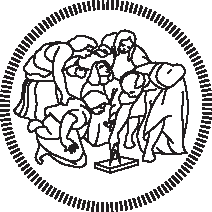
\includegraphics[width=100pt]{assets/logo-polimi-new}\par\vspace{1cm}
    {\scshape\LARGE Politecnico di Milano \par}
    \vspace{1.5cm}
    {\huge\bfseries DD\@: Design Document \par}
    \vspace{2cm}
    {\Large {Alice Piemonti\quad Luca Pirovano\quad Nicolò Sonnino}\par}
    \vfill
    {\large Professor\par
        Matteo \textsc{Rossi}}
    \vfill
    {\large \textbf{Version 1.1} \\ \today \par}
\end{titlepage}
\hypersetup{%
    pdfborder = {0 0 0}
}
\thispagestyle{plain}
\pagenumbering{gobble}
\mbox{}
\newpage
\pagenumbering{roman}
\tableofcontents
\newpage
\pagenumbering{arabic}

\section{Introduction}
\subsection{Purpose}
The purpose of this document is to provide an exhausting explanation about the S2B, focusing in particular on the architecture that will be adopted, the modules of the system and their interfaces.

Furthermore, a runtime view of the core functionalities of the S2B is provided, accompanied by some detailed interactions diagrams that show the message exchanging between the components.

Finally, there are mentions about the implementation, testing and integration processes.

\subsection{Scope}
The application provides different actors that will use the application, which are users, store administrators and store attendants.

\textbf{Users} can access to the application in order to plan their visit to the grocery shop, which can be booked in two different ways. In fact, they can grab the first available ticket (which is called \textit{ASAP} mode) or they can choose a date and time slot in which they plan to visit the store, and also a duration or some articles they are intended to buy, in order to optimize schedules and reduce queues.

\textbf{Store Administrators} can register their shop on the platform, in order to become visible and bookable by users. They can also edit store information (such as opening hours, capacity of slots, etc.) and add or remove the store attendants.

Finally, \textbf{Store Attendants} can sign up with their personal store code in order to monitor entrances through a specific section of the application.

\subsection{Definitions, Acronyms, Abbreviations}
\subsubsection{Definitions}
\begin{itemize}
    \item \textbf{Client-side scripting:} it is performed to generate a code that can run on the client end (browser) without needing the server side processing.
    \item \textbf{Code On Demand:} in distributed computing, it is any technology that sends executable software code from a server computer to a client computer upon request from the client's software.
    \item \textbf{Middleware:} in distributed applications, it represents the software that enables communication and management of data.
    \item \textbf{RESTful:} it s a software architectural style that defines a set of constraints to be used for creating Web services.
    \item \textbf{Slot:} it is a day/time range. It can be reserved by a limit number of users in order to guarantee a maximum number of people who are inside a store in every time of the day.
    \item \textbf{Tier:} it is a row or layer in a series of similarly arranged objects. In computer programming, the parts of a program can be distributed among several tiers, each located in a different computer in a network.
    \item \textbf{Visit:} it refers to the customers entering the shop, and also to their staying time. It is associated to both a certain store and a visit slot.
    \item \textbf{Web Interface:} it permits to use a service only through the web browser.
\end{itemize}

\subsubsection{Acronyms}
\begin{itemize}
    \item \textbf{API:} Application Programming Interface, it indicates on demand procedure which supply a specific task.
    \item \textbf{ASAP:} As Soon As Possible. It refers to the possibility of getting an appointment on the first available slot.
    \item \textbf{DBMS:} DataBase Management System.
    \item \textbf{DD:} Design Document
    \item \textbf{ER:} Entity-Relationship model, it describes interrelated things of interest in a specific domain of knowledge.
    \item \textbf{HTTPS:} Hypertext Transfer Protocol Secure (HTTPS) is an extension of the Hypertext Transfer Protocol (HTTP). It is used for secure communication over a computer network, and is widely adopted on the Internet.
    \item \textbf{MVP:} Minimum Viable Product, it is a version of a product with just enough features to be usable by early customers who can then provide feedback for future product development.
    \item \textbf{RASD:} Requirements Analysis and Specification Document
    \item \textbf{S2B:} Software to Be, it is the one designed in this document and not yet implemented.
    \item \textbf{TLS:} Transport Layer Security, it is a protocol which aims primarily to provide privacy and data integrity between two or more communicating computer applications
\end{itemize}

\subsubsection{Abbreviations}
\begin{itemize}
    \item \textbf{Gn}: goal number n.
    \item \textbf{Rn}: requirement number n.
    \item \textbf{ID}: identifier.
\end{itemize}

\subsection{Revision History}
\begin{itemize}
    \item January 9, 2021: version 1.0 (first release)
    \item \today: version 1.1: \begin{enumerate}
              \item Fixed typos;
              \item Updated Sequence Diagram and related descriptions;
              \item Updated Interface Diagram;
              \item Updated Component Diagram;
              \item Updated ER Diagram;
              \item Detailed description ORM, document's scope, components.
          \end{enumerate}
\end{itemize}

\subsection{Reference Documents}
\begin{itemize}
    \item Requirements Analysis Specification Document (RASD)
    \item UML official specification: \href{https://www.omg.org/spec/UML/}{https://www.omg.org/spec/UML/}
\end{itemize}

\subsection{Document Structure}
\begin{itemize}
    \item \textbf{Section 1: Introduction}\\This section offers a brief description of the document that will be presented, with all the definitions, acryonyms and abbreviations that will be found reading it.
    \item \textbf{Section 2: Architectural Design}\\This section is addressed to the developer team and offers a more detailed description of the architecture of the system. The first part describes the chosen paradigm and the overall split of the system into several layers. Furthermore, an high-level description of the system is provided, together with a presentation of the modules composing its nodes. Finally, there is a concrete description of the tiers forming the S2B.
    \item \textbf{Section 3: User Interface Design}\\This section is useful for graphical designers of the S2B and contains several mockups of the application, together with some charts useful to understand the correct flow of execution of it. The presented mockups refers to the client-side experience.
    \item \textbf{Section 4: Requirements Traceability}\\This section acts as a bridge between the RASD and DD document, providing a complete mapping of the requirements and goals described in the RASD to the logical modules presented in this document.
    \item \textbf{Section 5: Implementation, Integration and Test Plan}\\The last section is again addressed to the developer team and describes the procedures followed for implementing, testing and integrating the components of our S2B. There will be a detailed description of the core functionalities of it, together with a complete report about how to implement and test them.
\end{itemize}

\newpage

\section{Architectural Design}
\subsection{Overview}
\begin{figure}[H]
    \begin{center}
        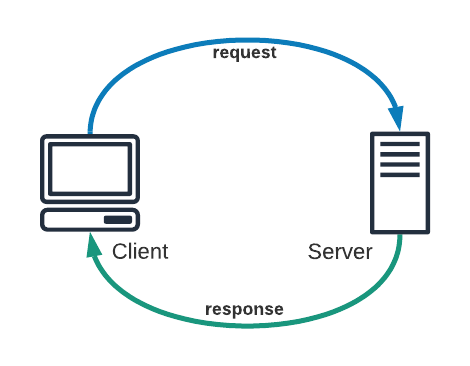
\includegraphics[width=\textwidth/2]{assets/Architectural-Design/Client-Server.png}
        \caption{Client-Server paradigm}\label{client_server_par}
    \end{center}
\end{figure}

As figure \ref{client_server_par} represents, the system is a distributed application which follows the common known client-server paradigm.

In particular, there are two different types of client, which makes it either thin and fat at the same time.

The first one is a RIA \textit{Web Application}, which is by definition a thin client, because of its total dependency from the server.
This type of client does not contain the application business logic, but only the presentation layer.

The second one, instead, is a mobile application, which contains an internal database in order to make it less dependent from the server. This aspect makes it a more thick client.

In both cases the server is \textit{fat} and contains all the data management and business logic.

In this section the architecture will be described in an easy way, justifying all the choices for adopted patterns.

\begin{figure}[H]
    \begin{center}
        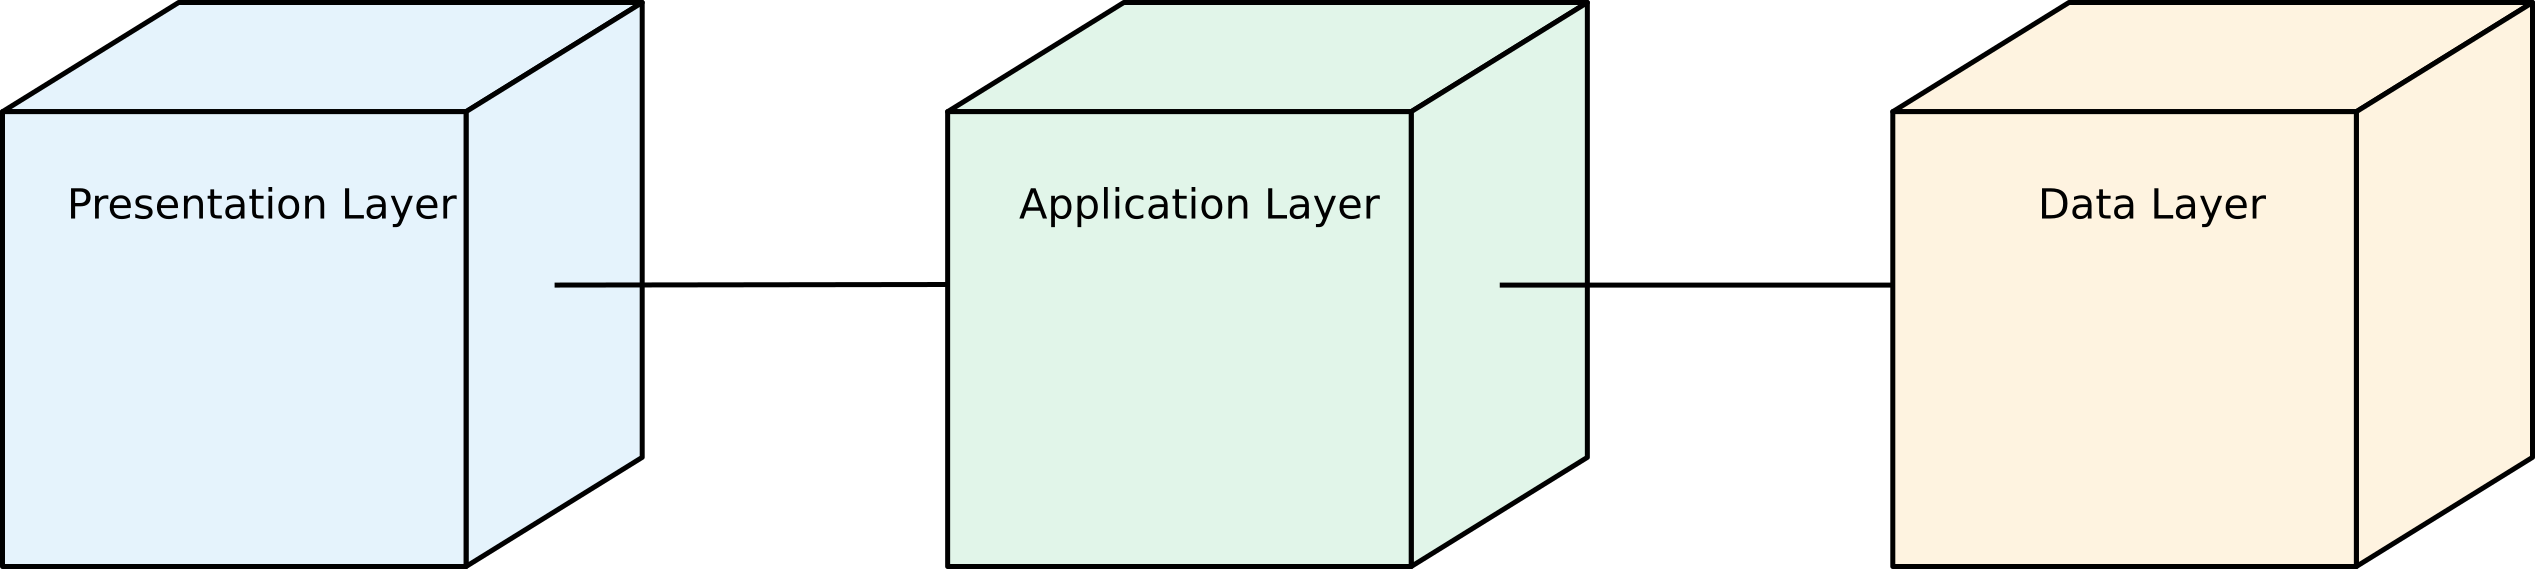
\includegraphics[width=\textwidth]{assets/Architectural-Design/3-tier.png}
        \caption{Three layers application}\label{three_tier_desc}
    \end{center}
\end{figure}

In figure\ref{three_tier_desc} the three S2B layers are shown, which respectively are:
\begin{itemize}
    \item \textbf{Presentation Layer:} it manages the presentation logic and, consequently, all the interactions with the end user. This is also called \textit{rendering layer}.
    \item \textbf{Application (Logic) Layer:} it manages the business functions that the S2B must provide.
    \item \textbf{Data Layer:} it manages the safe storage and the relative access to data.
\end{itemize}

As shown in the high level representation of figure \ref{three_tier_application} the S2B is divided into three layers that are physically separated by installing them on different tiers. A tier is a physical (or a set of) machine, each of them with its own computational power.

The application described in this document is composed by four tiers.

\begin{figure}[H]
    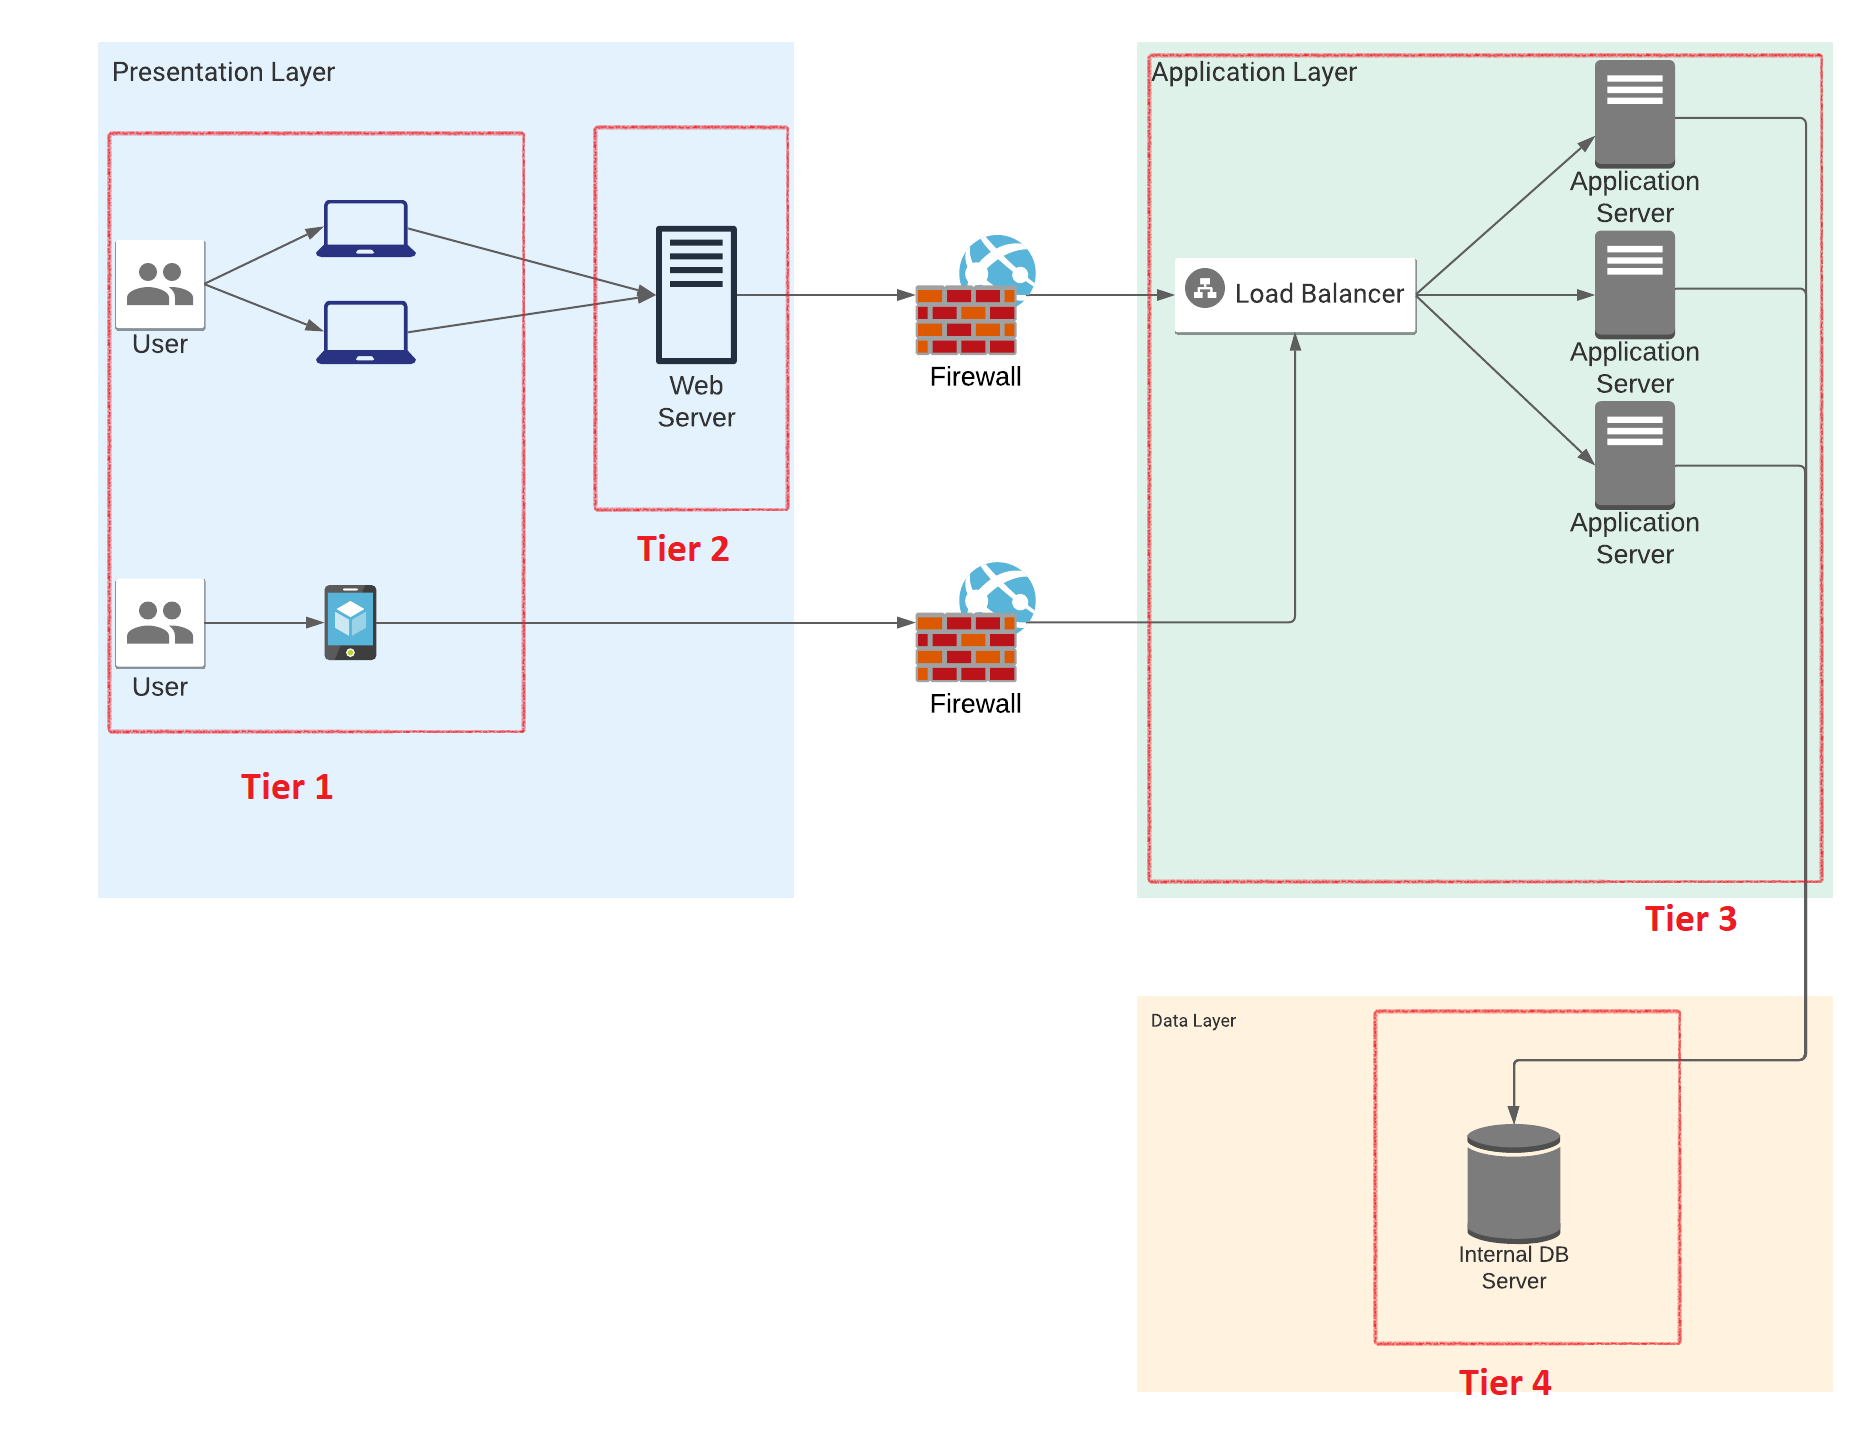
\includegraphics[width=\textwidth]{assets/Architectural-Design/ApplicationArchitecture.png}
    \caption{Architecture of the application}\label{three_tier_application}
\end{figure}

The service is supposed to be accessed through both a web interface and a mobile application, and this is valid for all kinds of users.

To make possible the construction of the web application, a client-side scripting paradigm will be adopted; this one will be described in detail in the final section of this document.

The architectural figure divides the application in the layers described above, and contains some replicated Web Servers, which act as a middleware between the user's browser and the application servers.
In case of using the mobile application, instead, the core of the software installed on user's device will interfaces with the business layer's APIs, which send and receive all the information in order to work properly directly to the application servers.

Finally, the application servers interfaces with the DBMS APIs, in order to retrieve and store the data required for the considered computation.

The applications servers are expected to be stateless, according to the REST standard definitions (more details in section \ref{REST}).
For accessing the data, they will use an ORM programming technique in order to interface with the DBMS exploiting the advantages of the object-oriented paradigm.

The nodes are separated by firewalls to guarantee a higher level of security of the whole system.

All the component will be described in depth in the following sections.

In case of third module development, which permits a custom deploy on buyer organization's servers, the entire architecture will be deployed and then configure on that servers, without interfacing with CLup ones.

\subsection{Component View}

\begin{figure}[H]
    \begin{center}
        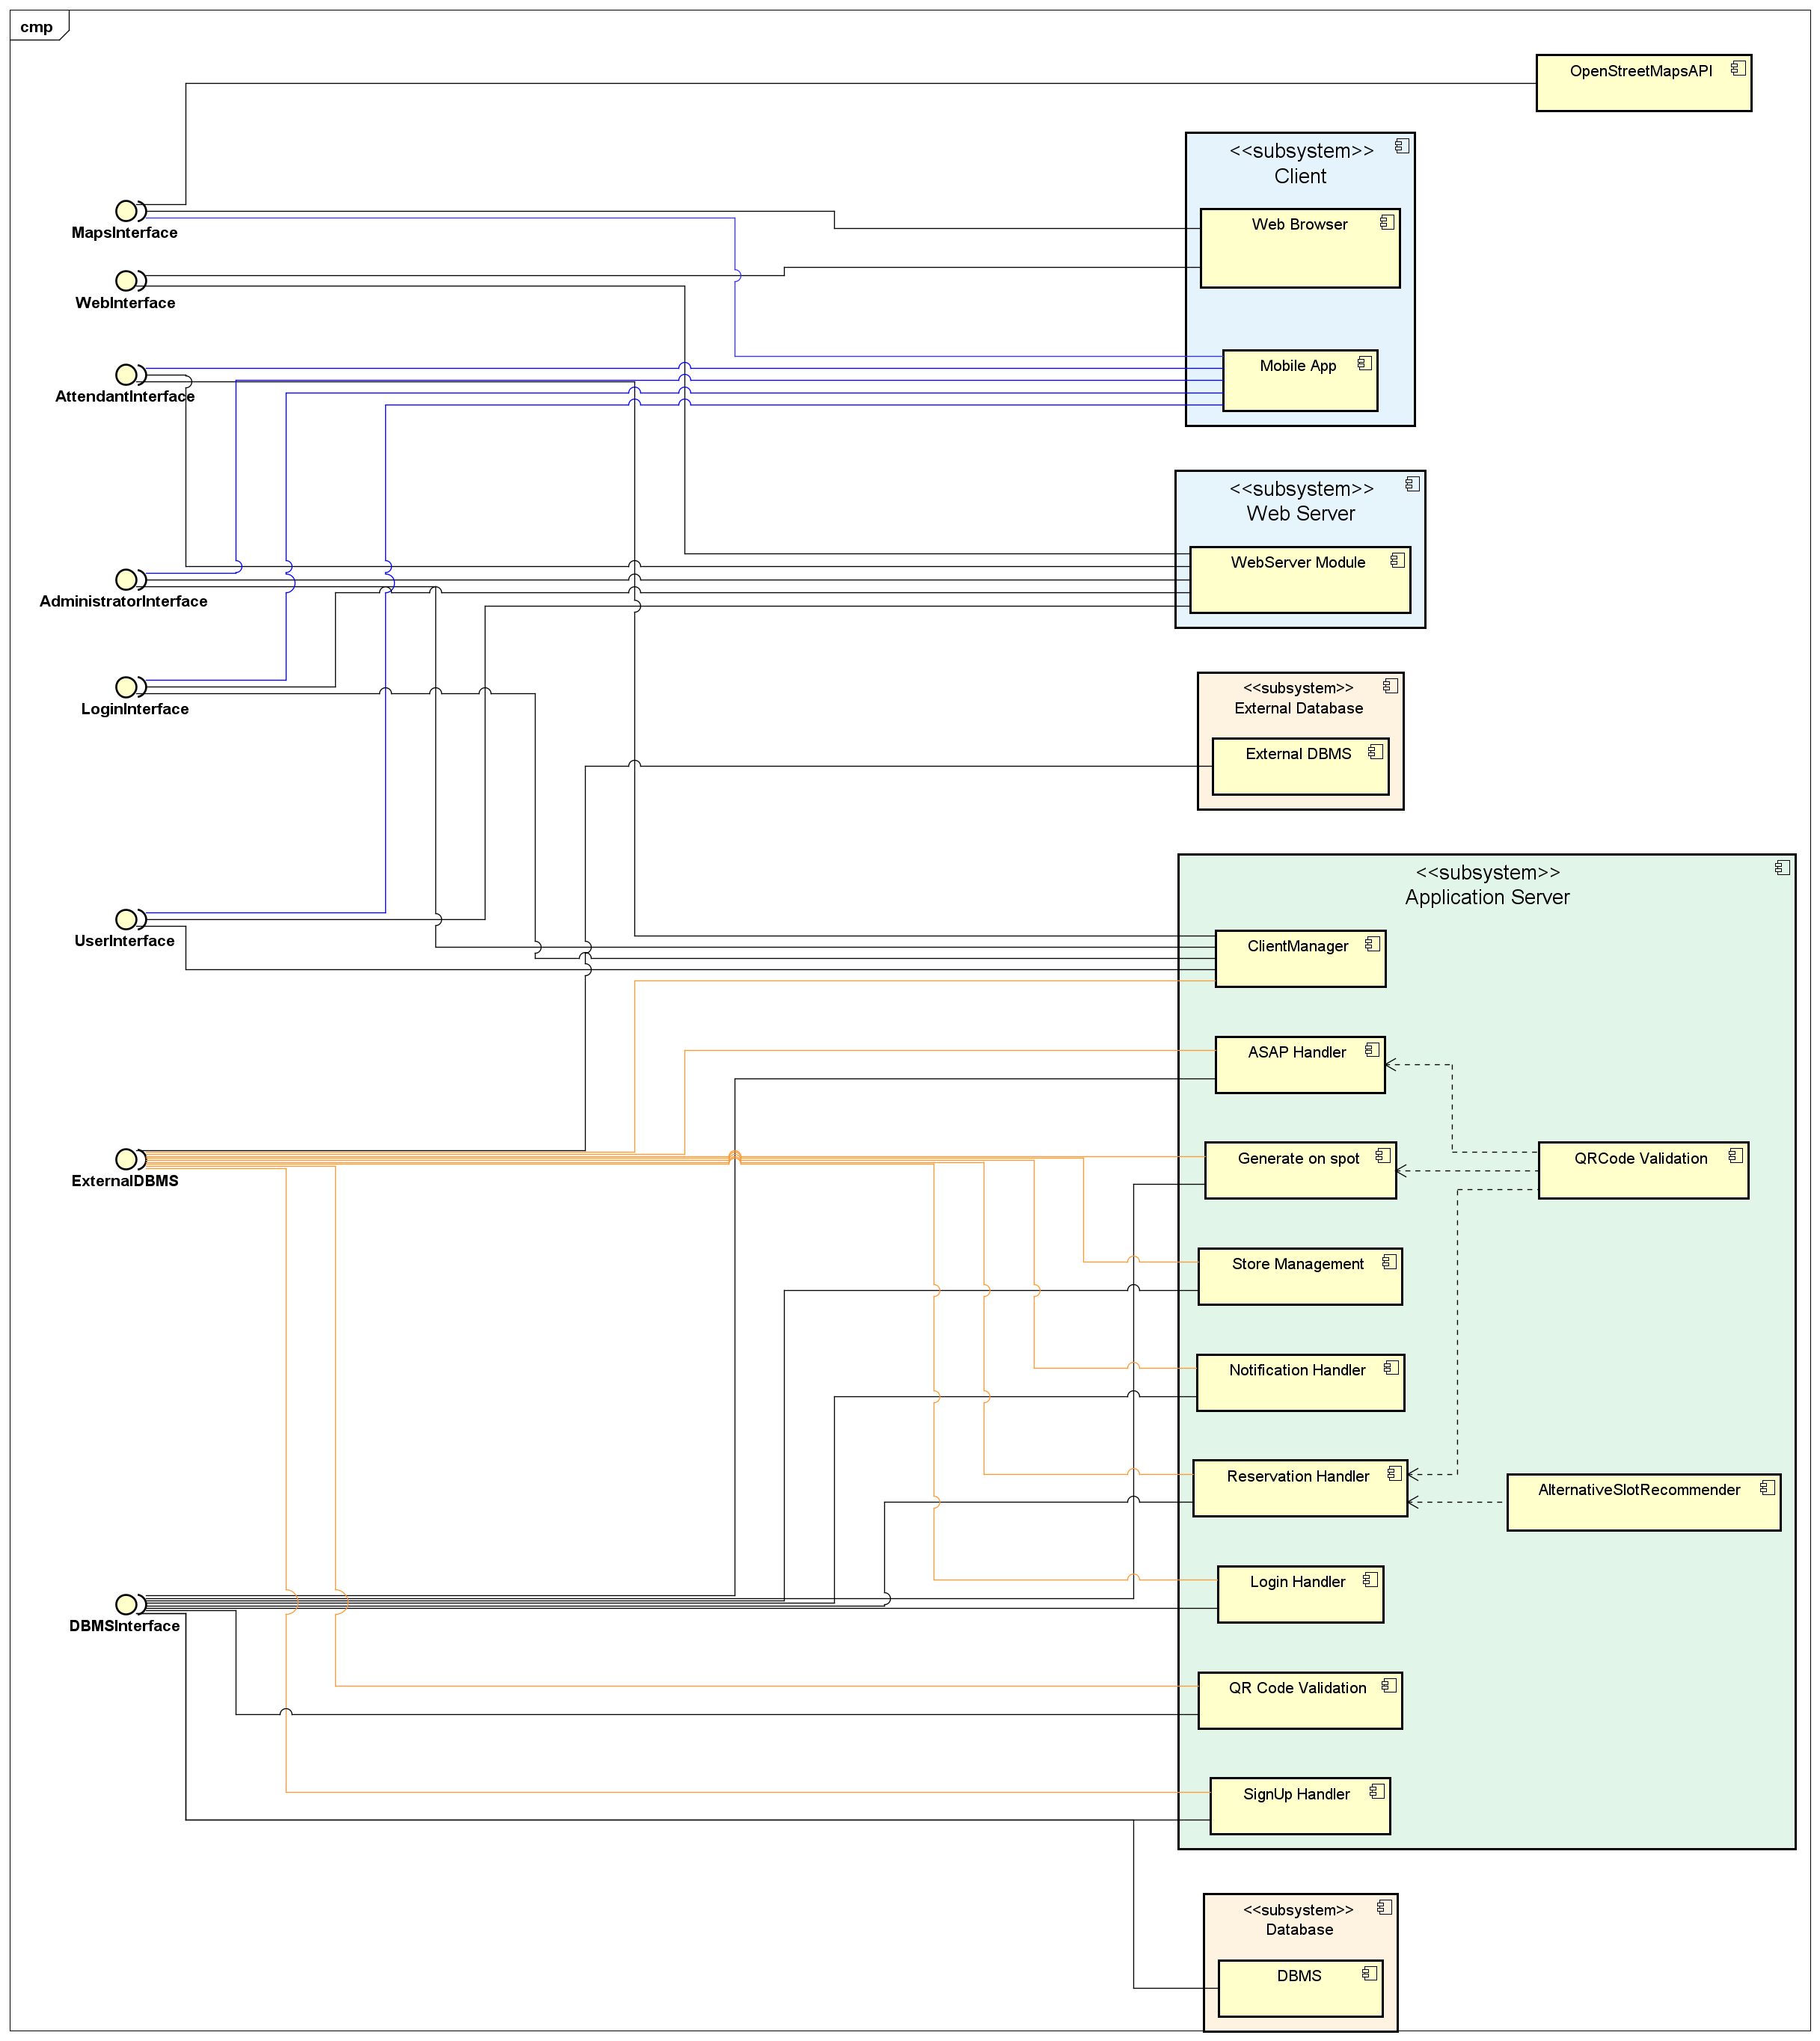
\includegraphics[width=\textwidth]{assets/Architectural-Design/ComponentDiagram.png}
        \caption{Component Diagram}\label{component_diagram}
    \end{center}
\end{figure}

In figure \ref{component_diagram} we can see a more detailed diagram representing the layers described before.

The web server has the function to route the browser requests to the application server and send back its responses.

\begin{itemize}
    \item \textbf{Client Manager}\\This module handles all the requests made by the client. At the beginning, when the client is not logged in, the module offers a \textit{loginInterface} which permits to execute a sign up or sign in operation. Once the client has logged in, the module shows only the other types of interfaces relying on the type of log in: a client logged as a user will exploit the \textit{UserInterface}, a store attendant an \textit{AttendantInterface} and a store administrator an \textit{Administrator Interface}.
    \item \textbf{Login Handler}\\This component handles the process of sign in. It receives the credentials inserted by the user (which are username and password) and checks for a correspondence in the database. If it found something, the user becomes authenticated and can continue to the correct private area.
    \item \textbf{SignUp Handler}\\This module's goal is to permit a user registration to the CLup service. There are three different sign up processes, one for each account type. The default registration flow firstly allows to register as a general user, since the application is intended to be used mostly by customers. However, at the beginning of the process, a prompt permits to switch the type of sign up from \textit{User} to \textit{Attendant} or \textit{Administrator}. Some data will be asked to the registering client, such as an email and a password.
    \item \textbf{ASAP Handler}\\This component handles the process of the MVP (see RASD section 1.1), which is the \textit{Retrieve a ticket} functionality. A registered and authenticated user selects the desired grocery store and requests, through a button, a new ticket. The S2B then provides an unique queue number, an estimated waiting time and a QRCode which will be user to check-in at the entrances of the store.
    \item \textbf{Reservation Handler}\\This is the second module of our S2B described in s. 1.1 of RASD document. Through this component, the registered and authenticated user can select a store and book a visit slot in the desired date and time (if available). The component can optionally receive from user an estimated duration of the visit and a shopping list, in order to optimize people flows in the structure. Once the computation has finished, the component returns to user a confirmation, together with a QRCode to check-in.
    \item \textbf{Notification Handler}\\The goal of this component is to handle notifications of imminent calling of a ticket. In fact, when a number is going to be called, a trigger is generated, which sends an instant notification to the user who retrieved that ticket.
    \item \textbf{Generate on spot}\\This module handles the manual procedure of generating a ticket on the spot. In fact, when a customer cannot sign up to CLup service, there is the possibility of going physically to the desired store and ask to an attendant to be queued up. The attendant, through this component, sends a request of retrieving a ticket, and the server returns the first slot available. This ticket is then printed, together with a QRCode generated from the system.
    \item \textbf{QRCode Validation}\\The goal carried out by this component is the \textit{entrances monitoring} one. When a user arrives at the store, the attendant scans the QRCode generated from the application (or printed) and lets the user entering the structure. The attendant scans the ticket (through CLup mobile app) with the integrated camera of a smartphone. The application then sends a request of check-in to the server, which responds with a status of the request (which can be either valid or invalid).
    \item \textbf{QRCode Generation}\\The goal of this module is to generate the QR Code of the ticket from a pre-defined string, which is the unique id of the ticket.
    \item \textbf{Alternative Slot Recommender}\\This component's aim is to suggest alternative slots to the end user, relying on people flows estimation which derives from an analysis of all bookings' time slot and duration time.
    \item \textbf{Store Management}\\This last module handles the store administrator's personal area. In fact, it permits editing store information, which includes opening hours, maximum slots capacity, booking management and so on.
\end{itemize}

\subsection{Deployment View}

\begin{figure}[H]
    \begin{center}
        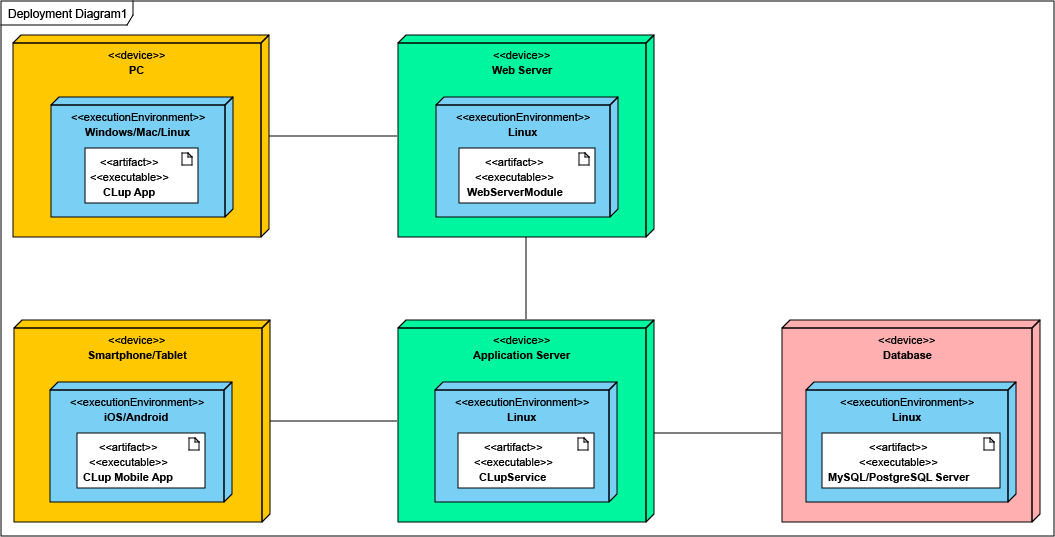
\includegraphics[width=\textwidth]{assets/Deployment-Diagram/DeploymentDiagram1.png}
        \caption{Deployment Diagram}\label{deployment_diagram}
    \end{center}
\end{figure}

The deployment diagram in figure\ref{deployment_diagram} shows the needed components for a correct system behavior, except the Maps APIs and the Authentication APIs ones.

Each device has its own Operating System where the software runs. The tiers in the image are the following:
\begin{itemize}
    \item \textbf{Tier 1:} it is the client machine, which can be a computer with a web browser (running, for example, on Windows 10 OS) or the downloadable mobile application (available on both Apple's store and Google's Store).
    \item \textbf{Tier 2:} it includes the replicated web servers, which do not execute any business logic, but simply receive requests from the client, route them to the application servers and serve an HTML file fo the client, which will build the page thanks to client-side scripting. They also append the styling logic of the page (CSS sheets, JS sheets, etc.).
    \item \textbf{Tier 3:} it contains the application servers, which run the core functionalities of the S2B. The whole application layer is mapped into this tier, which communicates to the client tier through APIs, which will be used from the web servers (in case of webapp) and the native application (in case of mobile app download). Furthermore, it communicates to the data tier through the DBMS gateway.
    \item \textbf{Tier 4:} it is composed by the DBMS servers. They store the data and execute actions on it, according to the instruction given by the application servers.
\end{itemize}

\subsection{Runtime View}
All the following diagrams represent the runtime view from the mobile app's perspective, in order to increase readability, the web app's perspective isn't shown as it only differs from the other one by using the web server's module before calling the Application Server.\\
Every interface use REST API through HTTP GET or/and POST calls using urls, where the " \textbf{..} " before every path it's to be intended as the IP address + port of the server or the domain.\\
The login and registration on the mobile app is only permitted for store attendants or customers, managers need to use the web app interface.
\subsubsection{Sign Up}
\begin{figure}[H]
    \begin{center}
        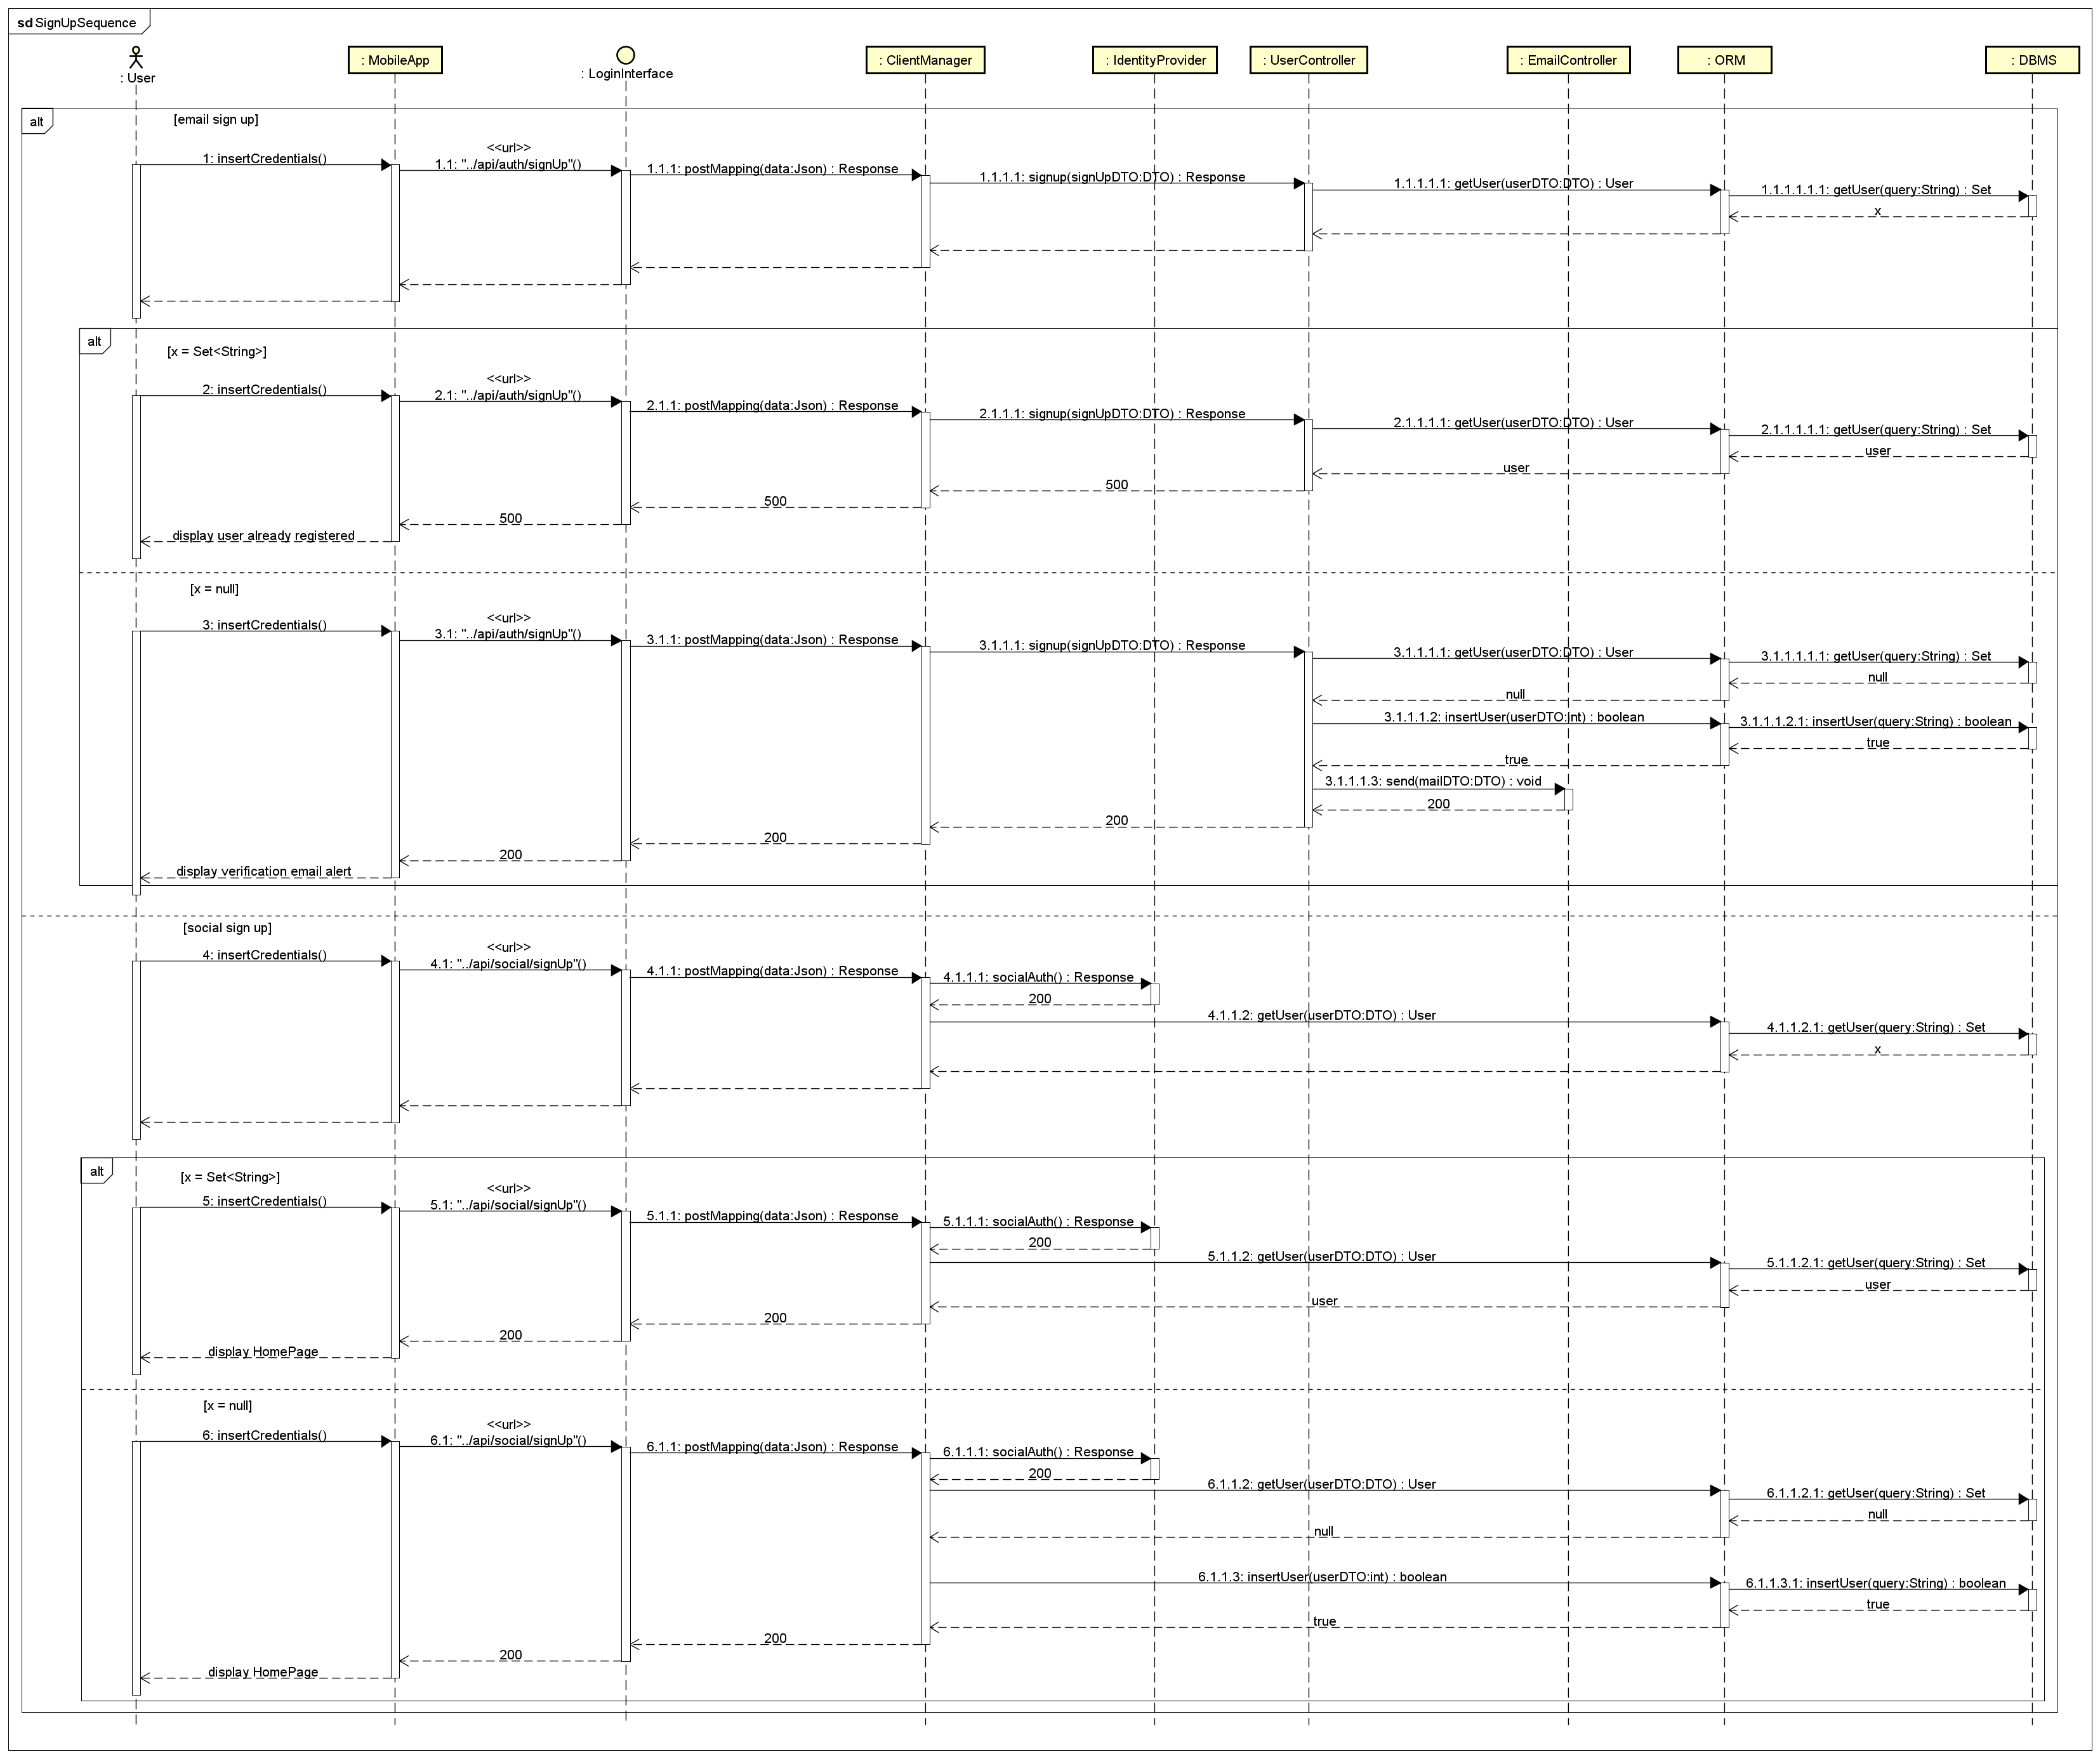
\includegraphics[width=\textwidth]{assets/Sequence-Diagram/SignUpSequence.png}
    \end{center}
\end{figure}
The diagram above represents the process of signing up a user (store attendant and administrator  registration are omitted in order to avoid unnecessary repetitions).\\
There two possible situations:
\begin{itemize}
    \item User is already registered;
    \item User isn't already registered.
\end{itemize}
The two situations differ only after submitting the user's data to the database and are analyzed below.\\
The user is presented with two choices: registering via social network or with an email and password; if the user chooses the first one, they click on their preferred social network displayed in the Mobile App.\\
Afterwards the app sends the request to the ClientManager through the LoginInterface (url "../api/social/signUp"), accessing later the IdentityProvider.\\
The IdentityProvider returns user's info to the ClientManager which generates a userDTO, passing to the ORM and ultimately to the DMBS.\\
Based on the returned value of the DBMS the ClientManager inserts the User into the database or returns 200 response's status code (as shown above).\\
If the user decides the login via email, the path from the Mobile App to the ClientManager remains unchanged but this last one component delegates the database's query to the UserController (via ORM and DBMS).\\
If the returned value isn't null the UserController sends a 500 response's status code, warning the User that a previous registration exists.\\
If, instead, the DBMS returned null then the Uses is inserted to the database and lately the UserController via an EmailController sends an email to the provided one and displays to the user the instructions for the verification.\\
\subsubsection{Login}
\begin{figure}[H]
    \begin{center}
        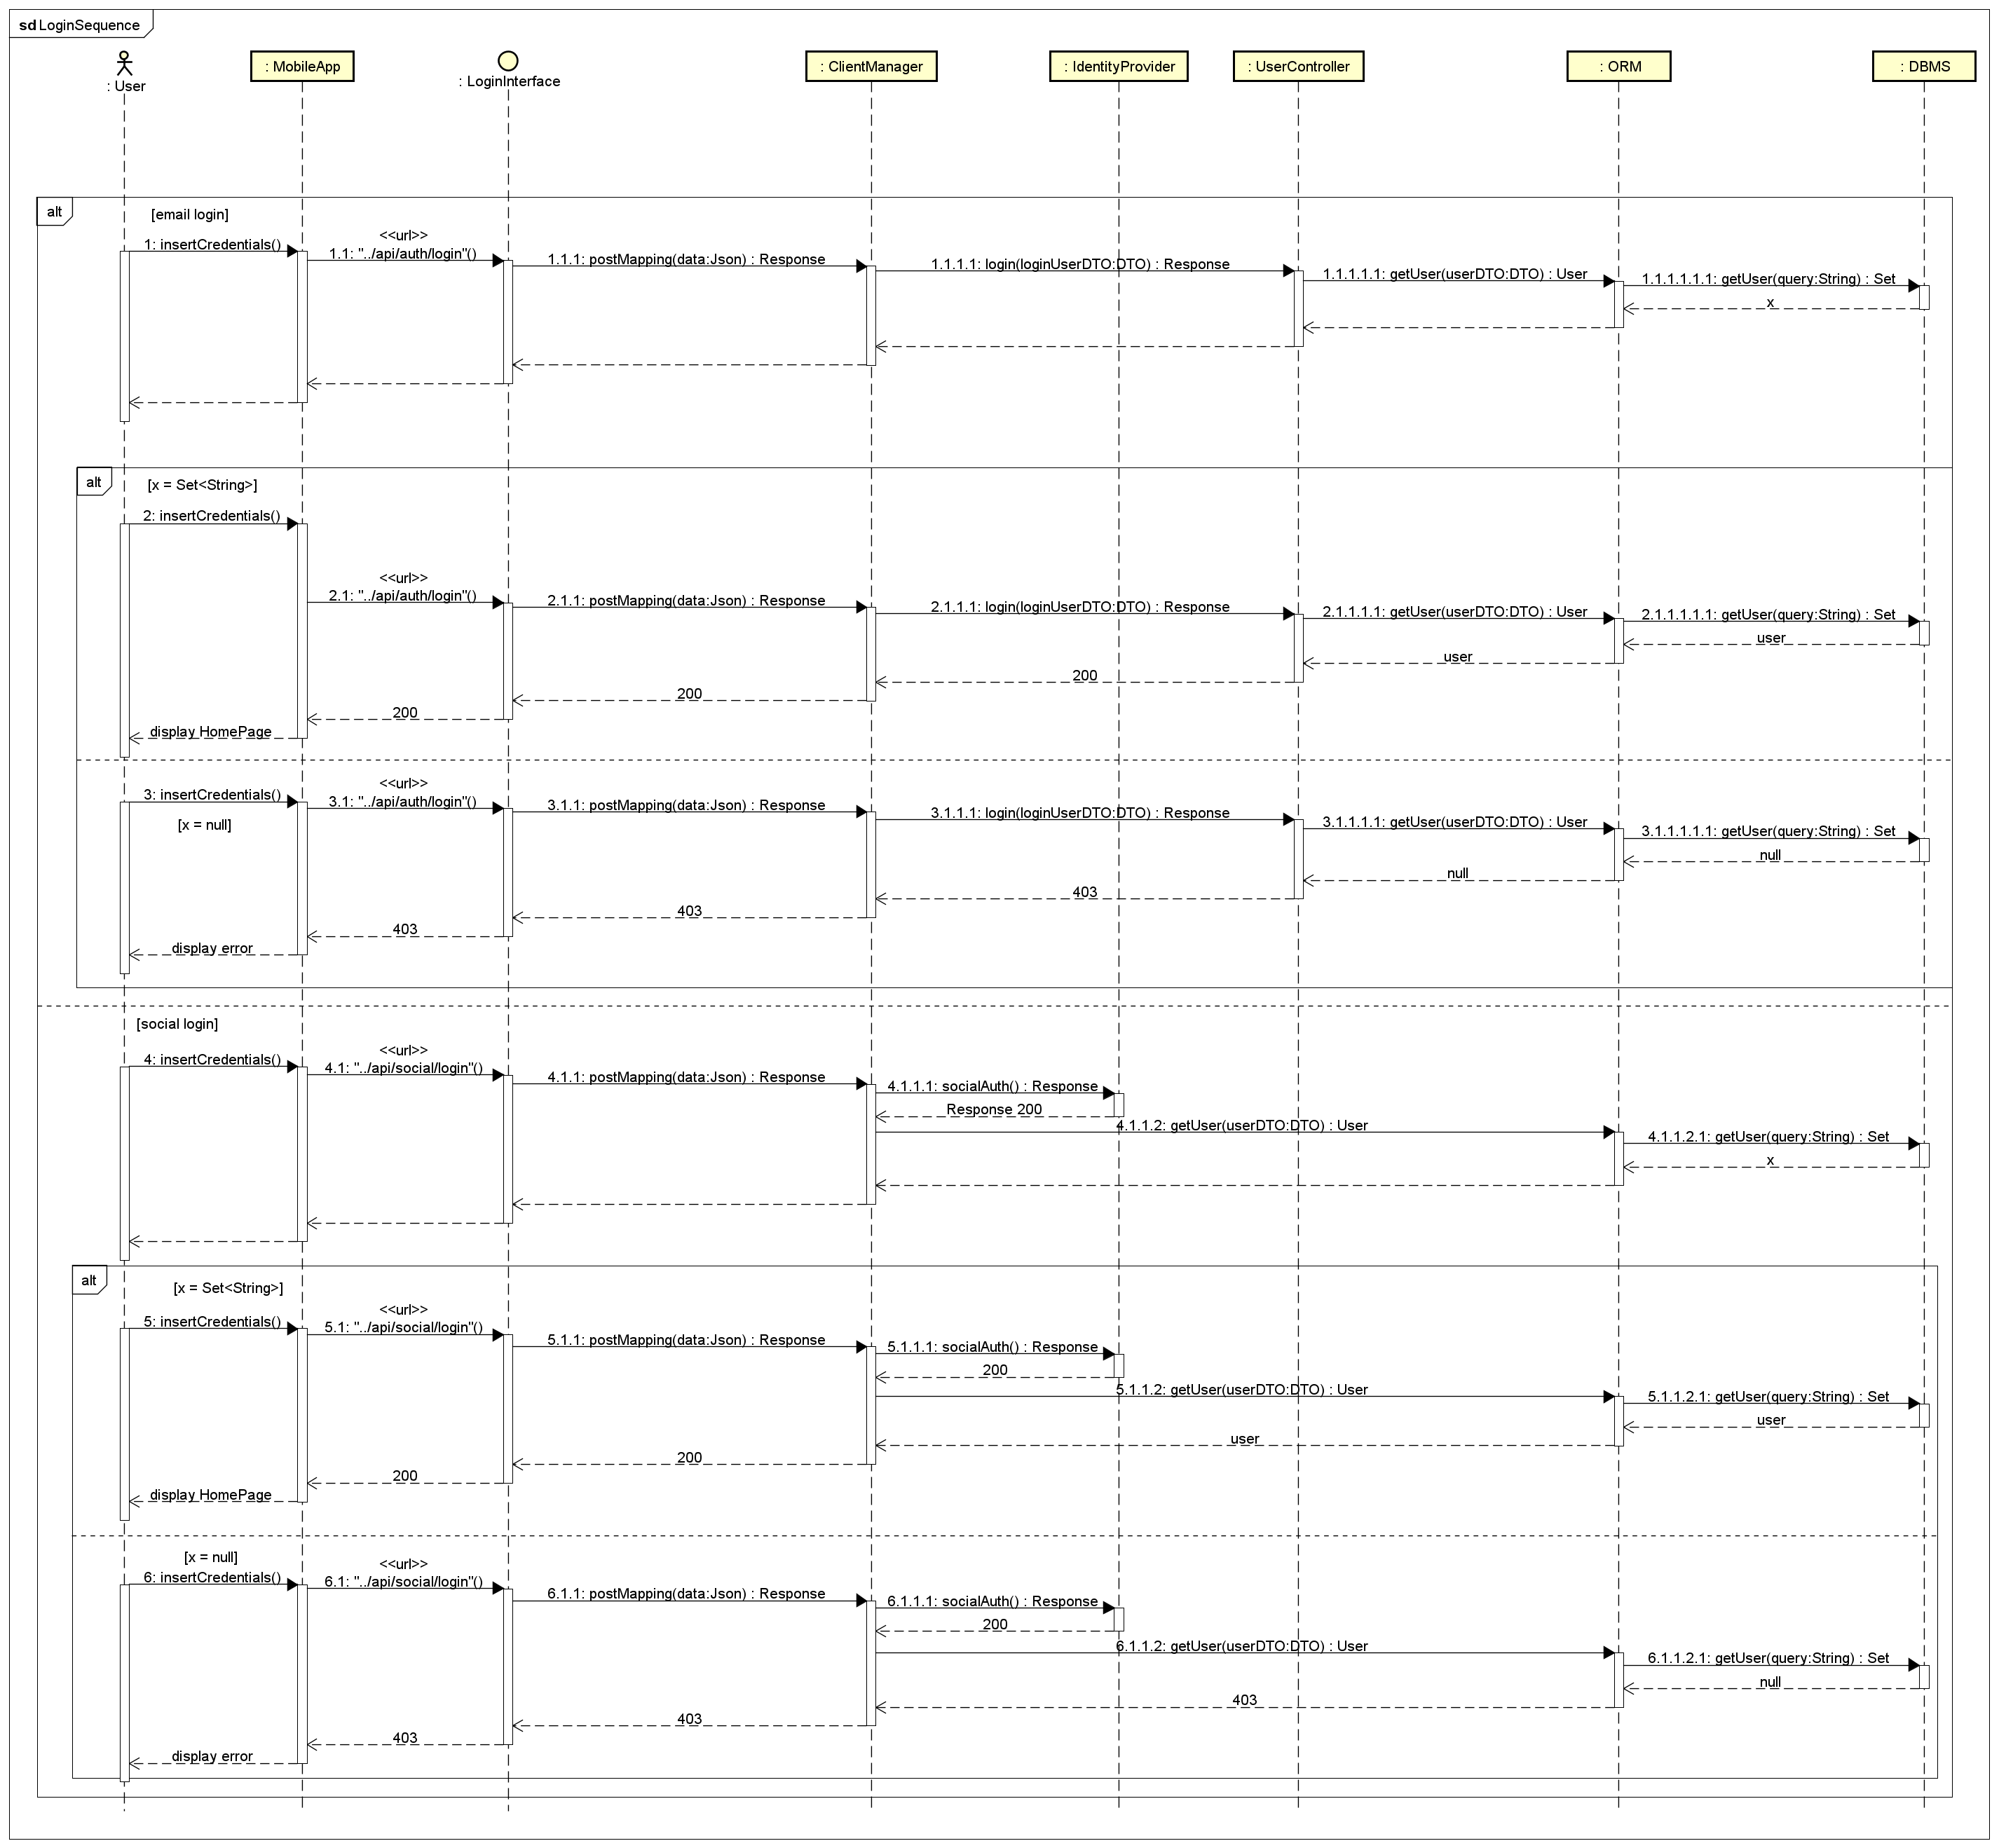
\includegraphics[width=\textwidth]{assets/Sequence-Diagram/LoginSequence.png}
    \end{center}
\end{figure}
The user chooses their preferred login method, whether it's social network or email and password.\\
If the first one is chosen, then the MobileApp sends the request, through the LoginInterface ("../api/social/login") to the ClientManager.\\
After requesting user credentials to the IdentityProvider, the ClientManager interrogates the DBMS (via ORM) and searches for the credentials retrieved.\\
If the returned value is null
After the user inserted their social account credentials or CLup's credentials, they are checked by the LoginHandler through a query; if this one returns no values then a status error message is sent to the App, stating that the user isn't registered.\\
Otherwise the user is redirected to their home page.
\subsubsection{Retrieve a ticket}
\begin{figure}[H]
    \begin{center}
        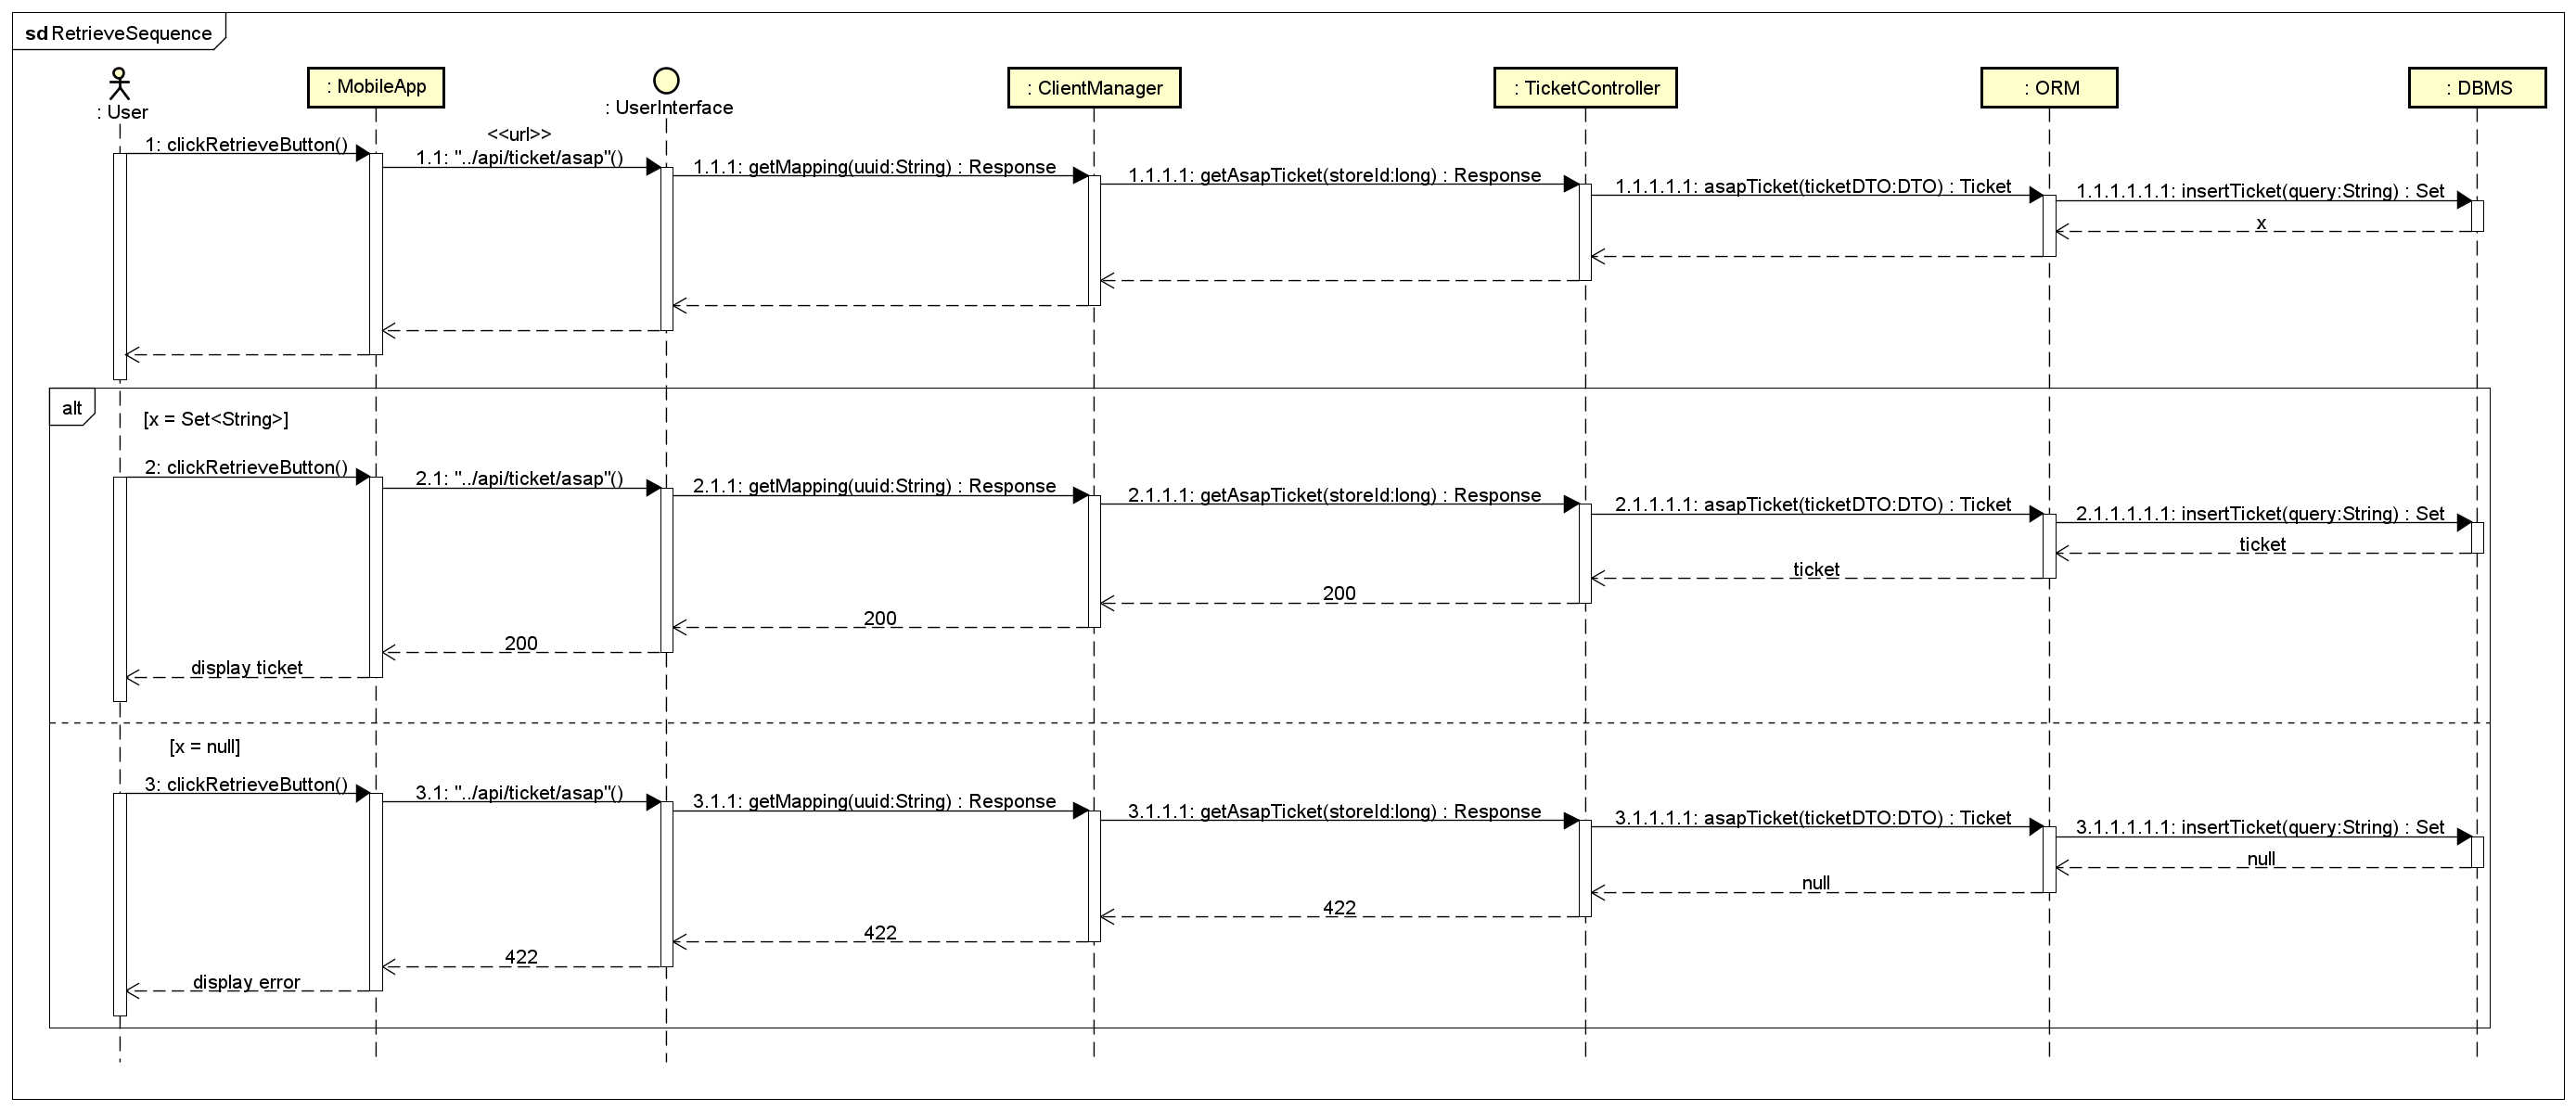
\includegraphics[width=\textwidth]{assets/Sequence-Diagram/RetrieveSequence.png}
    \end{center}
\end{figure}
The process of retrieving a ticket is used by any User in order to generate and queue a ticket for the current day. \\
The User navigates to their home page and presses the button assigned to this function.\\
Afterwards the App sends the request to the ClientManager, which routes it to the RetrieveHandler. \\
The component checks the database to see if there is an available slot.\\
If the query is successful, the RetrieveHandler generates a unique QR code by transferring the data to the QRCodeGenerator; right after this step, the RetrieveHandler sends the ticket info to the ClientManager and finally to the app.\\
If the query returns no values, then the RetrieveHandler warns the ClientManager which sends an error message to the App.

\subsubsection{Make a reservation}
\begin{figure}[H]
    \begin{center}
        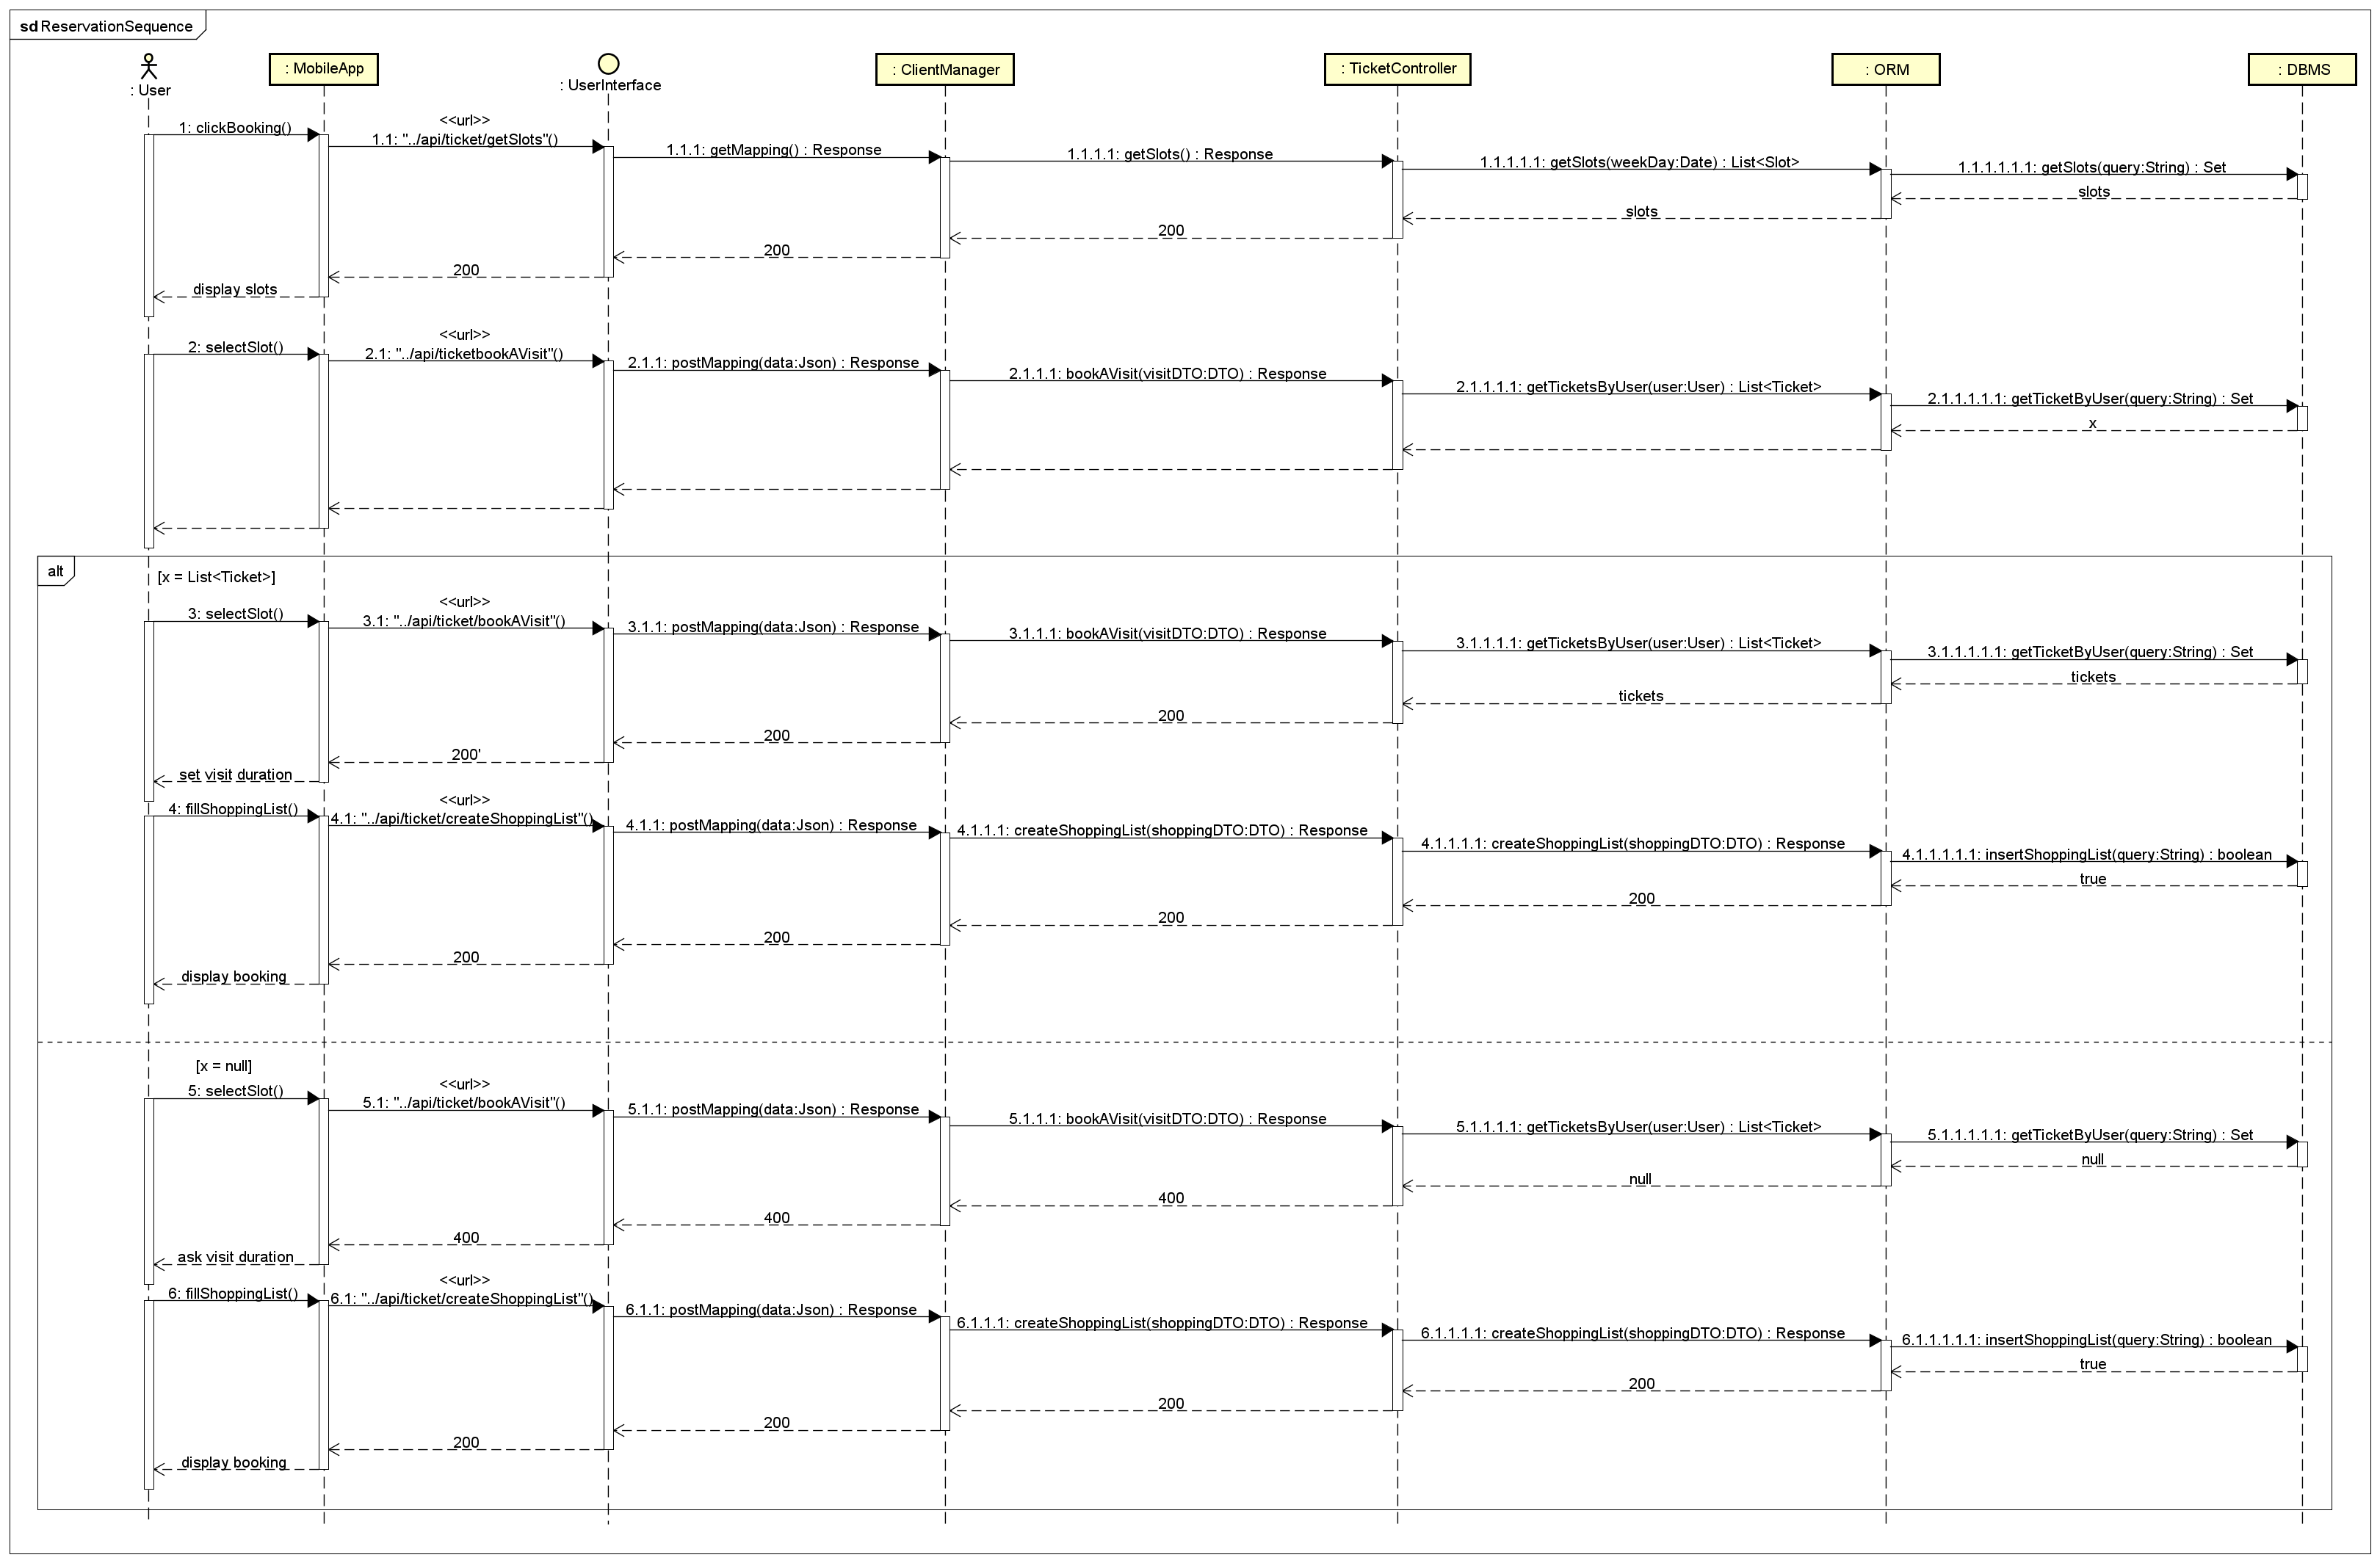
\includegraphics[width=\textwidth]{assets/Sequence-Diagram/ReservationSequence.png}
    \end{center}
\end{figure}
Booking a visit is a process which involves the ClientManager, the ReservationHandler and the QRCodeGenerator.\\
It starts with the User pressing the dedicated button and requesting a reservation, then the App forwards their request to the ClientManager which sends it to the ReservationHandler.\\
This handler checks the database for all available slots and, after receiving the results, generates alternatives for the most popular slots based on a different schedule or store.\\
The User chooses their preferred slot by pressing it, this action triggers the request from the App to ClientManager and to the ReservationHandler, which checks again if the slot is valid (otherwise it returns an error leading to the start of the reservation process) and claims it in the database.\\
Afterwards the ReservationHandler checks the database for previous bookings; if the search is successful, the handler proceeds to generate a visit duration based on the collected data, otherwise the visit's duration request is transferred to the ClientManager and App so the user can specify it.\\
Then it generates the ticket with the help of the QRCodeGenerator and requests the filling of the shopping list, then sends it to the Database.\\
Both of the previous actions are optional and at the User's discretion.
\subsubsection{Remove a reservation}
\begin{figure}[H]
    \begin{center}
        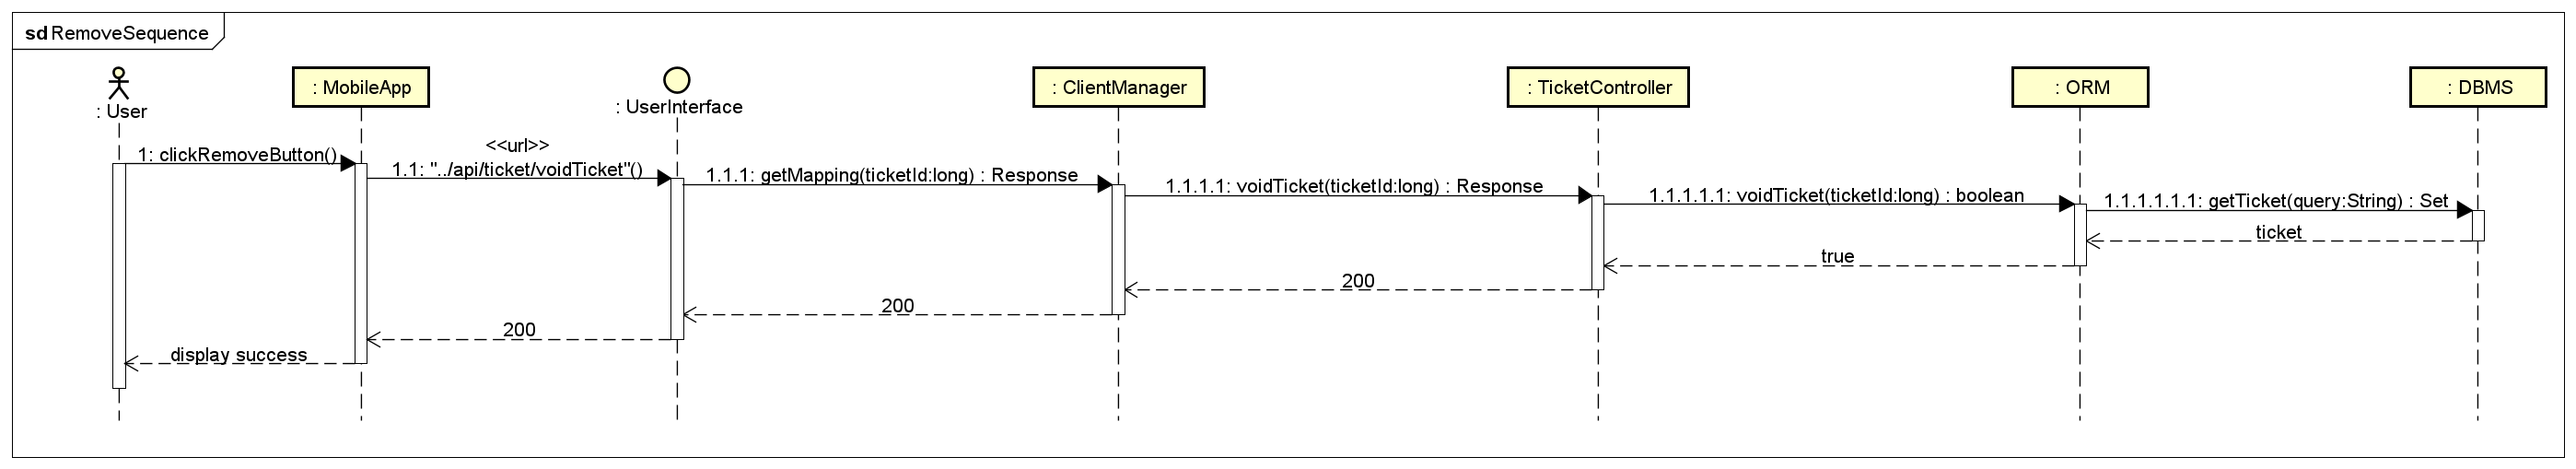
\includegraphics[width=\textwidth]{assets/Sequence-Diagram/RemoveSequence.png}
    \end{center}
\end{figure}
The above diagram describes the process of removing a reservation.\\
The user accesses the specific page and selects the slot to be removed, this sends the request to the ClientManager and to the ReservationHandler.\\
The handler updates the database by removing the selected slots from the user's data and returns the confirmation. \\
\subsubsection{Release a ticket}
\begin{figure}[H]
    \begin{center}
        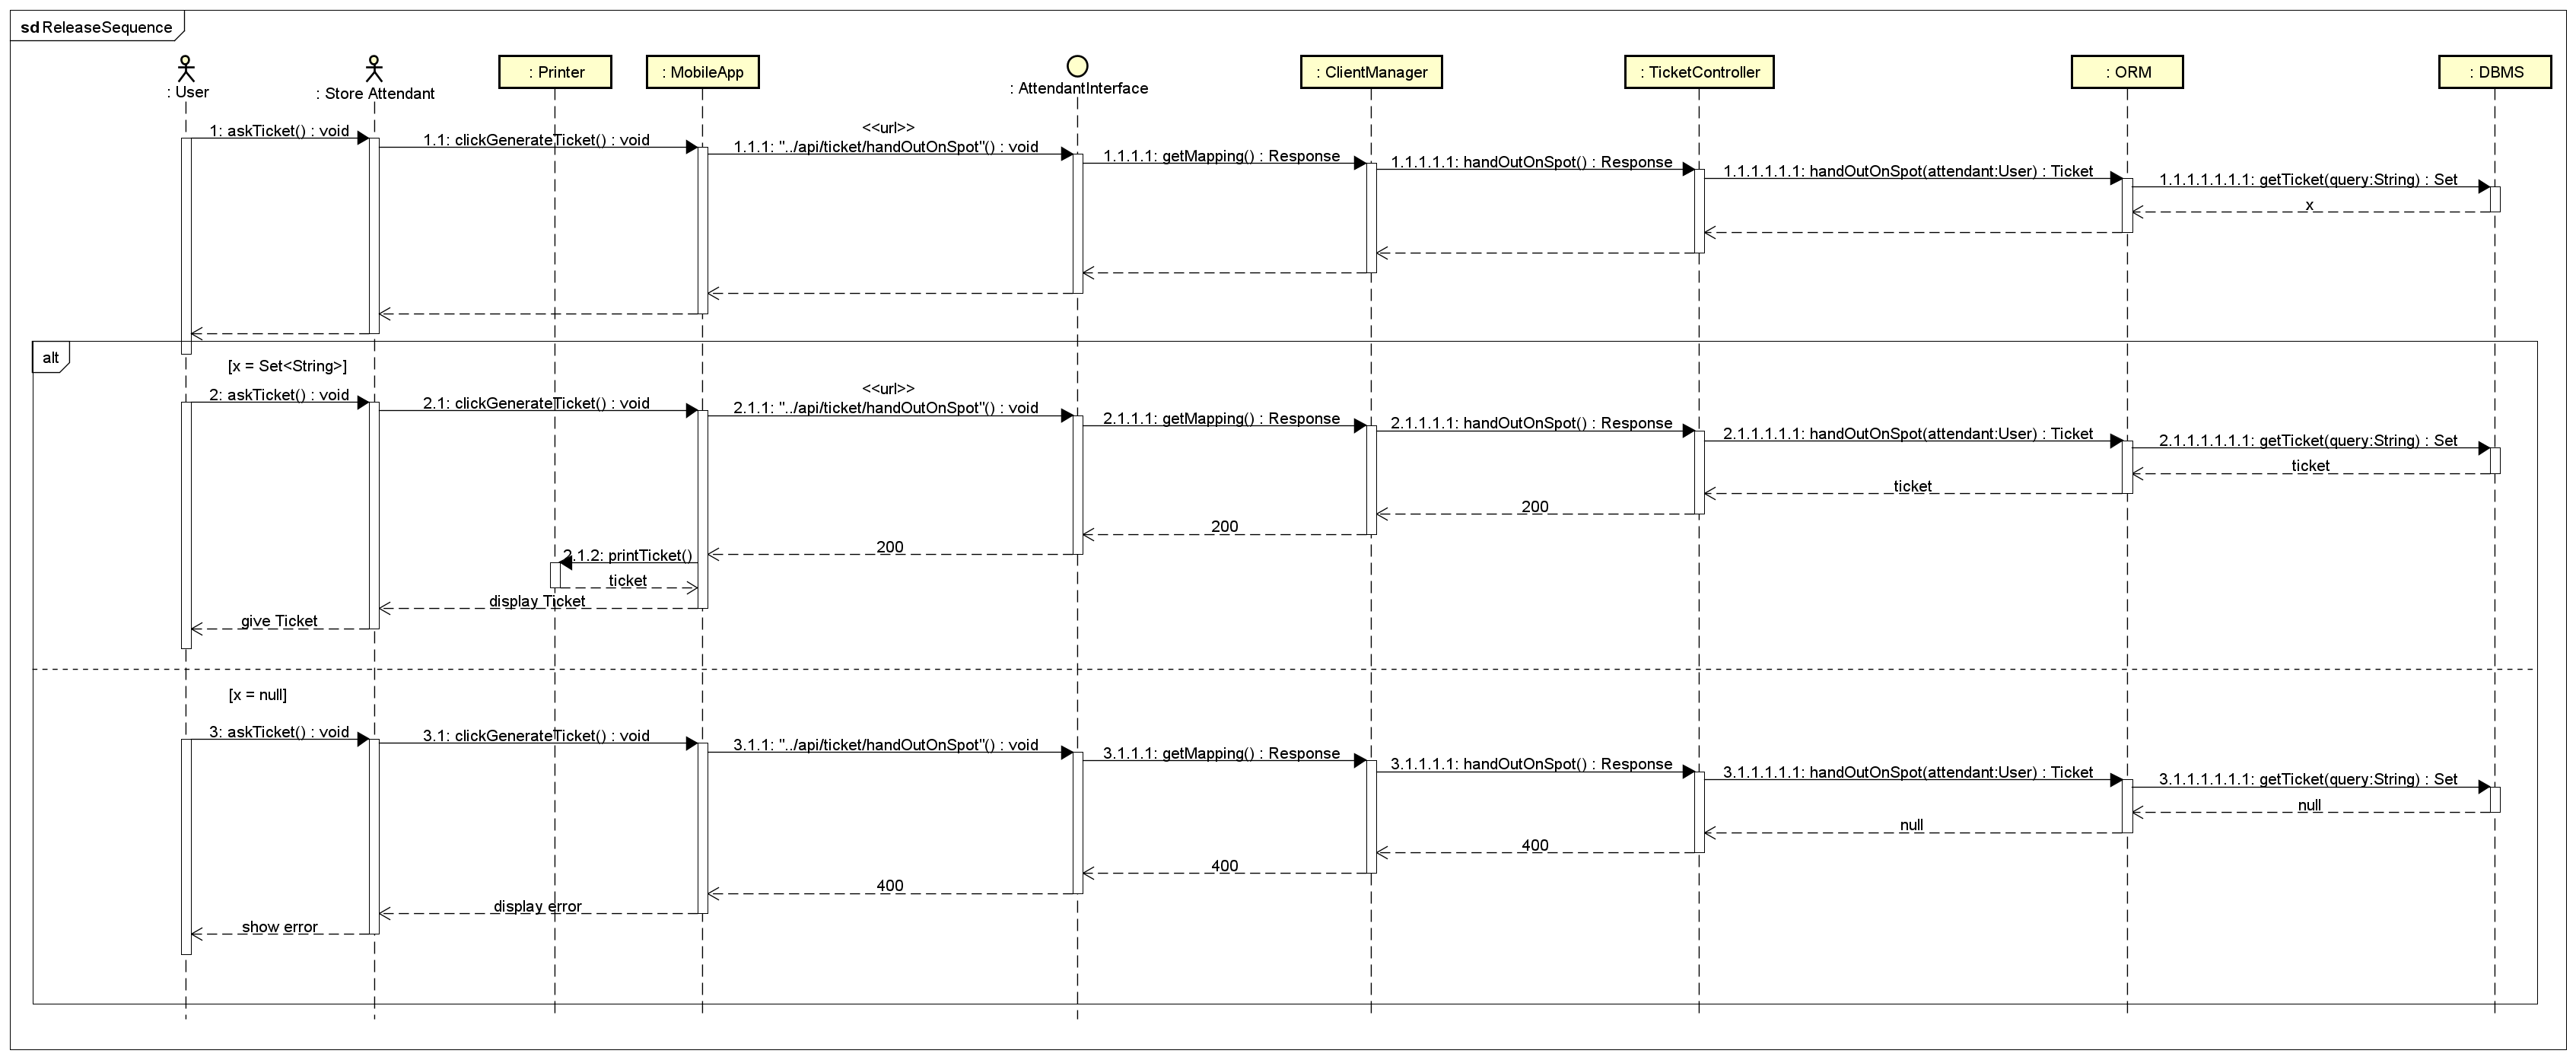
\includegraphics[width=\textwidth]{assets/Sequence-Diagram/ReleaseSequence.png}
    \end{center}
\end{figure}
If a customer can't install the app, they can still ask the staff to generate a ticket directly on the spot as shown above.\\
The Store Attendant navigates to the right page and requests a new ticket from the App to the ClientManager, which forwards it to the GenerateOnSpot handler.\\
The handler checks the database for the closest free slot of the current day: if successful it generates a ticket with its own QR code (using the QRCodeGenerator component) and sends it to the App; it sends an error otherwise.\\
\subsubsection{Scan QR code}
\begin{figure}[H]
    \begin{center}
        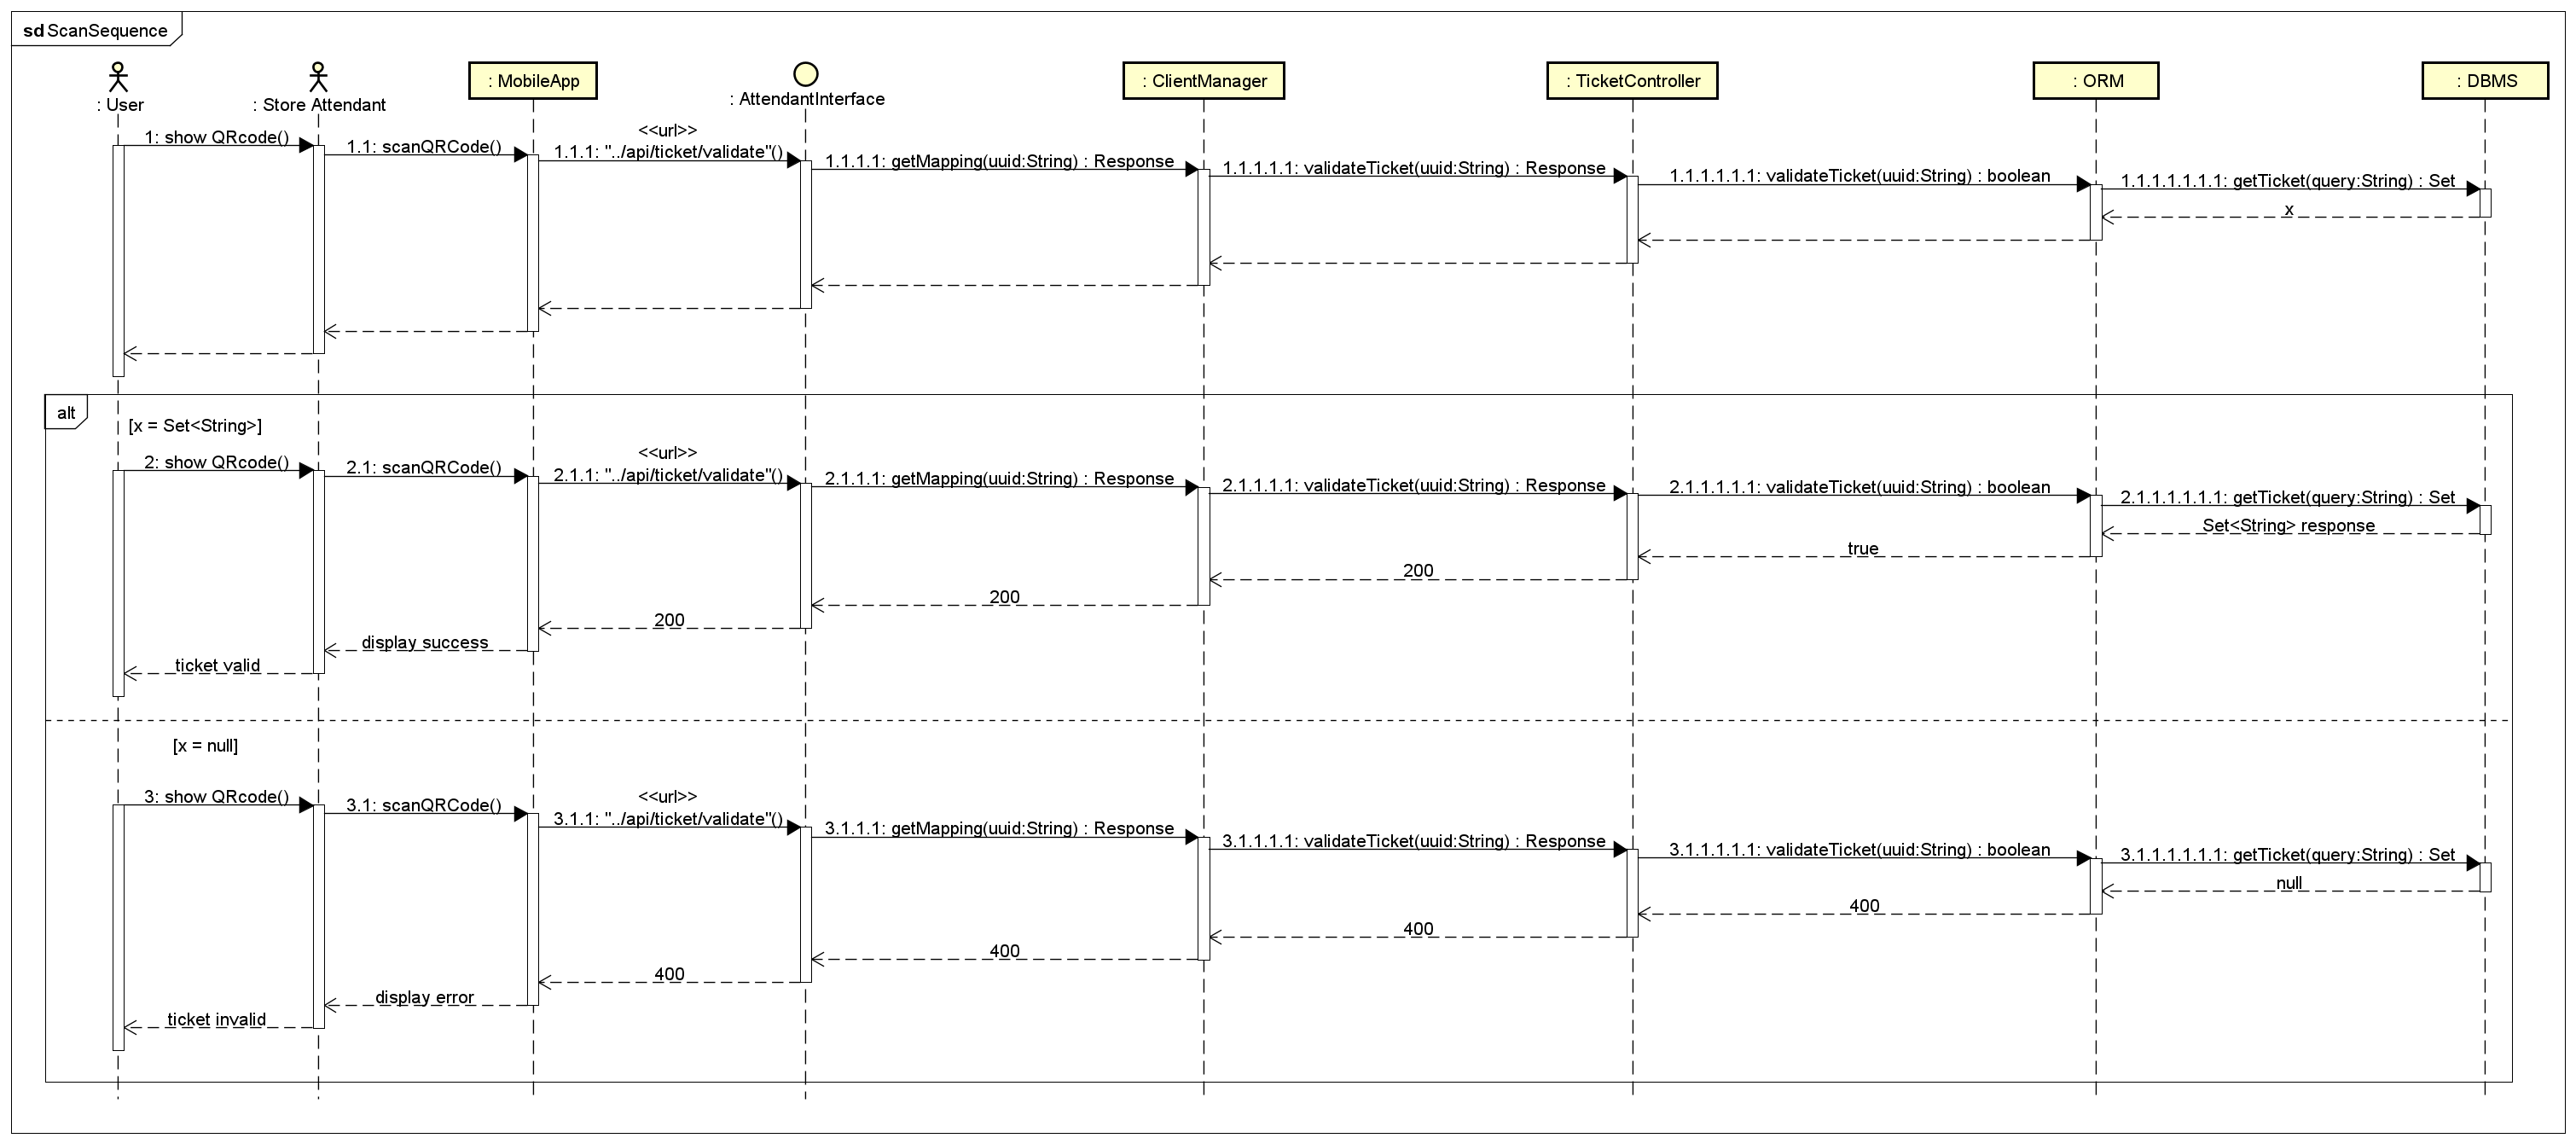
\includegraphics[width=\textwidth]{assets/Sequence-Diagram/ScanSequence.png}
    \end{center}
\end{figure}
The diagram above describes the process of scanning a customer's QR code.\\
The store attendant greets the customer, asking for the ticket's QR code, and opens the specific page.\\
After that they press the "scan" button and, using the webcam on the phone, scan the code; at this point the App sends the data to the ClientManager which forwards it to the QRCodeValidation component.\\
This last one interrogates the database to validate the code: if the query returns a value it means the code is valid, otherwise it sends an error.\\
If the validation is successful, the QRCodeValidation handler reports it to the ClientManager and to the App, where a message status is displayed.
\subsubsection{Modify time slots}
\begin{figure}[H]
    \begin{center}
        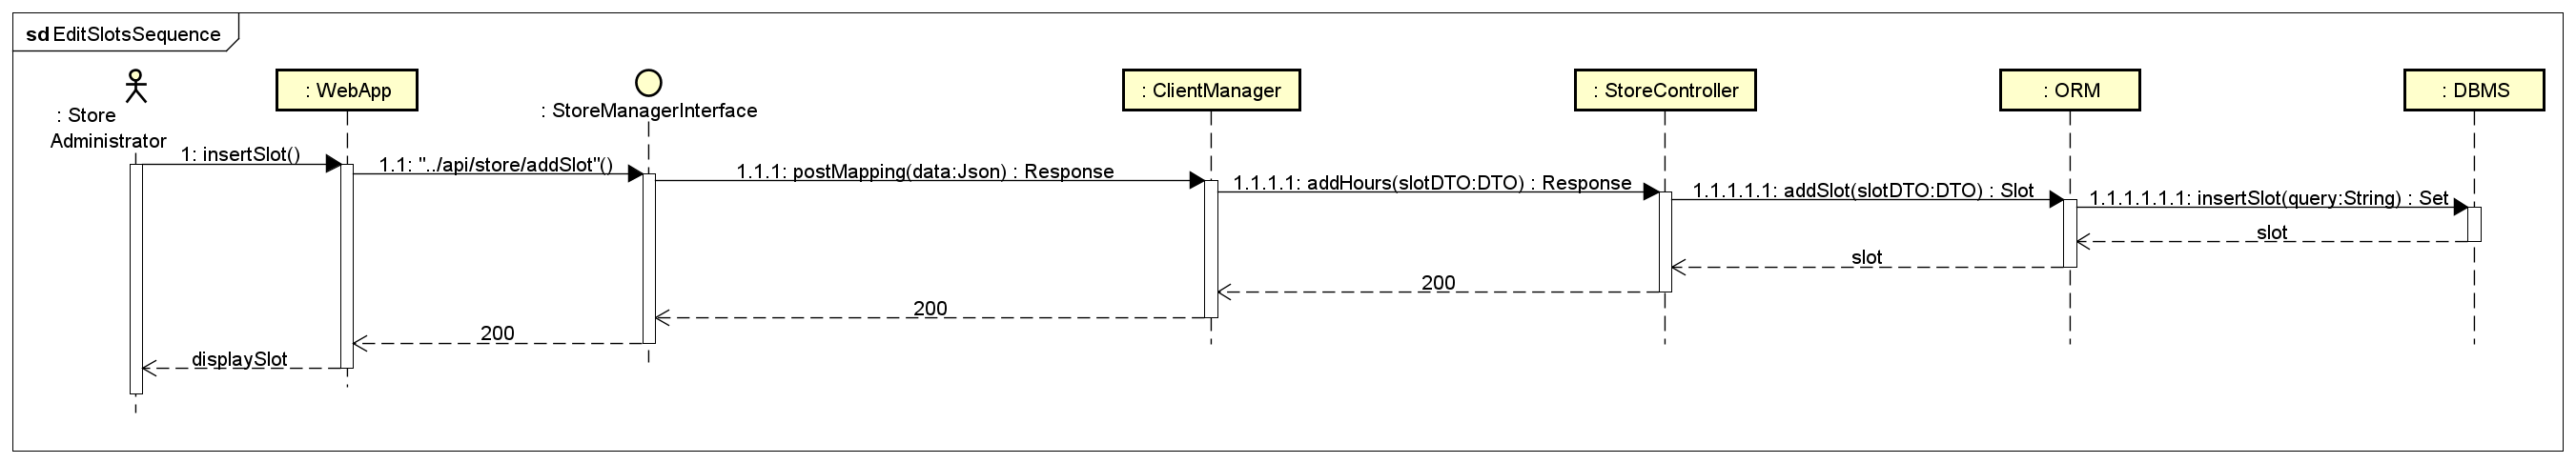
\includegraphics[width=\textwidth]{assets/Sequence-Diagram/EditSlotsSequence.png}
        \caption{Modify time slots sequence diagram}
    \end{center}
\end{figure}
This process is only available for the Store Administrator  and lets them edit the time slots of their store.\\
Through the appropriate page the Store Administrator edits the time slots of the store, this triggers a request from the App to the ClientManager and to the StoreManagement handler, which is responsible for updating the database with the new time slots and then reporting back to the ClientManager.\\
The App then displays a confirmation.
\subsection{Component Interfaces}
\begin{figure}[H]
    \begin{center}
        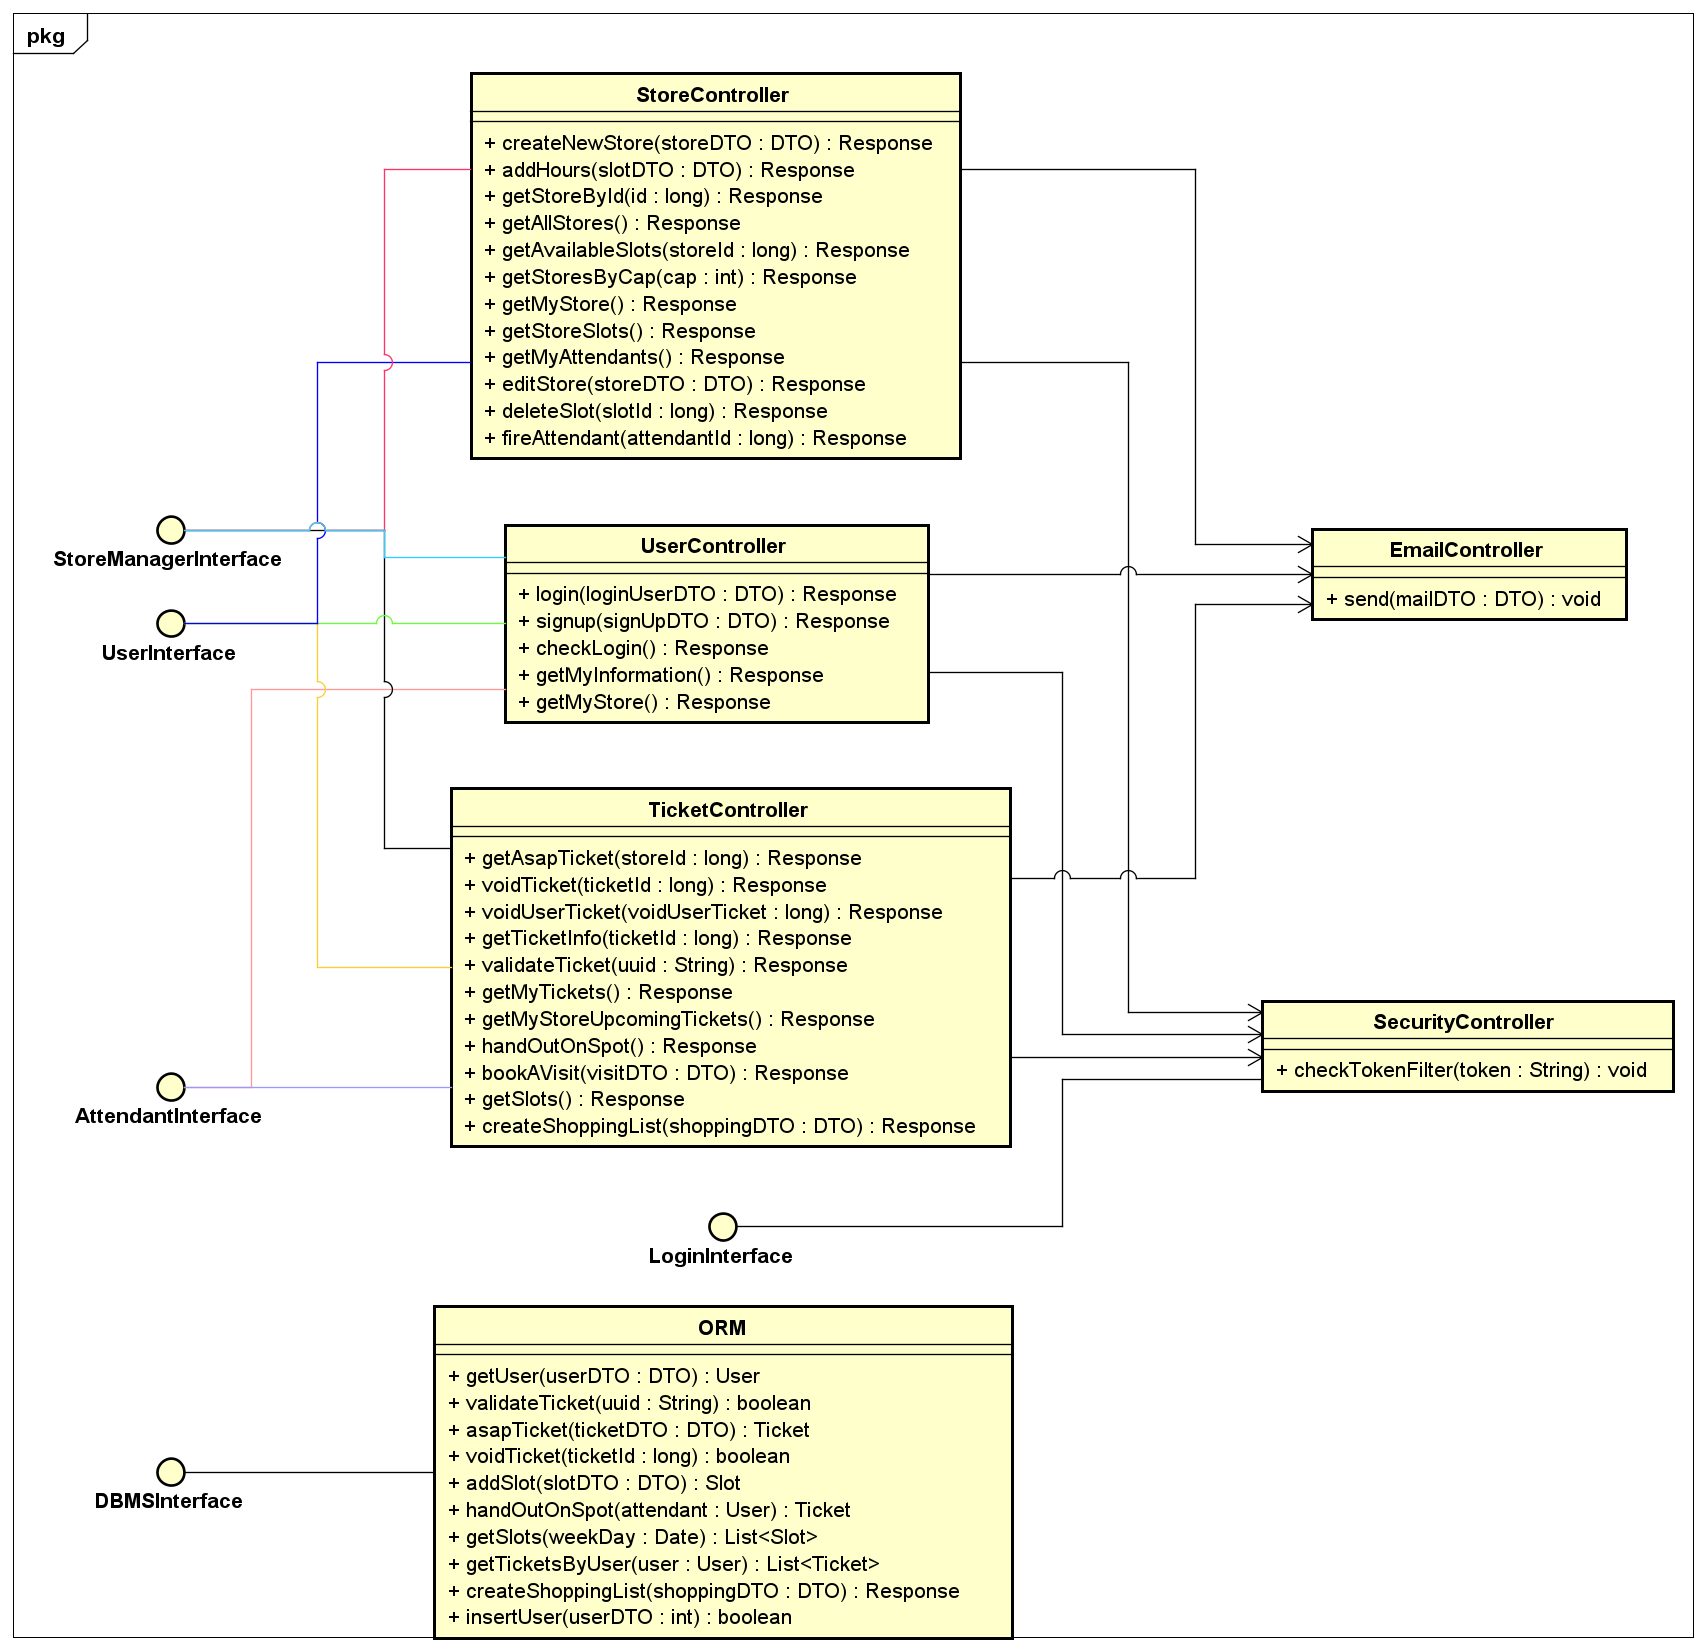
\includegraphics[scale=0.35]{assets/Interfaces/InterfacesDiagramUpdated.png}
        \caption{Interfaces Diagram}\label{interfaces_diagram}
    \end{center}
\end{figure}

The interfaces shown in figure\ref{interfaces_diagram} are the principal ones needed to make CLup run. The arrows represent the implementation classes of the interfaces.

Starting from the beginning, the \textbf{AccessInterface} is needed in order to hold the customer, store administrator and store attendant sign up and login processes. It is realized through two different controllers, called SignUpHandler and LoginHandler.

Then we can see the \textbf{UserInterface}, which main goal is to achieve user functionalities, such as the ASAP or the Reservation ones. It is realized by five different controllers, one for each functionality.
\begin{itemize}
    \item \textbf{ASAPController}: it manages the ASAP request sent by the user and returns a valid response with the booked slot or an error.
    \item \textbf{ReservationController}: same as above, but specifically designed for the \textit{Book a visit} functionality.
    \item \textbf{AlternativeSlotRecommender}: it calculates the best alternative slot and returns them back to the user.
    \item \textbf{QRCodeGenerator}: it manages the creation of the QRCode, when the user confirm the given (or chosen) slot.
    \item \textbf{Notification}: it manages the feature of periodic notification, sending to the user a message when it is almost time to go.
\end{itemize}

Then we have a store attendant interface, which main features are realized through different controllers.
\begin{itemize}
    \item \textbf{QRCodeValidationController}: it manages the process of QRCode validation at the entrances of the store. It receives the data sent from the attendant's mobile device and processes them in order to send him a response, which can be valid (so the customer can enter the store) or not.
    \item \textbf{GenerateOnSpot}: it manages the creation of a booking, held by the attendant from a proper desk. It simply receives the request from the attendant's device and computes a valid booking slot, sending it back to the attendant.
\end{itemize}

Finally, we have the \textbf{StoreAdminInterface}, which permits to each store manager to edit all the information about the shop. This job is done through different methods:
\begin{itemize}
    \item \underline{editStoreInfo}: this method receives as input some new store information (which are basically String objects) and a StoreAdministrator object. It edits the Store object in the database if only the manager is its administrator.
    \item \underline{editTimeslots}: this method receives as input the new timeslot information and, as before, a StoreAdministrator object. It edits the information in the database.
    \item \underline{editAttendants}: this last method receives some information about an attendant to be edited, and makes the change in the database.
\end{itemize}

\subsection{Logical Description of Data}
\begin{figure}[H]
    \begin{center}
        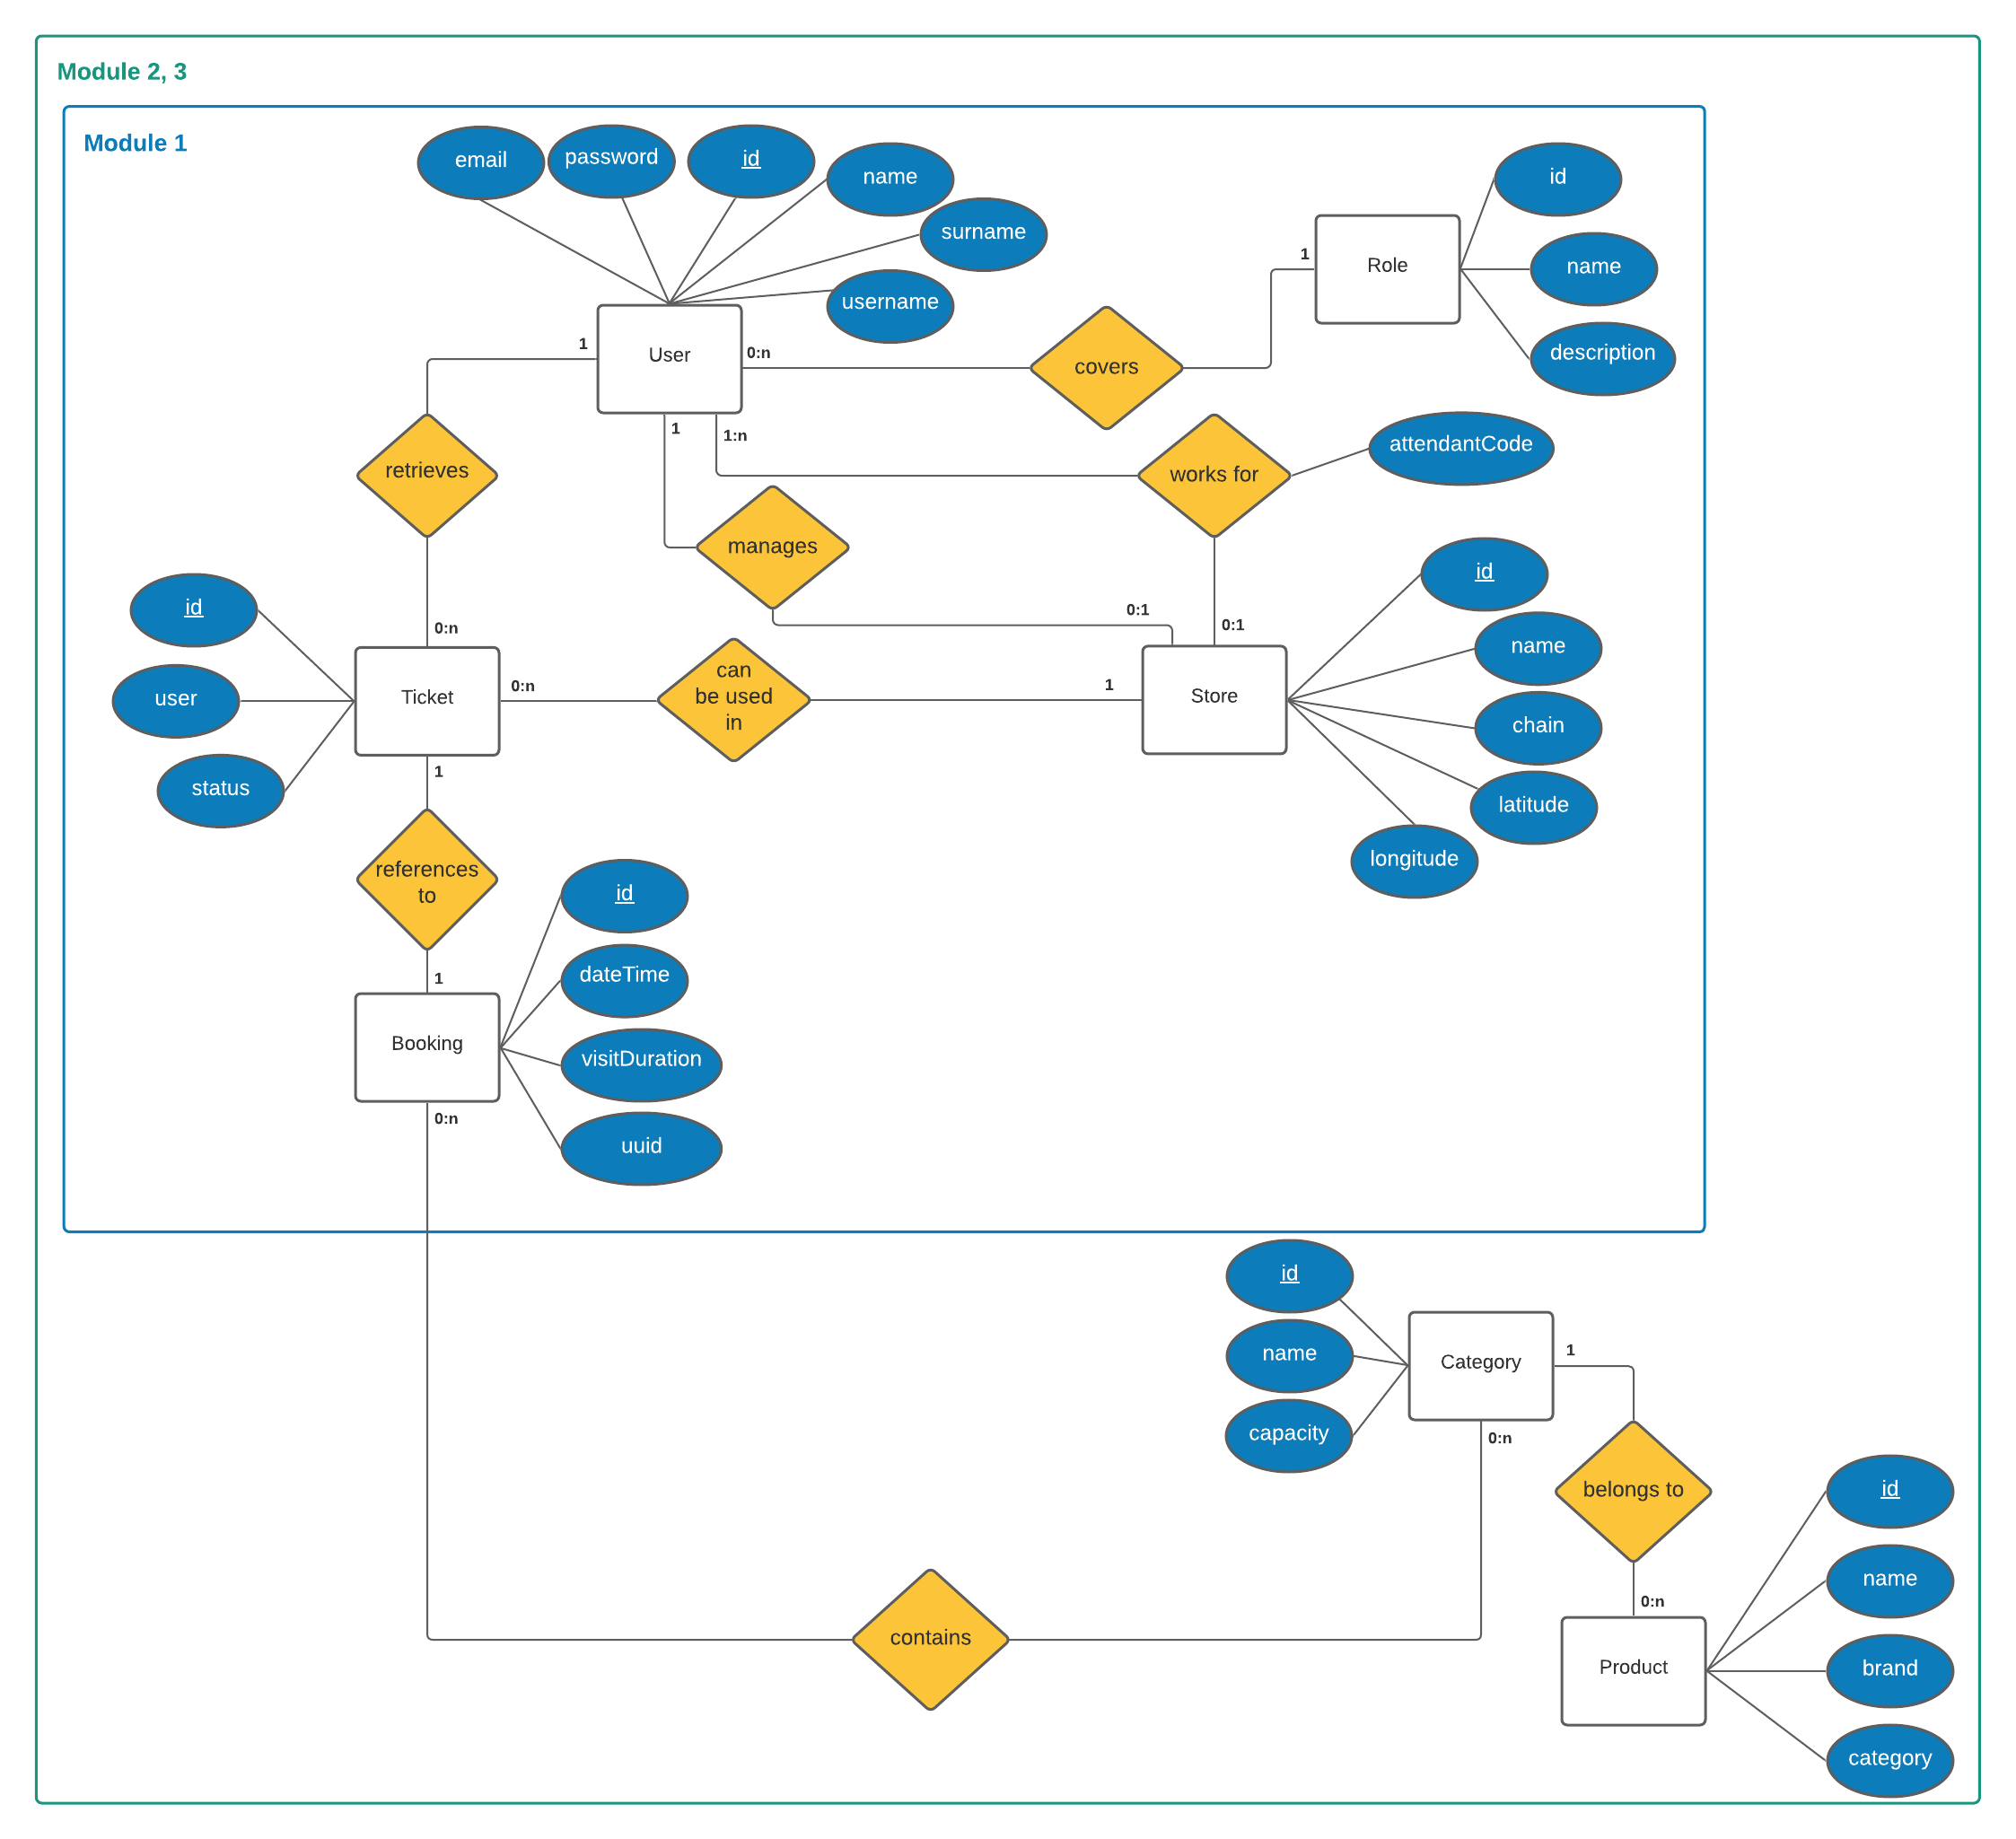
\includegraphics[width=\textwidth]{assets/Architectural-Design/ER.png}
        \caption{ER Diagram}\label{er_diagram}
    \end{center}
\end{figure}
The diagram in figure\ref{er_diagram} shows a logic representation of what kind of data is stored in the internal database of the S2B.

First of all, we can see the distinction in different modules (as s. 1.1 of RASD explains) and their respectively database structure in case of deployment on organization's servers. Of course, if the buyer chooses to remain on CLup official servers, the structure will remain the entire one, limiting the functionalities store by store.

The most important fact is that there are three different tables, each one for each customer type. In fact, since they contain different types of information, the most intuitive choice is the one of separating these types of data.

Then, we can see a table containing the list of all tickets, each of them associated to a specific store and (in case of \textit{Reservation} functionality) to a specific booking.

Finally, a booking can contain a list of categories, each one with a set of product inside it.

Looking at the relations, we can see that there is a \textit{bridge table} between Booking and Category, which associates a set of categories to one or more bookings. This association is used if a customer decides to insert a list of product in a reservation request.

\subsection{Architectural Style and Patterns}
\subsubsection{Four-tiered architecture}
We chose this architecture for many reasons:
\begin{itemize}
    \item \textbf{Flexibility:} Once the interfaces of the S2B are defined, then the interior logic is dependent from outside. This fact implicates that each module can be improved without changing all the others.
    \item \textbf{Scalability:} an application divided on several tiers guarantees that the approach of scaling the architecture is adopted only for the most critical components. The result obtained maximizes the performance but also minimizes the costs.
    \item \textbf{Load Distribution:} the presence of several application servers, preceded by a load balancer, guarantees an acceptable division of requests. Otherwise, the presence of a single node means that node can become over-requested, sending the entire system down.
\end{itemize}

\subsubsection{RESTful Architecture}
\label{REST}
The restful application will be adopted both on web and mobile side. This architecture is based on the stateless principle, in which the server does not contain any information about the state of client, that is managed directly on client side.

An useful property of this architecture is the \textit{code on demand} one, which permits sending some code snippets from the server to the client, and then make the client executing them locally (usually in the web browser). This behavior guarantees less computational load on the server and also a dynamic attitude of the service.

The application is then intended to be developed through \textit{client side scripting}, which means that all requests and update of the page are made on client side. This behavior also improves the user experience, and prevent refreshing the page each time an action is made.

\subsubsection{Model View Controller (MVC)}
Model–view–controller (usually known as MVC) is a software design pattern commonly used for developing user interfaces that divides the related program logic into three interconnected elements. This is done to separate internal representations of information from the ways information is presented to and accepted from the user.

These three components are:
\begin{itemize}
    \item \textbf{Model:} the central component of the pattern. It is the application's dynamic data structure, independent of the user interface. It directly manages the data, logic and rules of the application.
    \item \textbf{View:} any representation of information such as a chart, diagram or table. Multiple views of the same information are possible, such as a bar chart for management and a tabular view for accountants.
    \item \textbf{Controller:} accepts input and converts it to commands for the model or view.
\end{itemize}

\subsection{Other Design Decision}
\subsubsection{Scale-Out}
This method consists of cloning the nodes in which we expect to have a bottleneck in order to increase the general system scalability.

This choice leads to a higher deployment effort but also to a lower hardware upgrade cost when the limits are reached. In conclusion, the scale-out is a preferable road.

Once split, the system requires a load balancer in order to correctly redirects the incoming requests to the node with the lowest workload.

\subsubsection{Thin client and fat server}
This architecture consists of keeping as low information as possible on client side. It means that the business logic resides only on server side.

The minimum requirement of this choice is a stable connection between the parts; otherwise the application would not work as expected.

Of course, the main advantage of choosing this implementation style is that the client machine is not required to have an high computational power.

\subsubsection{Adoption of IdP Providers}
We decided to adopt some external IdP providers (such as Facebook, Google, etc.) in order to simplify the process of user registration, without asking him any additional information.

This service is based on the providers API, which will communicate with our service in order to provide the necessary information (such as an email address).

\section{User Interface Design}
The aim of this section is to show the design of the main screens of the User app, describing the flow of the main functionalities for which the application was intended. The flow is created according to specific and illustrated input of the final user \\
\textbf{Please note that} we used some mockups presented in the RASD but more mocks have been created and added to this part in order to better clarify the user experience. In addition, we chose to show only screenshot of the mobile application because in our opinion Users would interact mostly with it. We want to remember that the application will work also on web browsers, but the design and the interfaces of the web app will derive from these ones, and the accurate design choices of them are out of the aim of this project. \\

\subsection{User Mobile Interface}
\begin{center}
    \begin{figure}[H]
        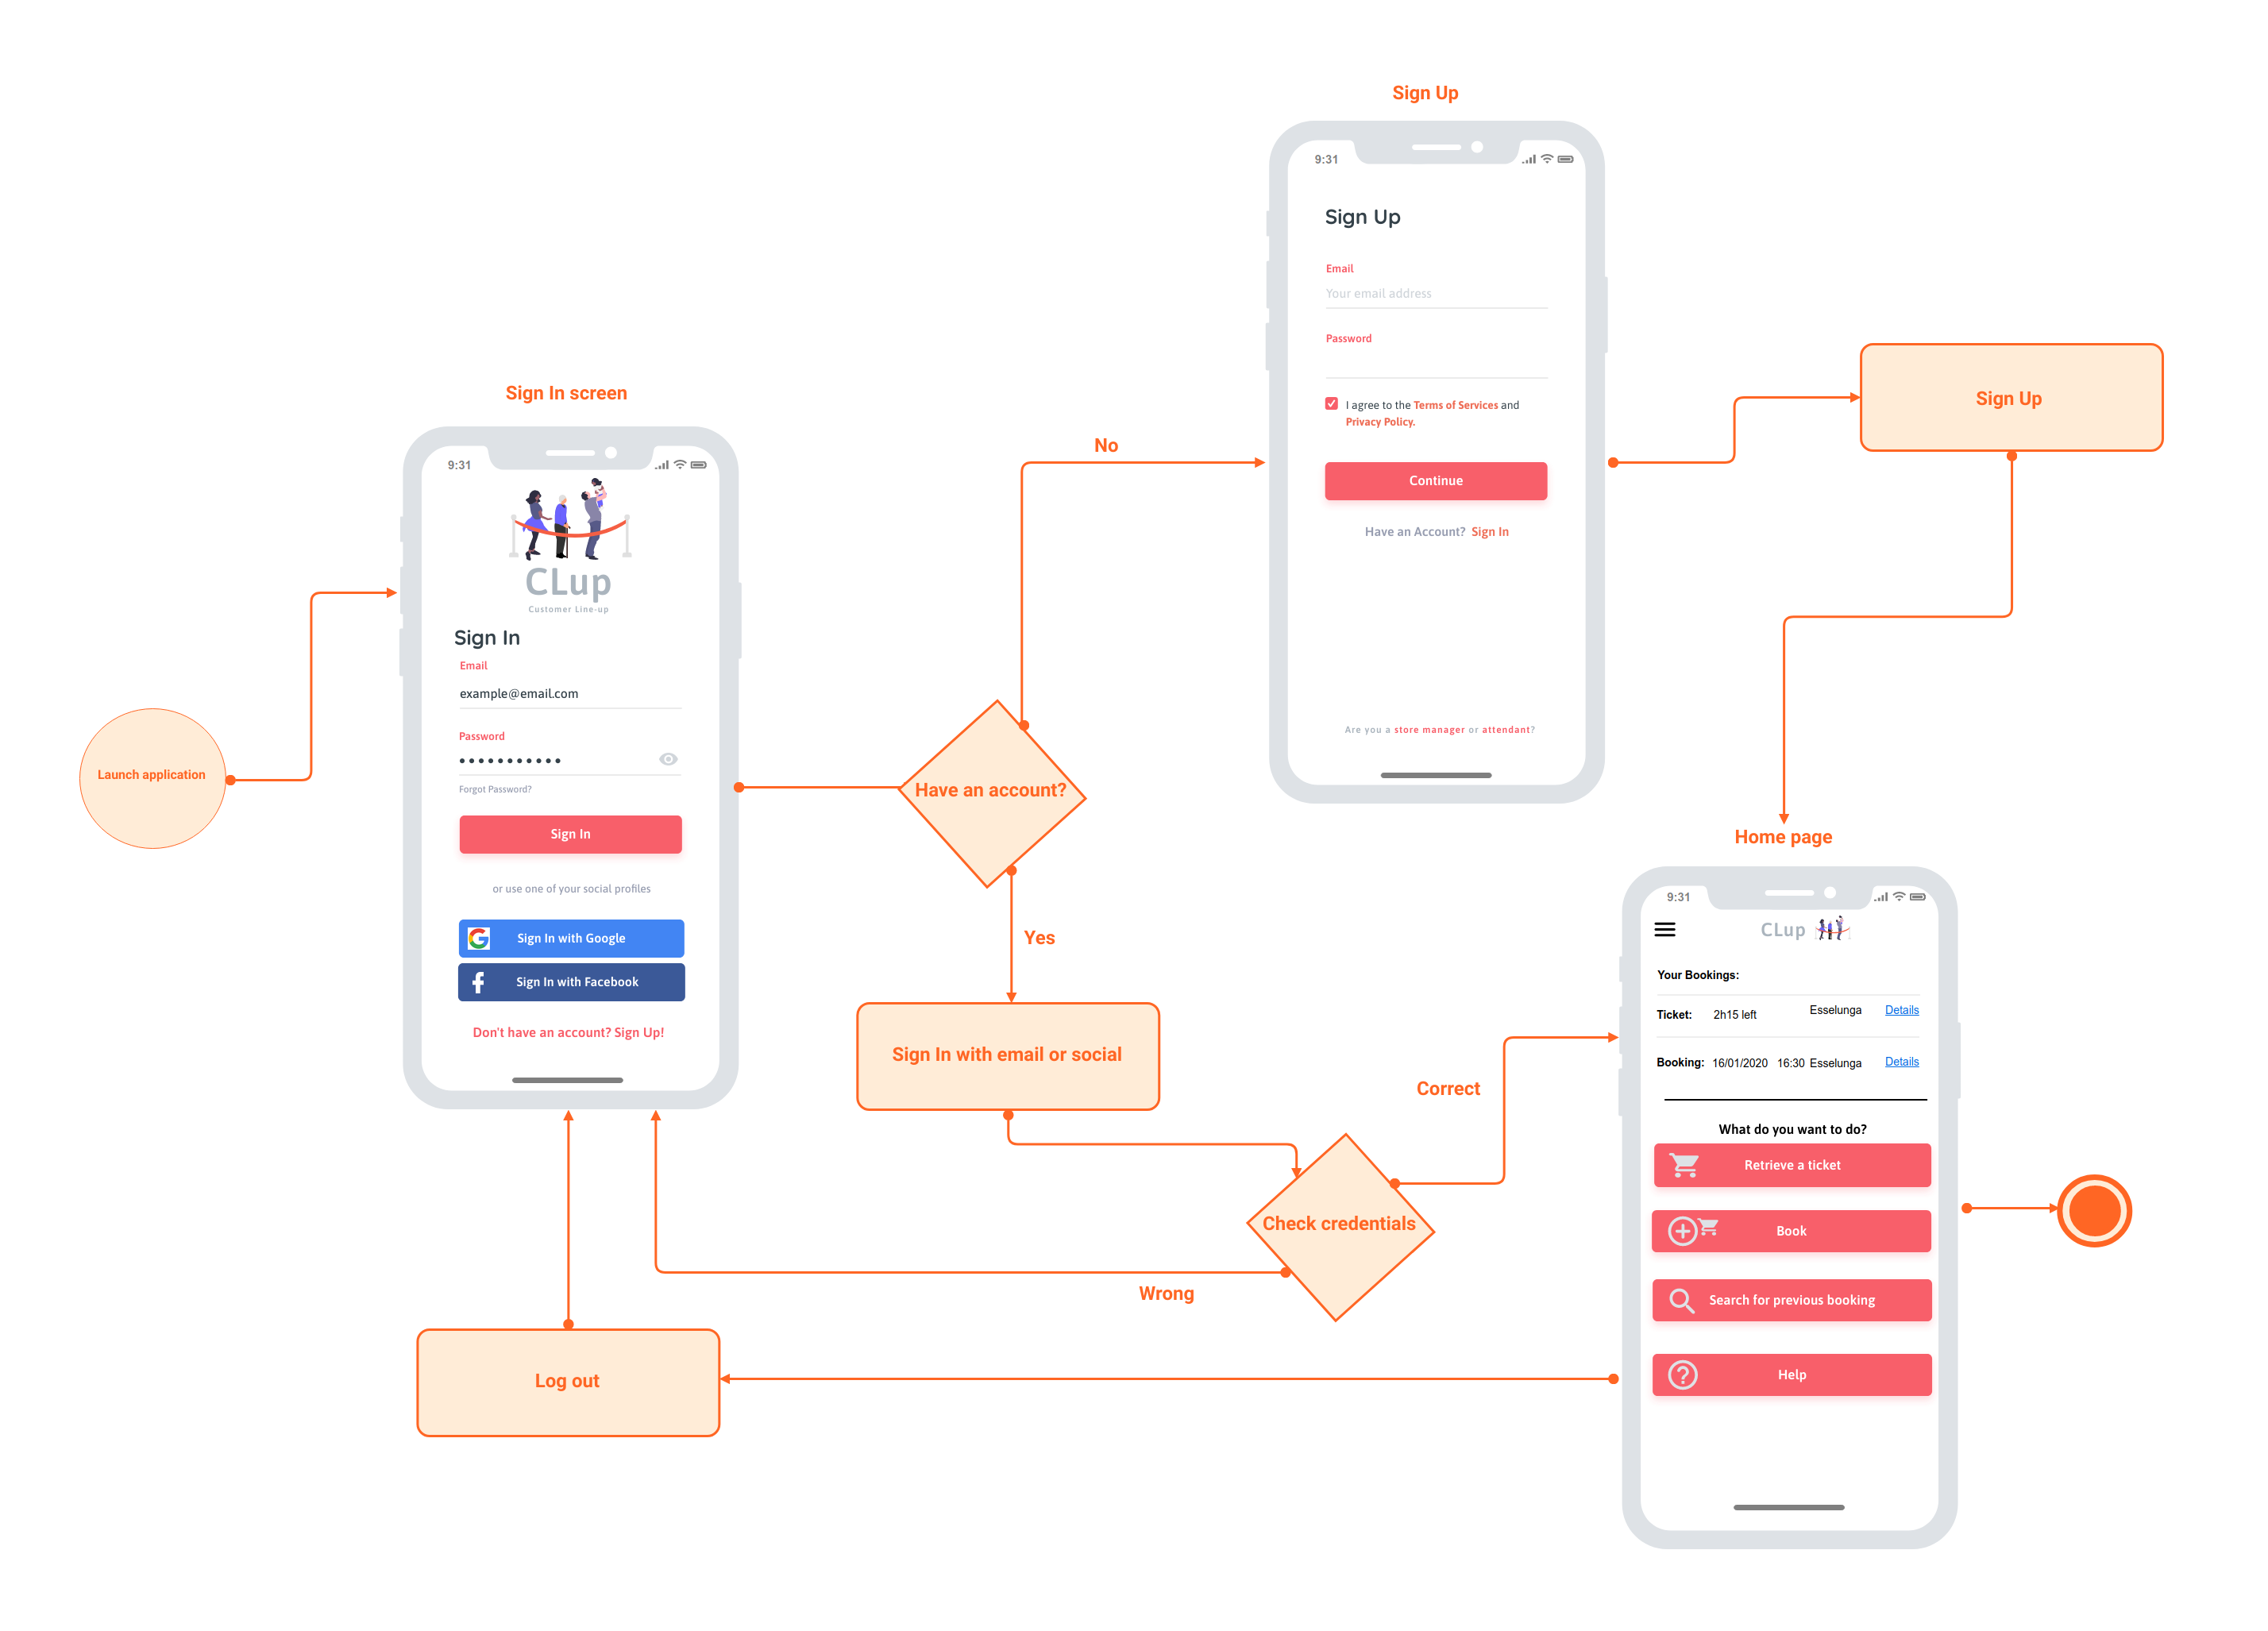
\includegraphics[width=\textwidth]{assets/User-Interface-Design/SignIn_SingUp_User.png}
        \caption{Sign Up \& Sign In}
    \end{figure}
\end{center}

\begin{center}
    \begin{figure}[H]
        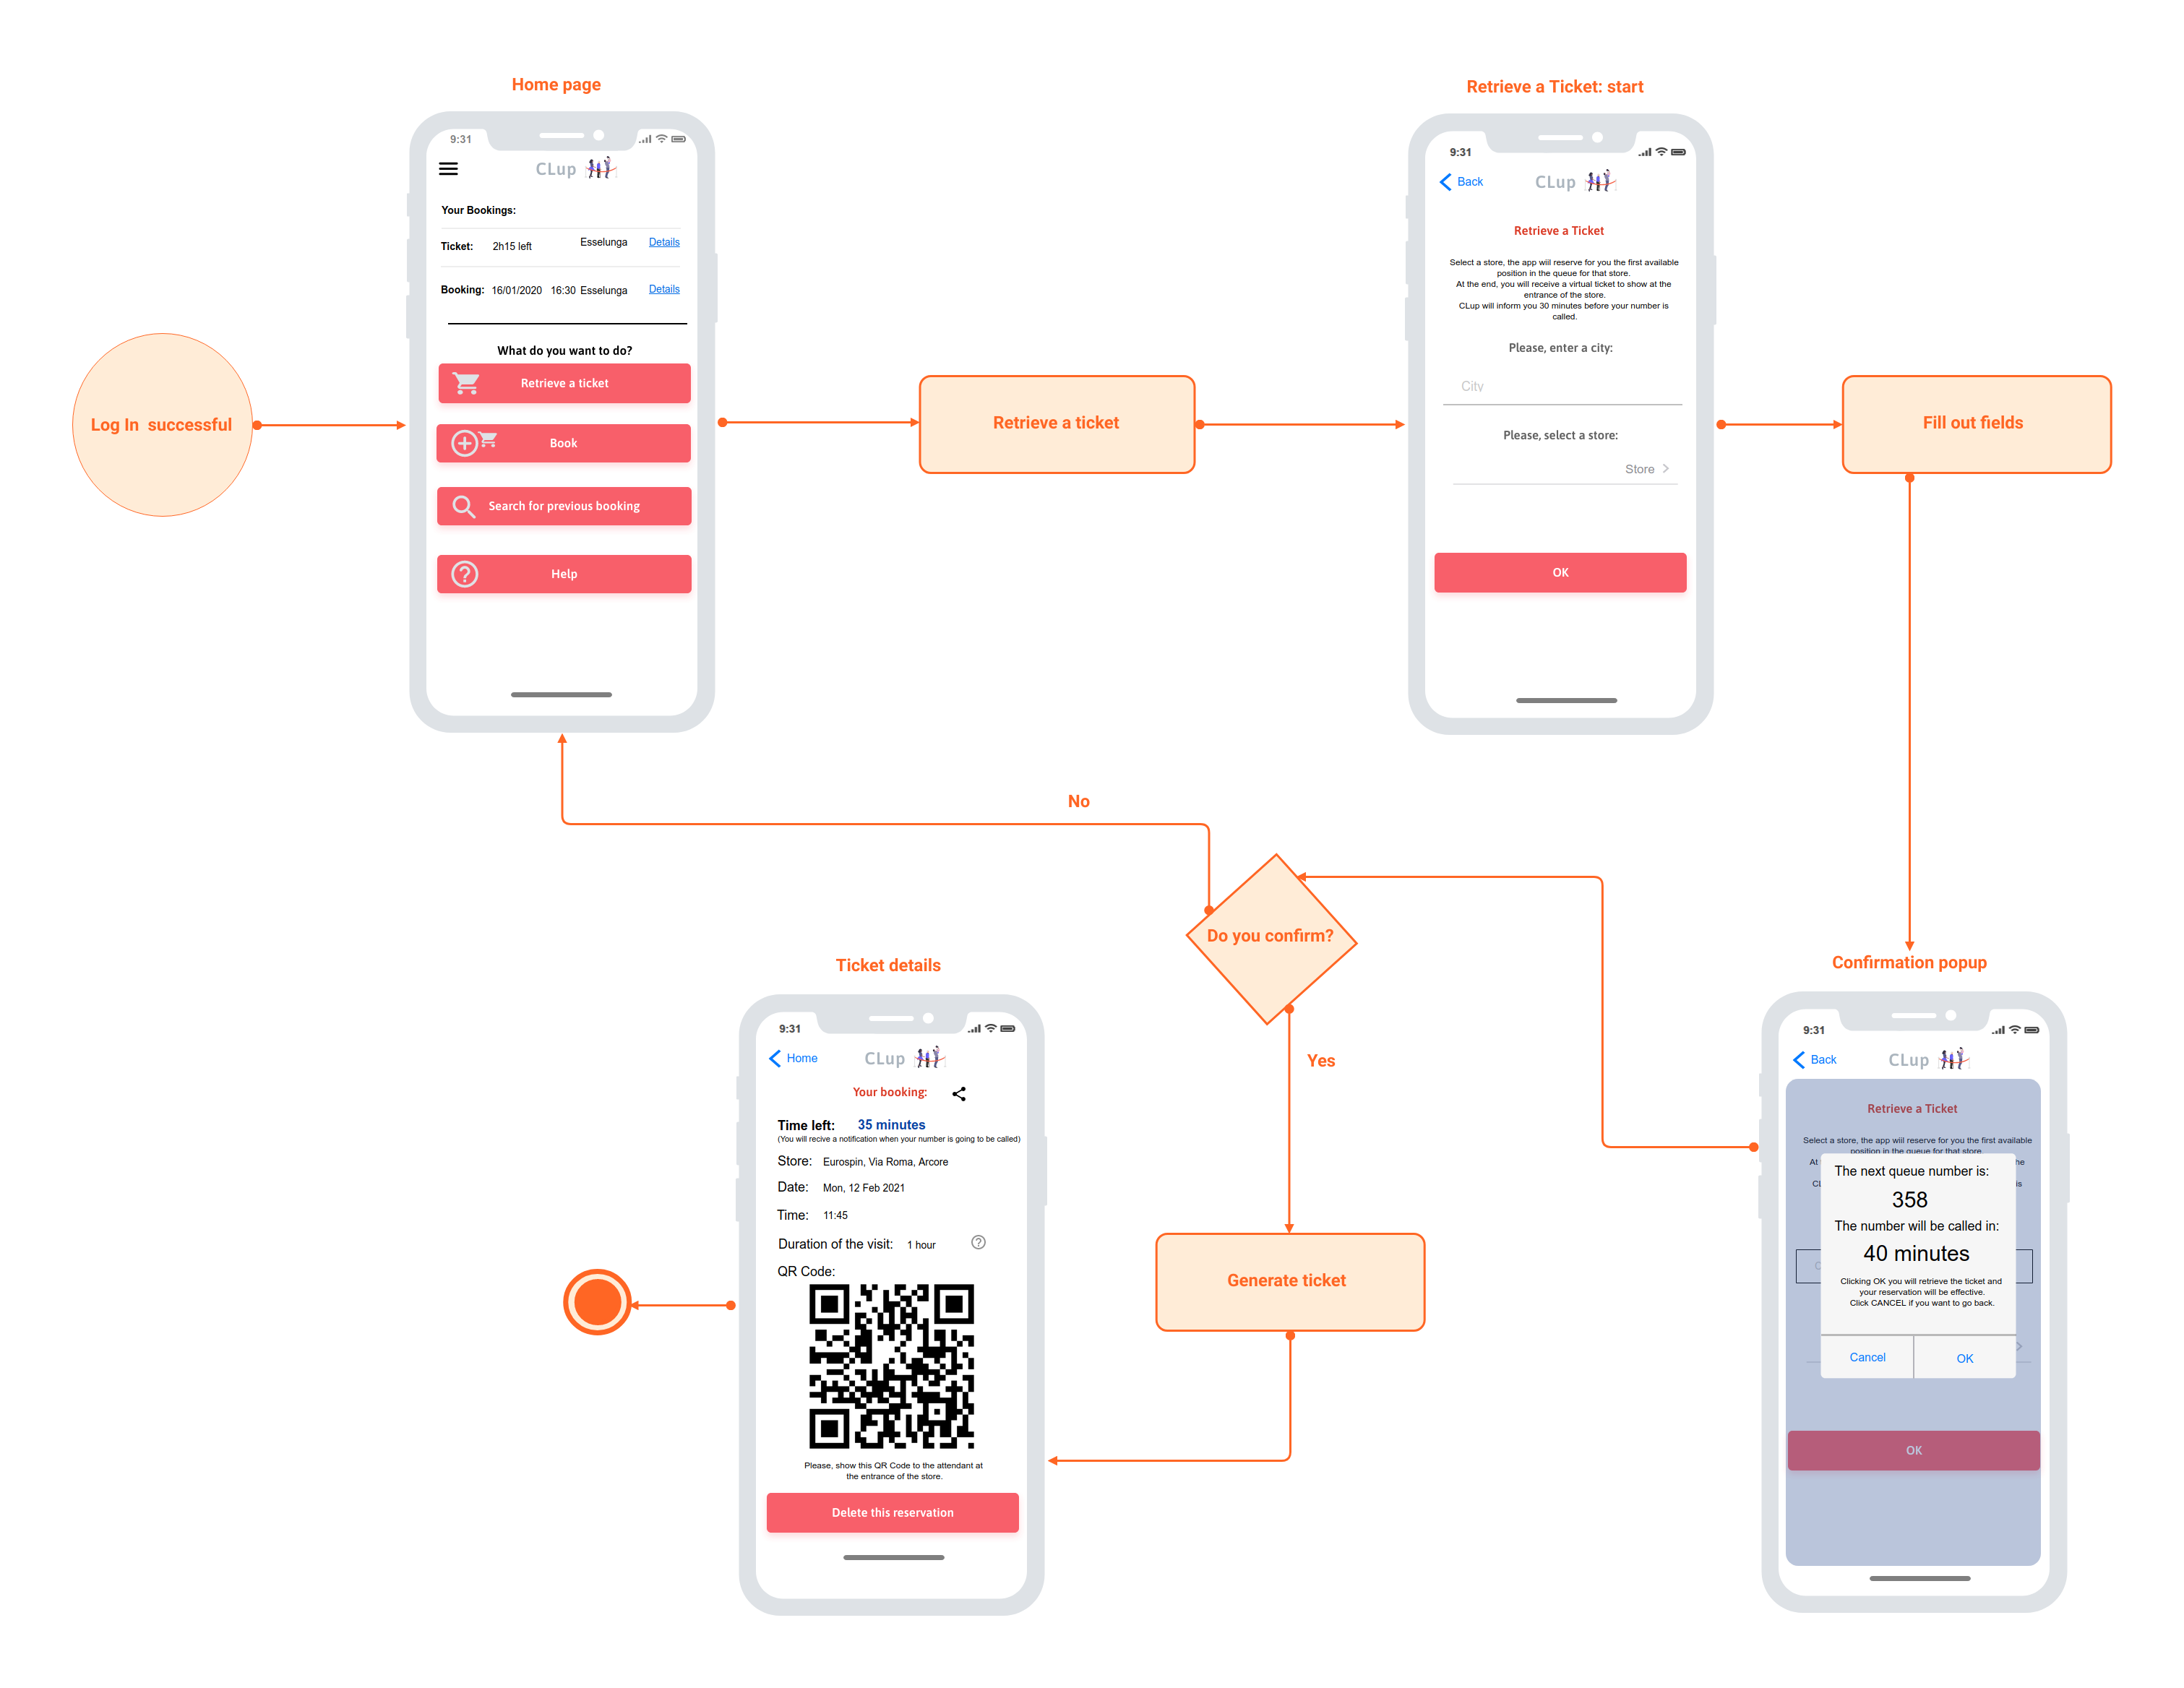
\includegraphics[width=\textwidth]{assets/User-Interface-Design/retrieve_a_ticket_User.png}
        \caption{ASAP functionality}
    \end{figure}
\end{center}

\begin{center}
    \begin{figure}[H]
        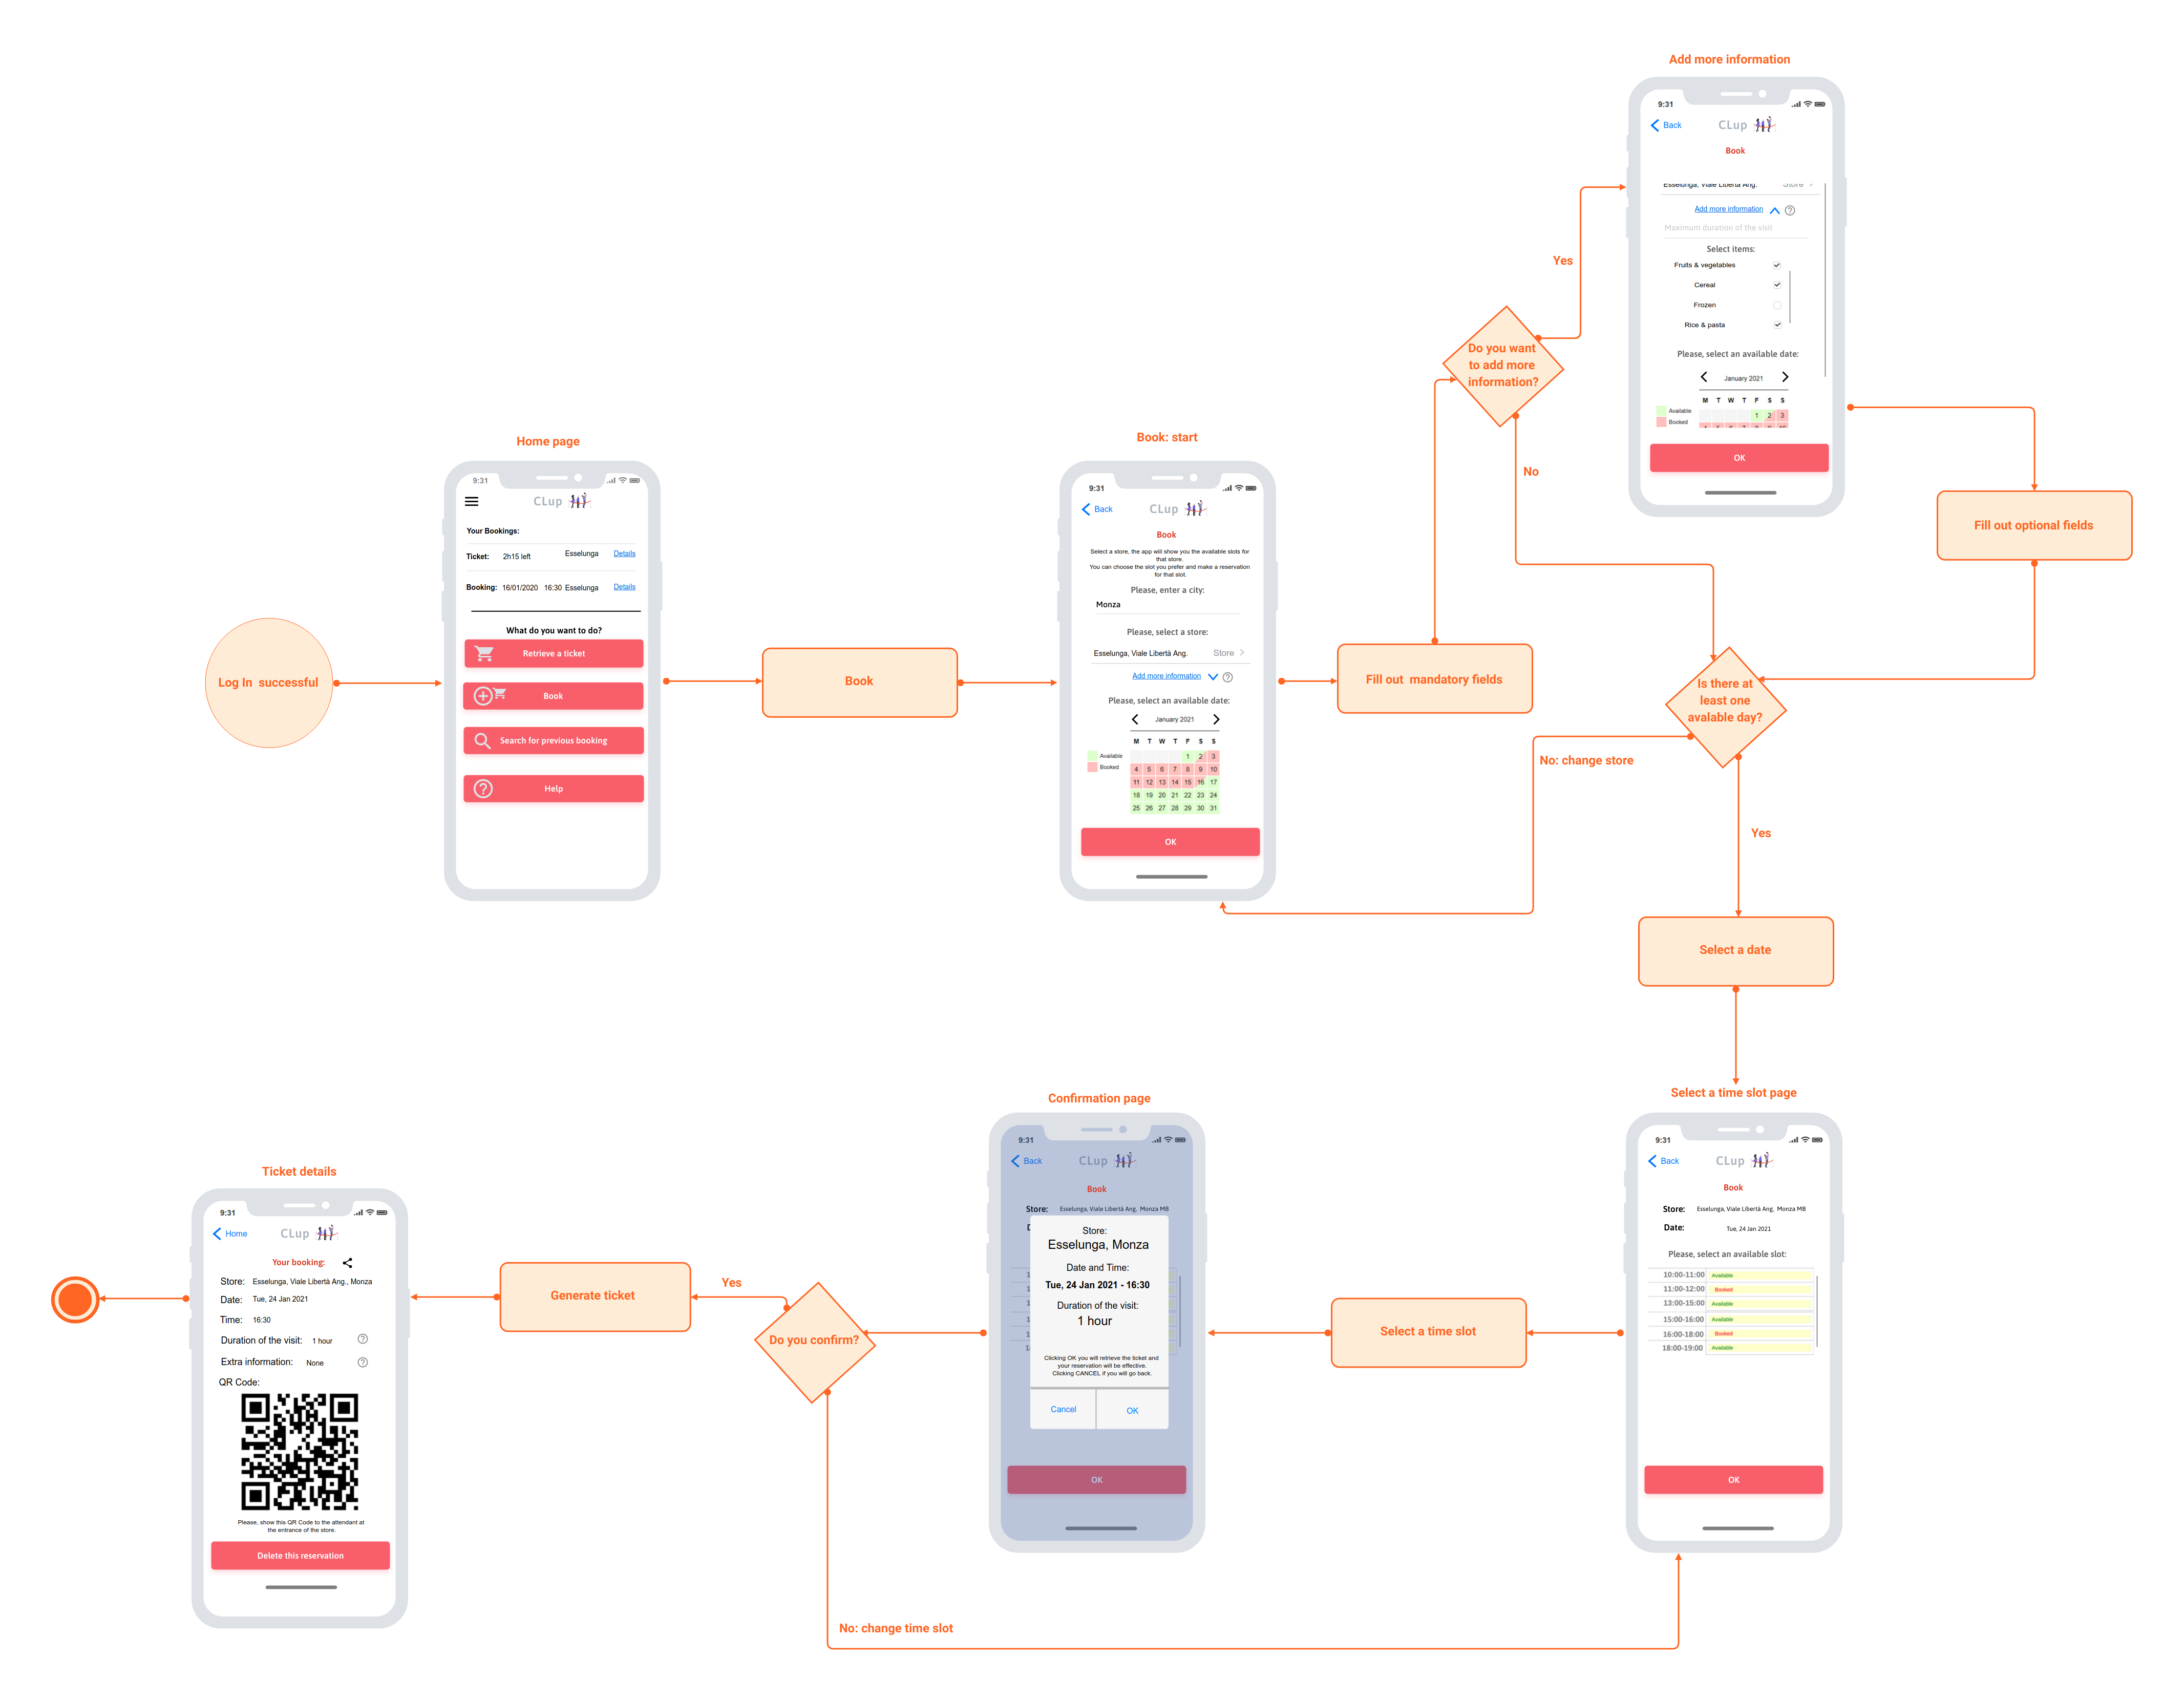
\includegraphics[width=500pt]{assets/User-Interface-Design/book_a_visit_User.png}
        \caption{Reservation functionality}
    \end{figure}
\end{center}

\begin{center}
    \begin{figure}[H]
        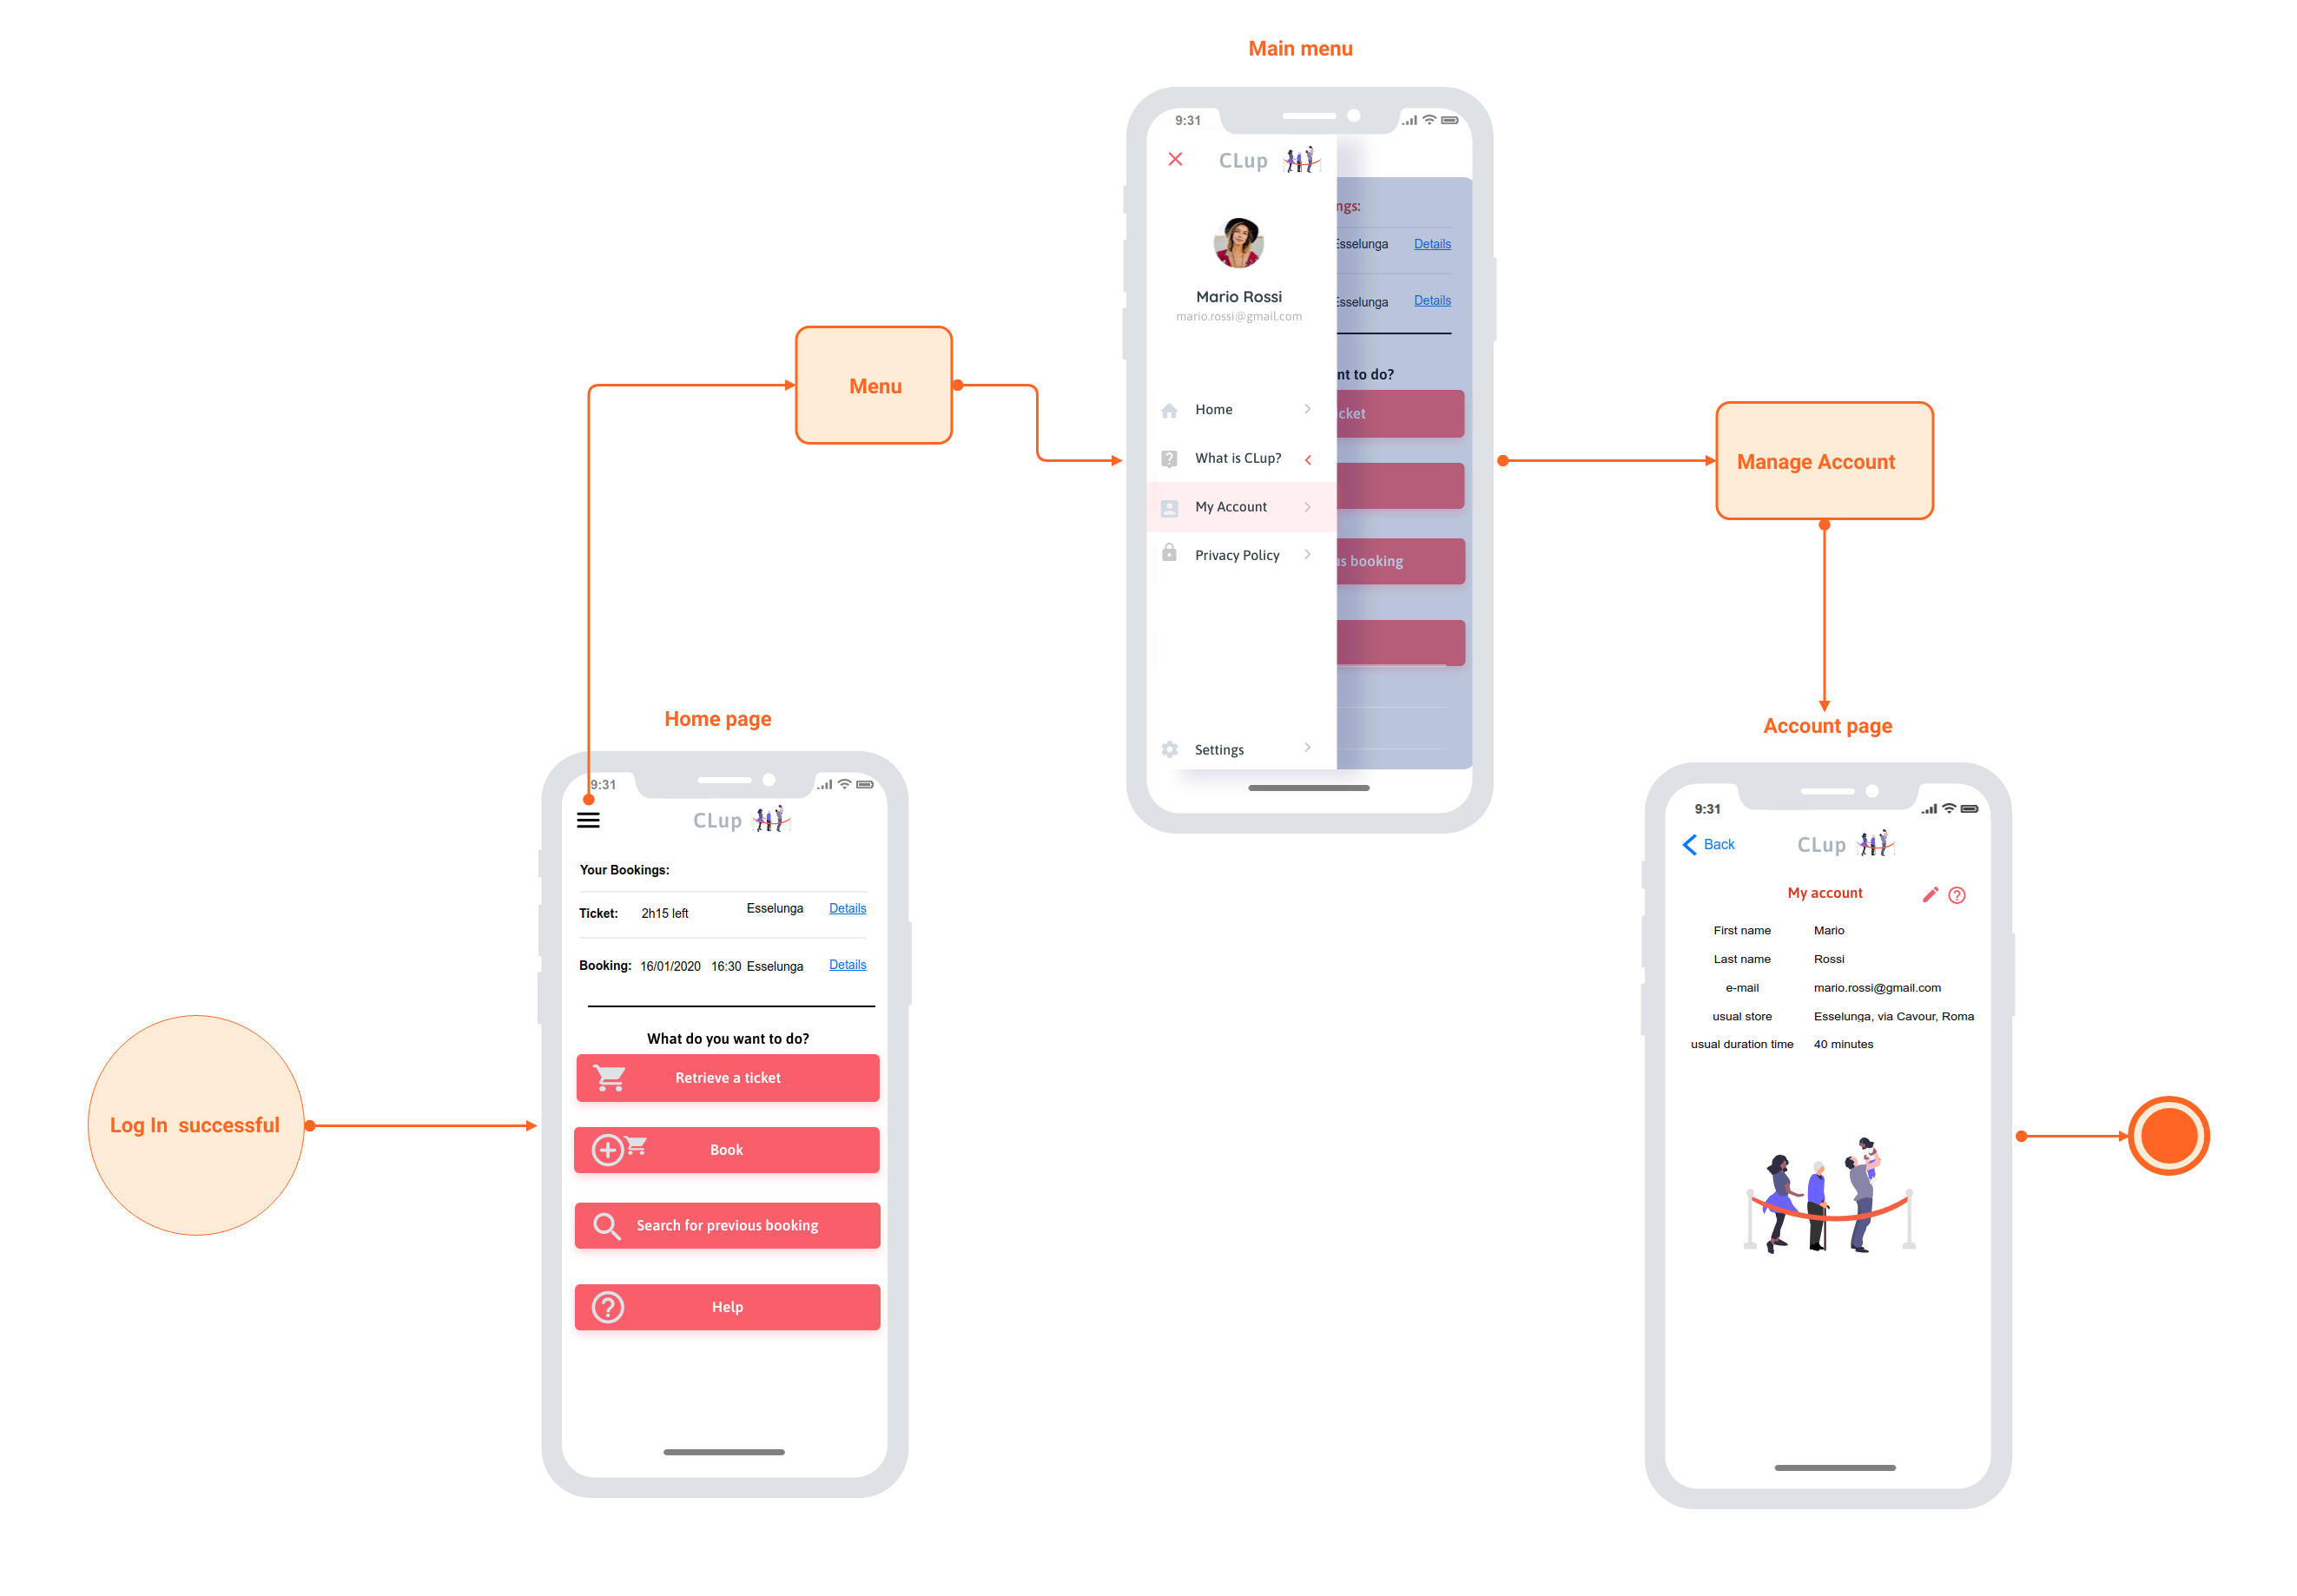
\includegraphics[width=\textwidth]{assets/User-Interface-Design/account.png}
        \caption{Manage account}
    \end{figure}
\end{center}

\subsection{Attendant Mobile Interface}
\begin{center}
    \begin{figure}[H]
        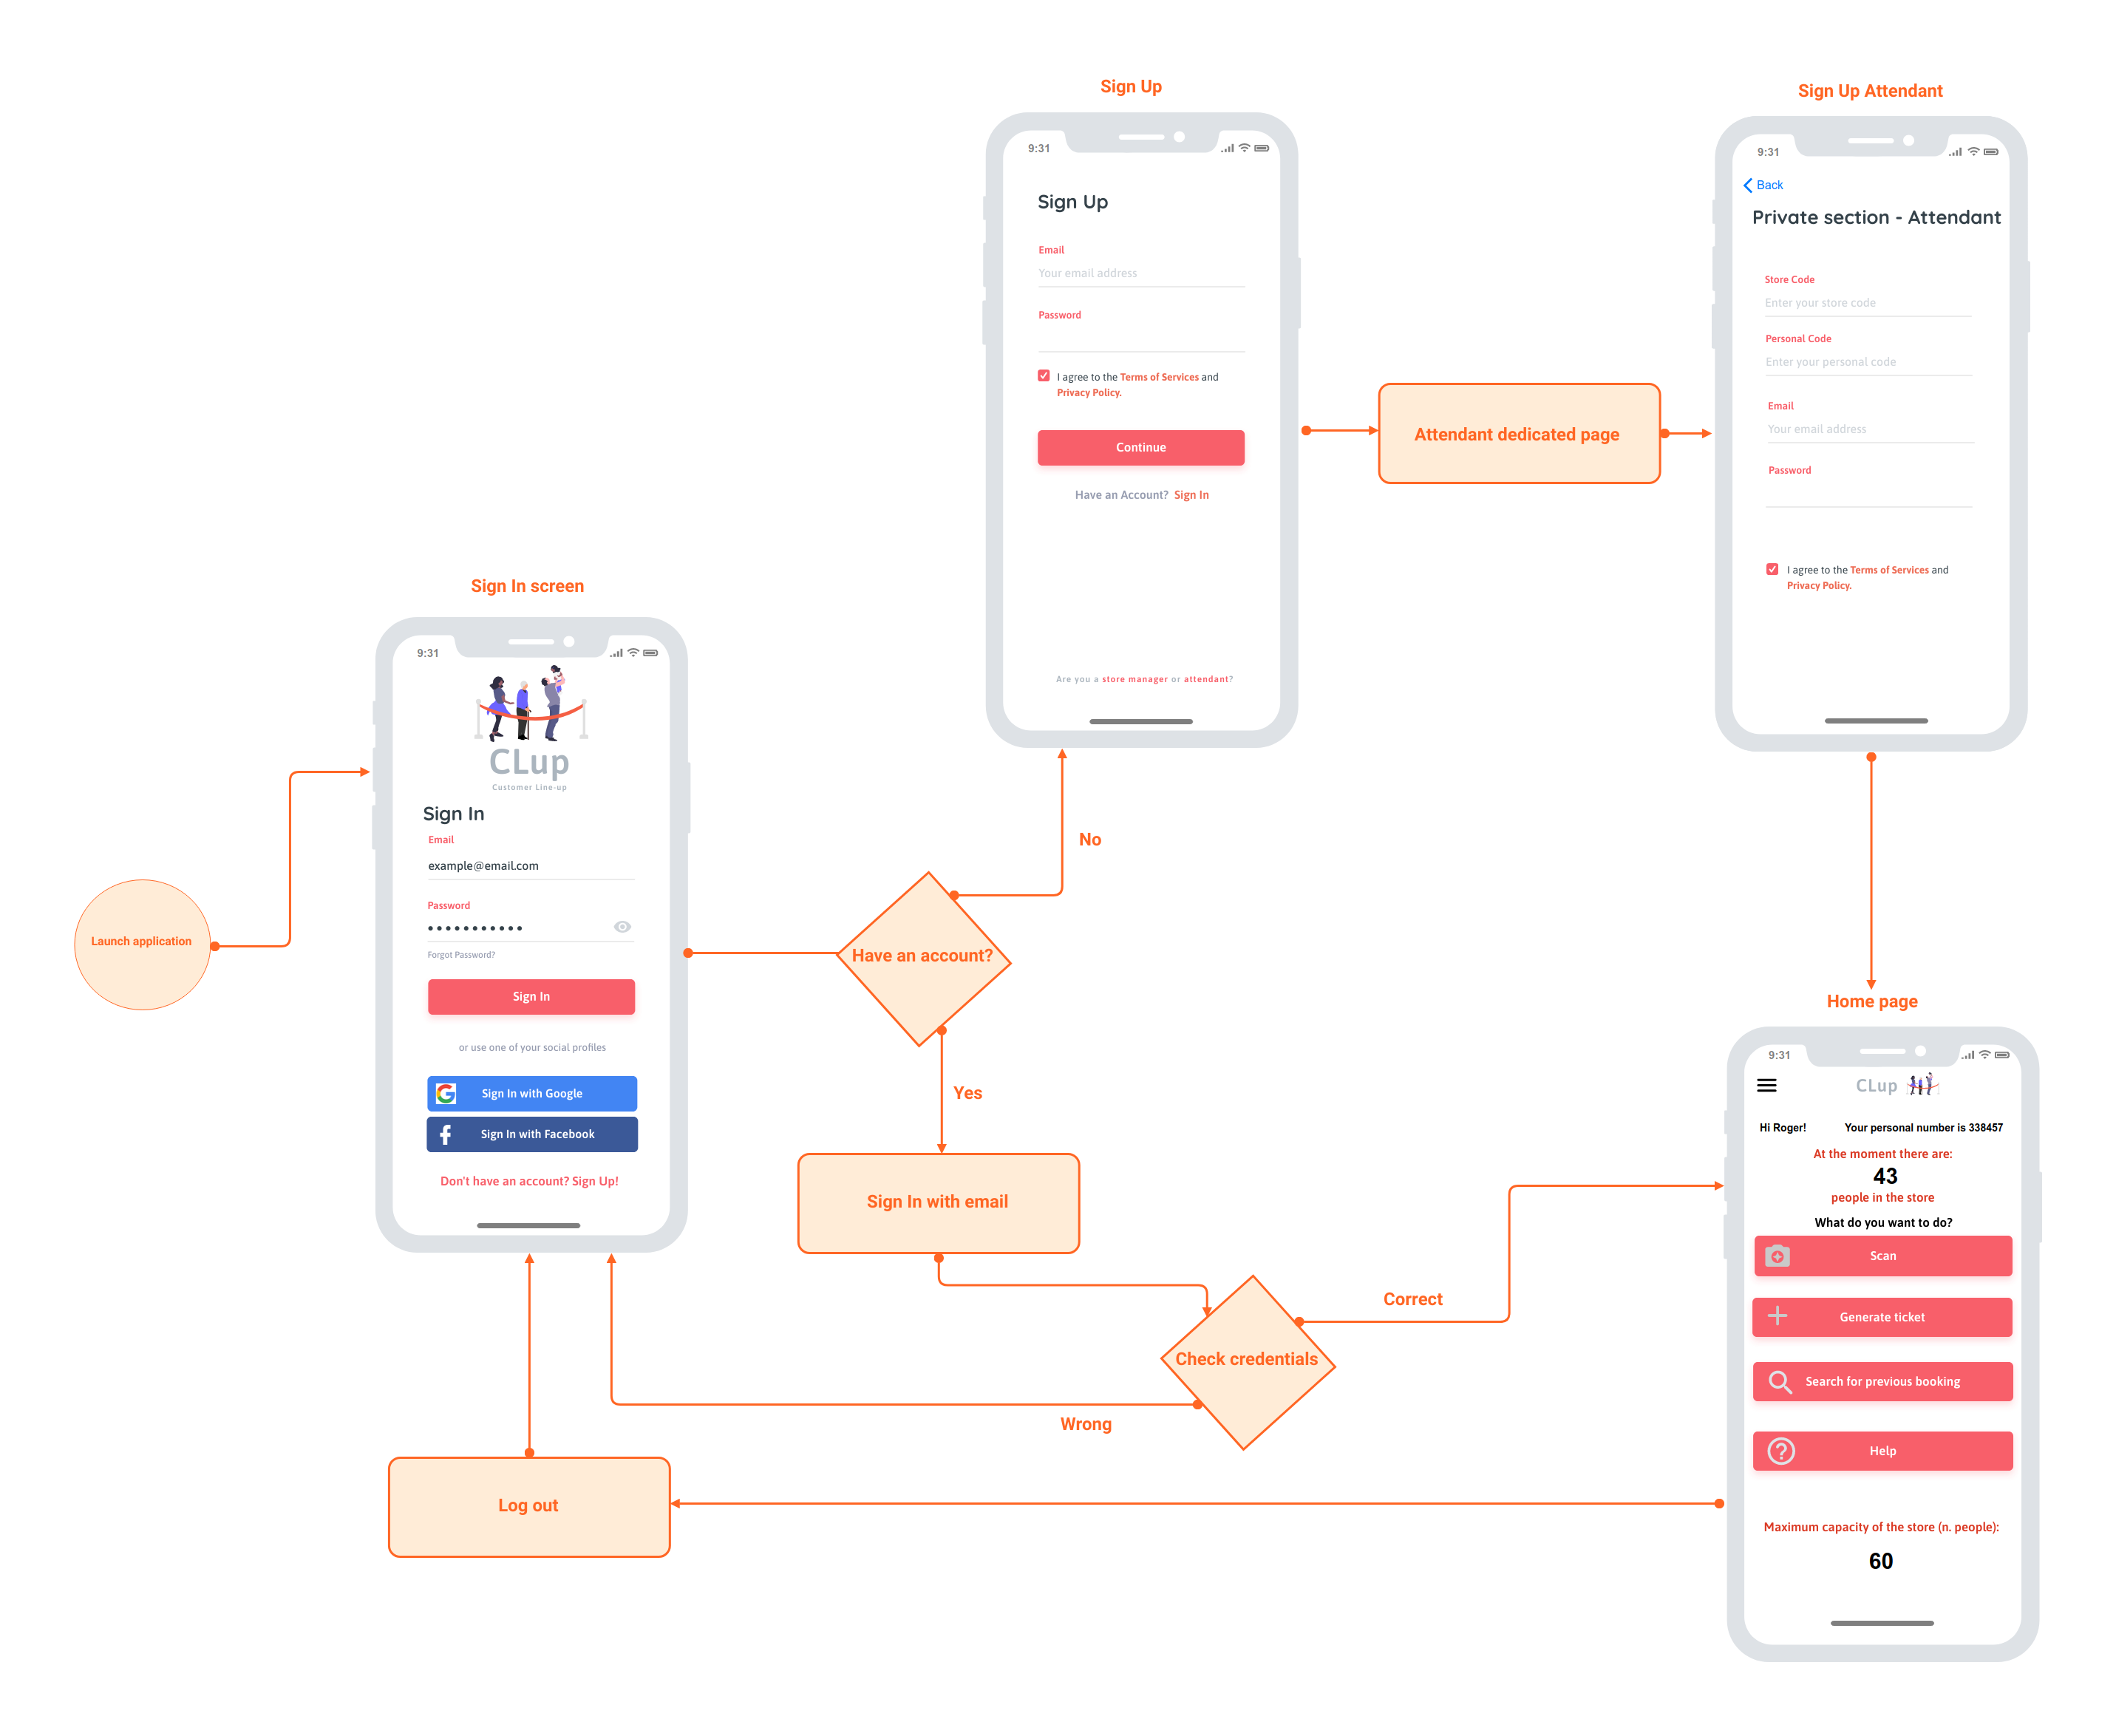
\includegraphics[width=\textwidth]{assets/User-Interface-Design/sign_up_attendant.png}
        \caption{Sign Up \& Sign In}
    \end{figure}
\end{center}

\begin{center}
    \begin{figure}[H]
        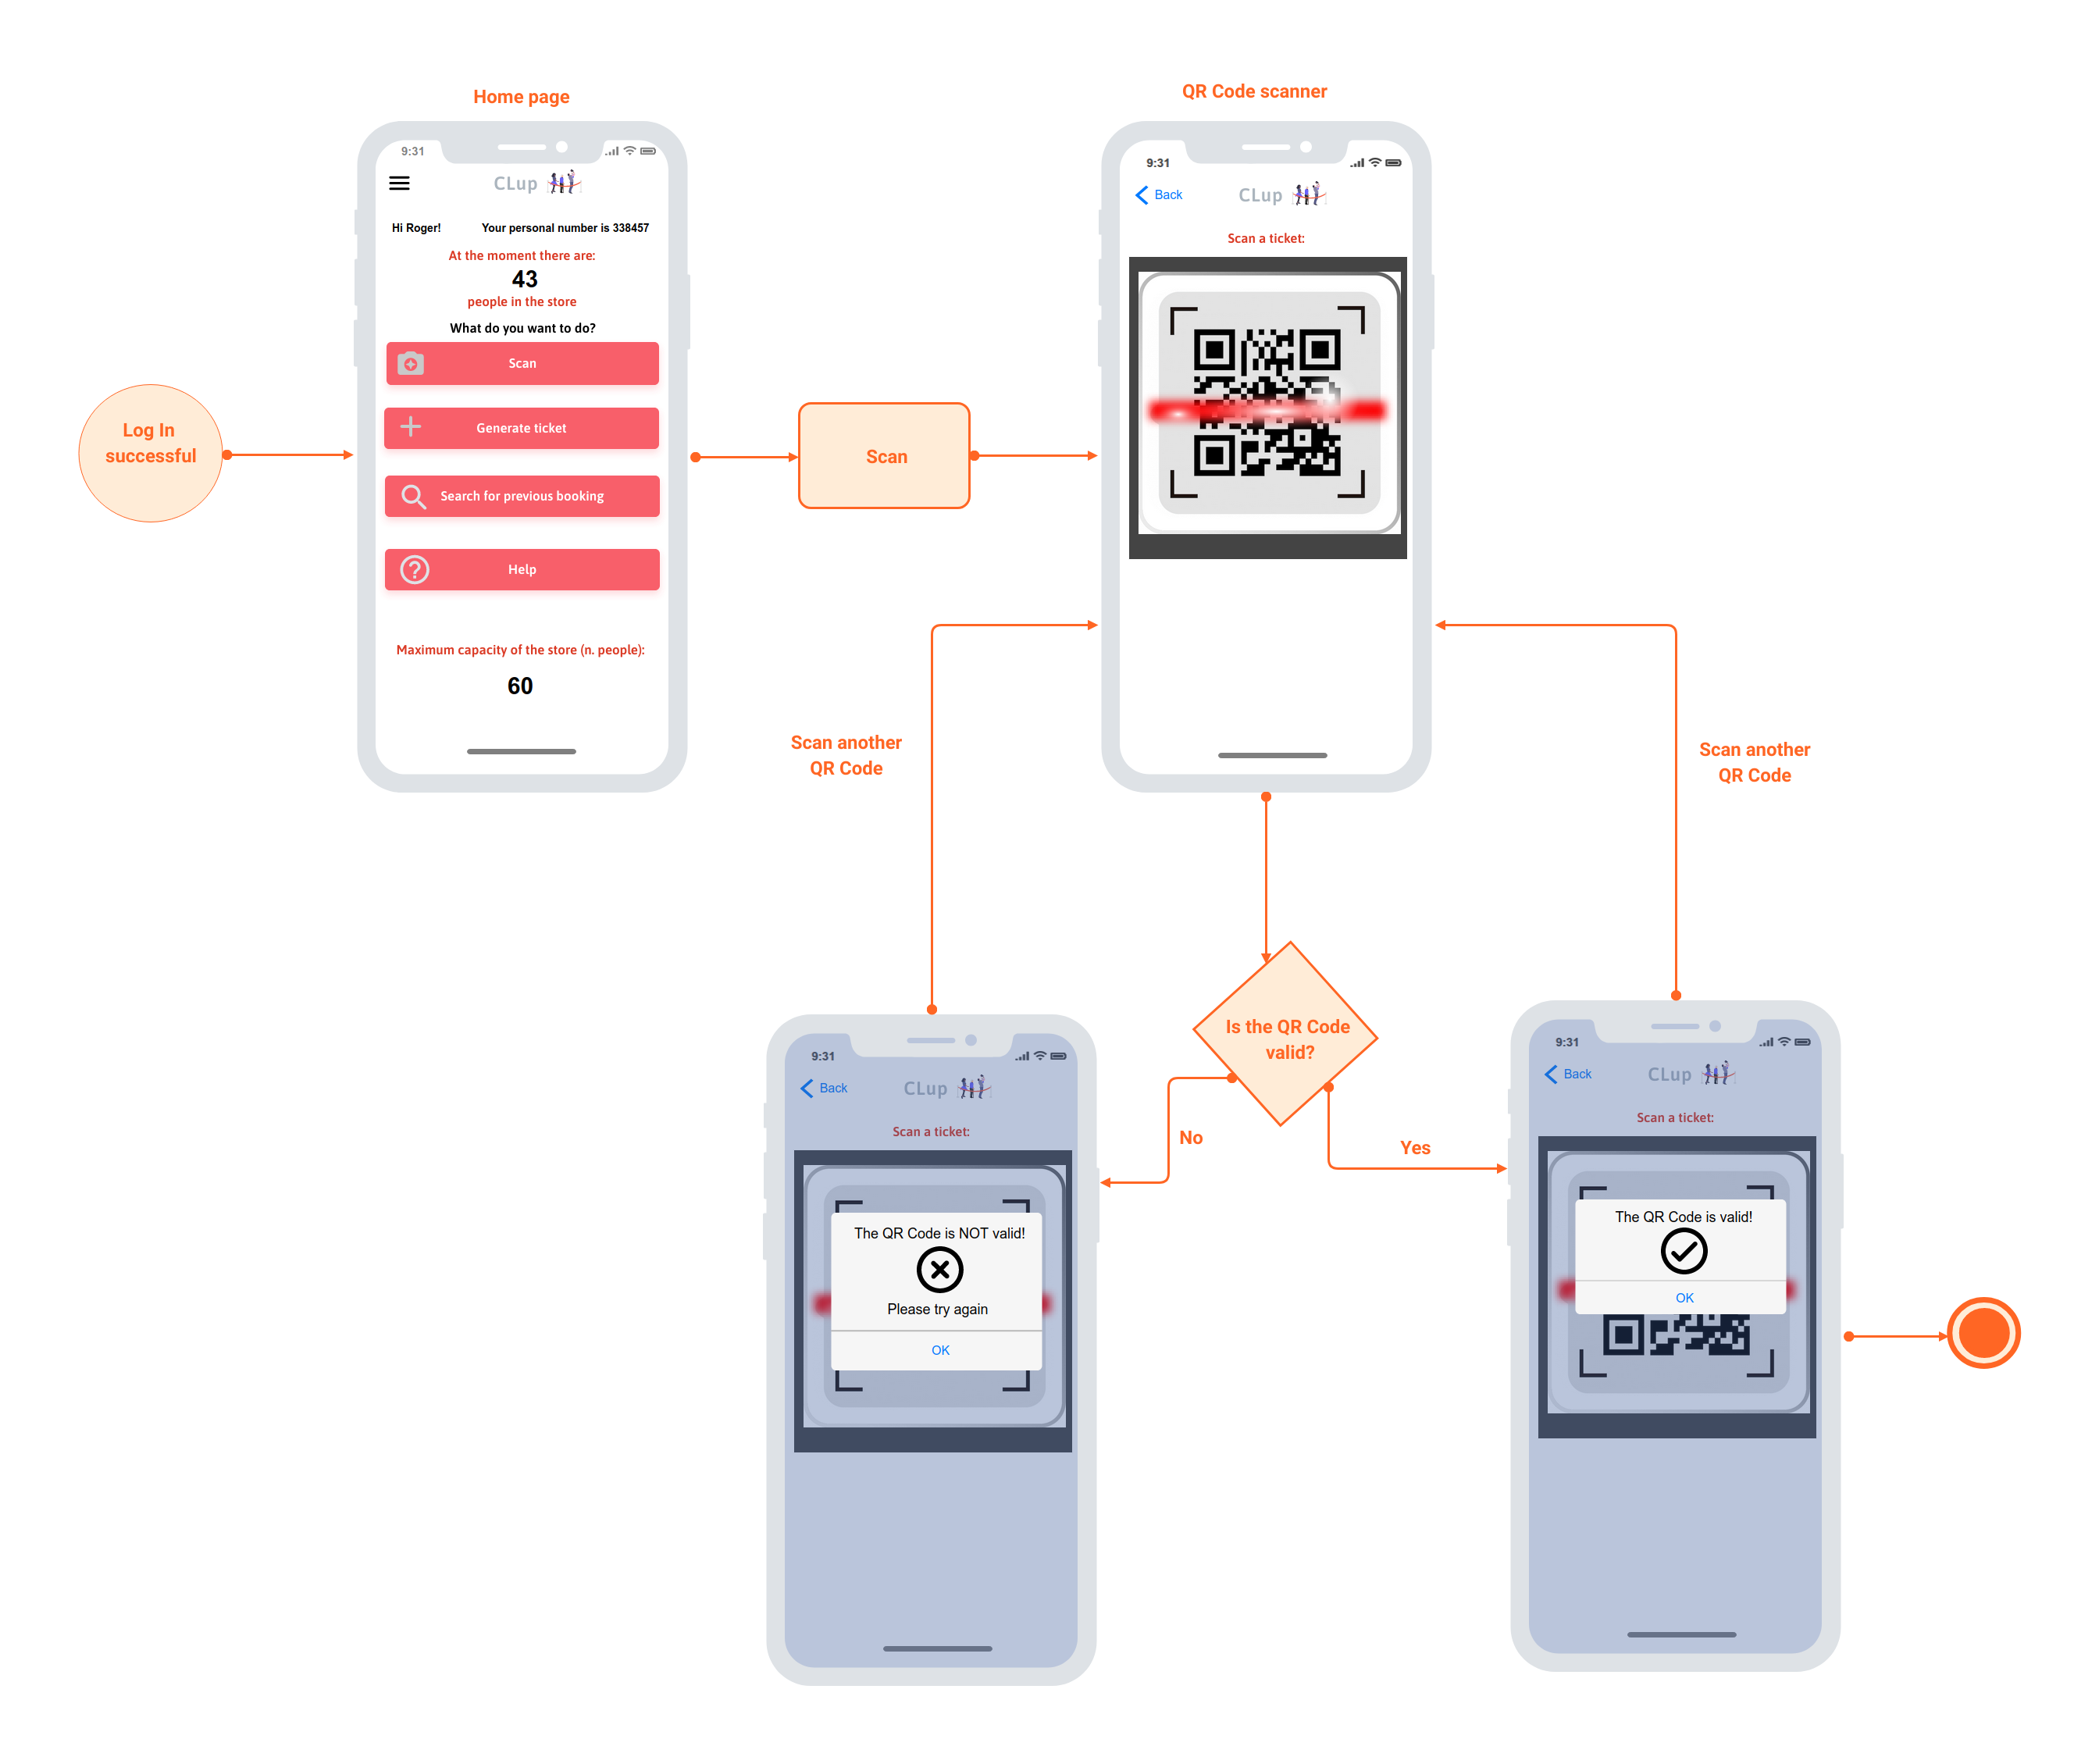
\includegraphics[width=\textwidth]{assets/User-Interface-Design/scan_qr_attendant.png}
        \caption{Scan QR Code}
    \end{figure}
\end{center}

\begin{center}
    \begin{figure}[H]
        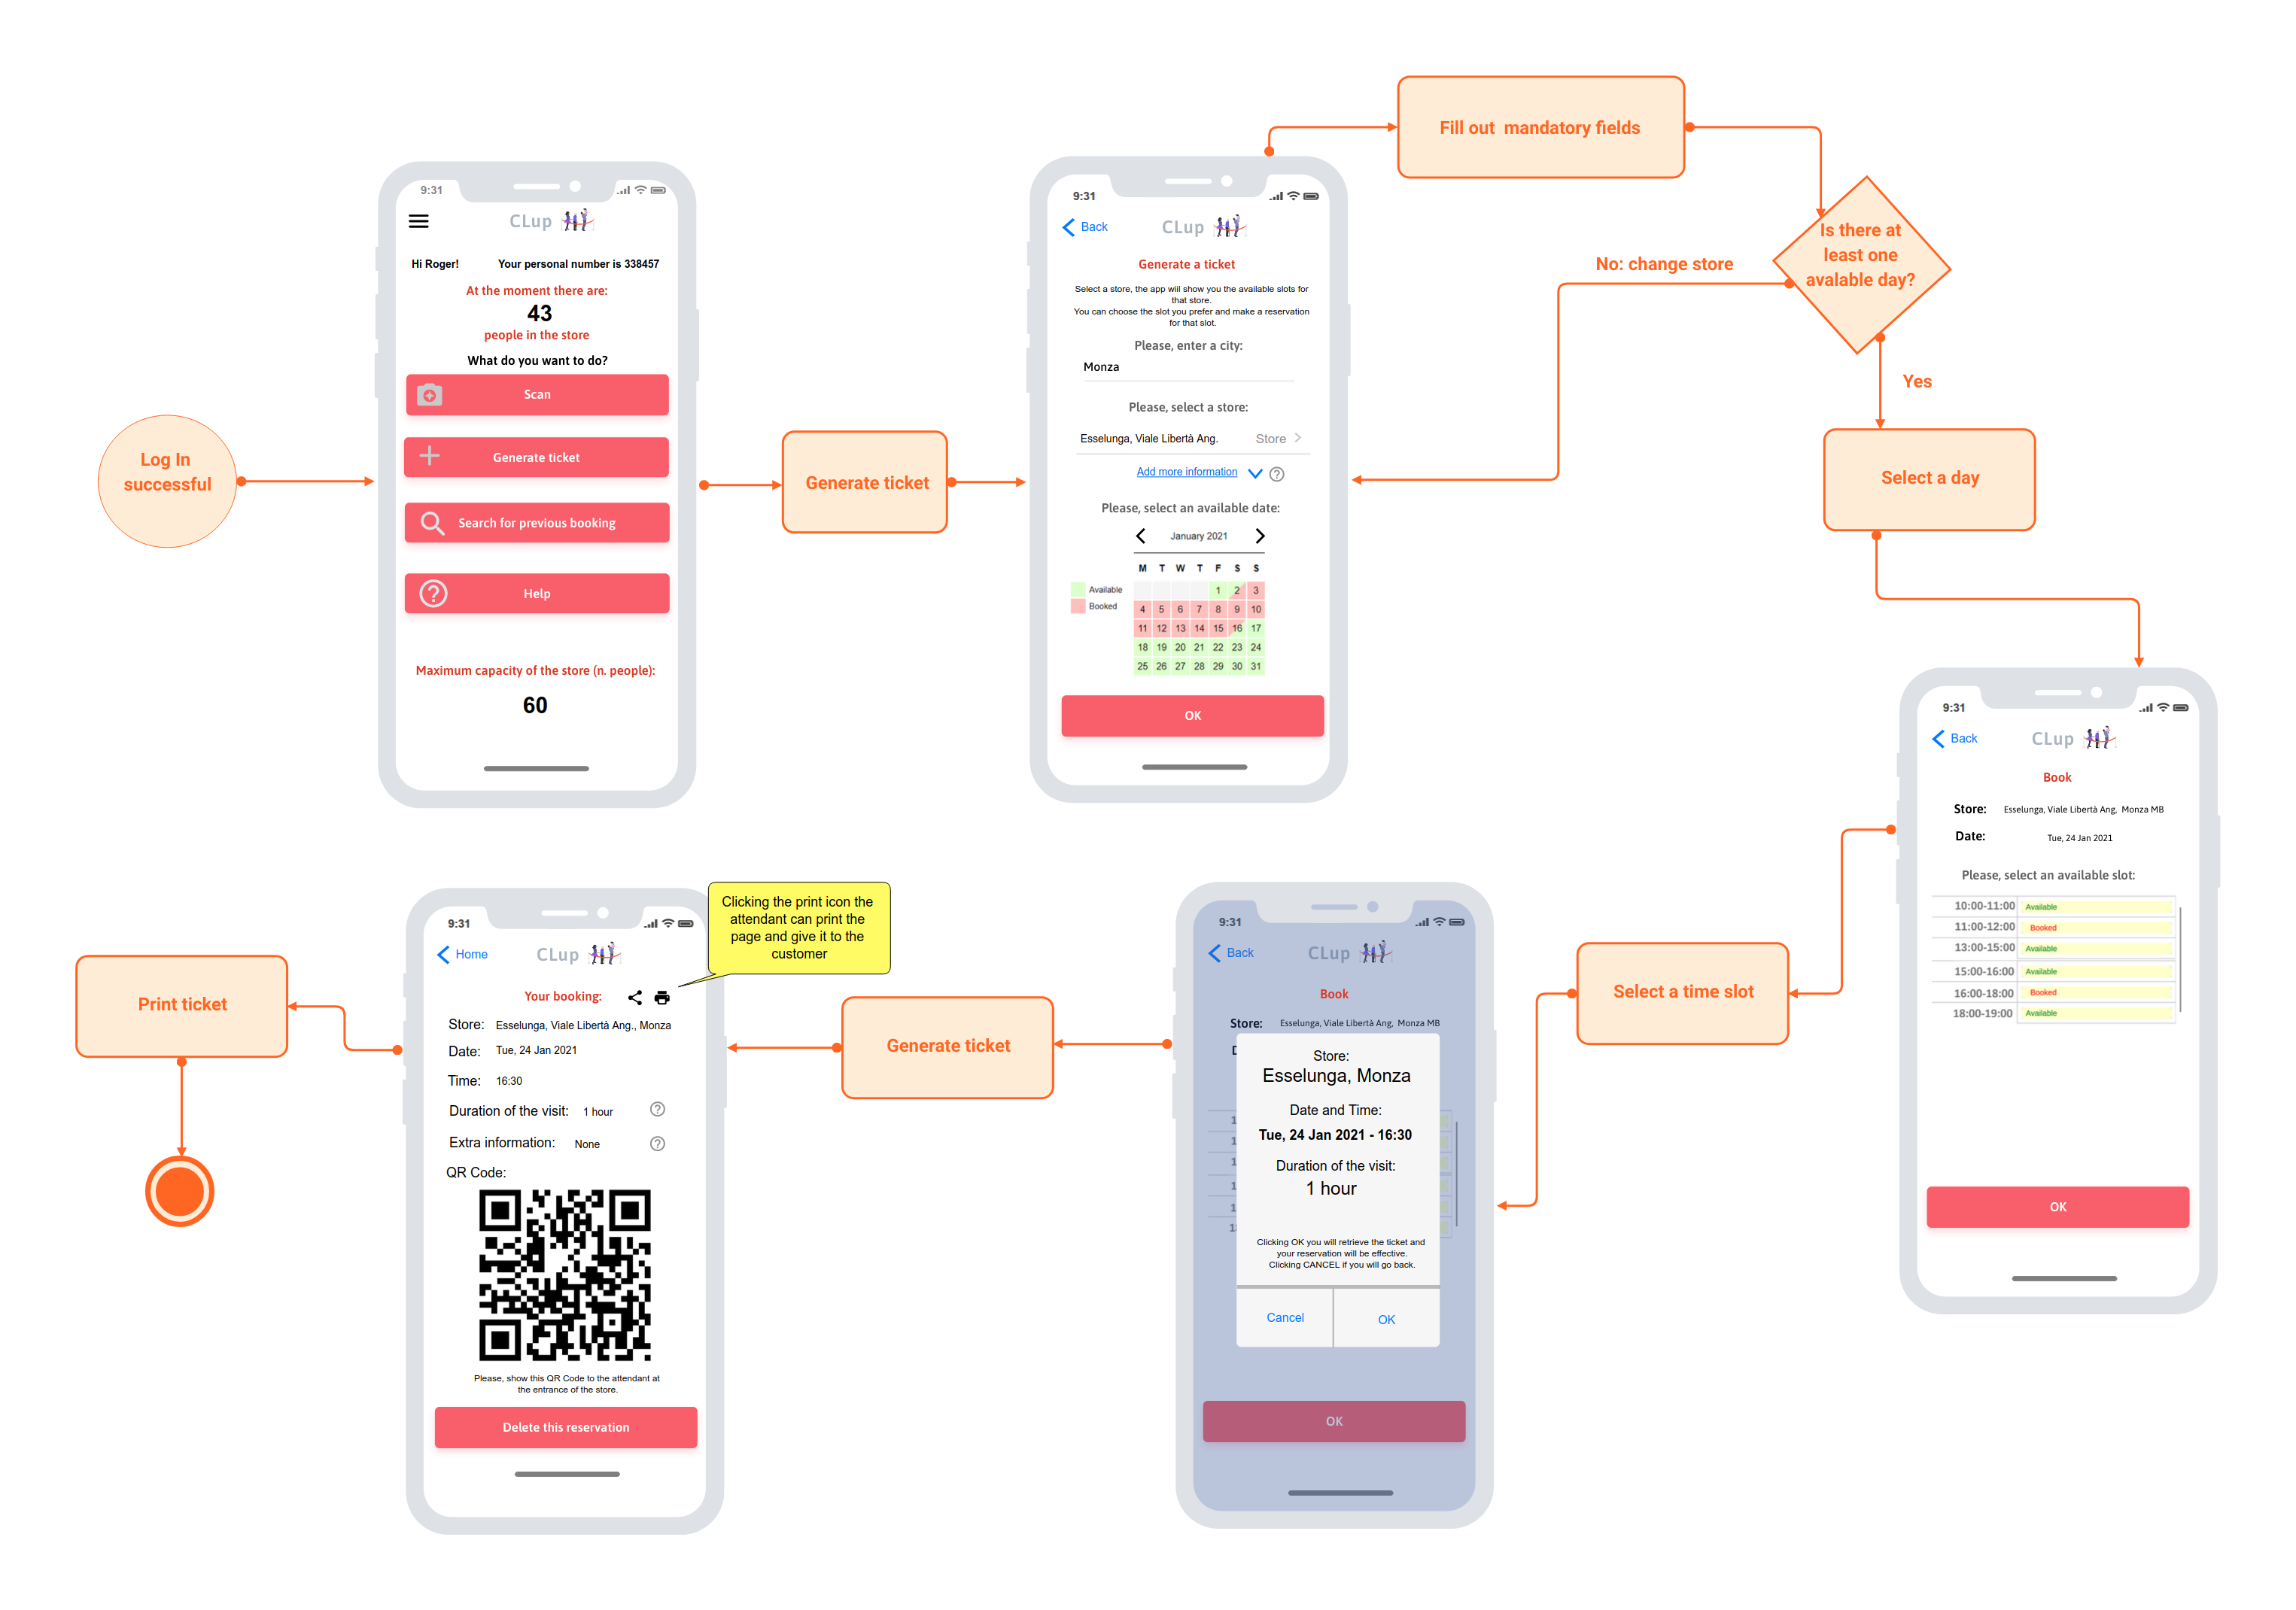
\includegraphics[width=\textwidth]{assets/User-Interface-Design/generate_ticket_attendant.png}
        \caption{Release ticket on spot}
    \end{figure}
\end{center}

\subsection{Store Administrator Web Interface}
\begin{center}
    \begin{figure}[H]
        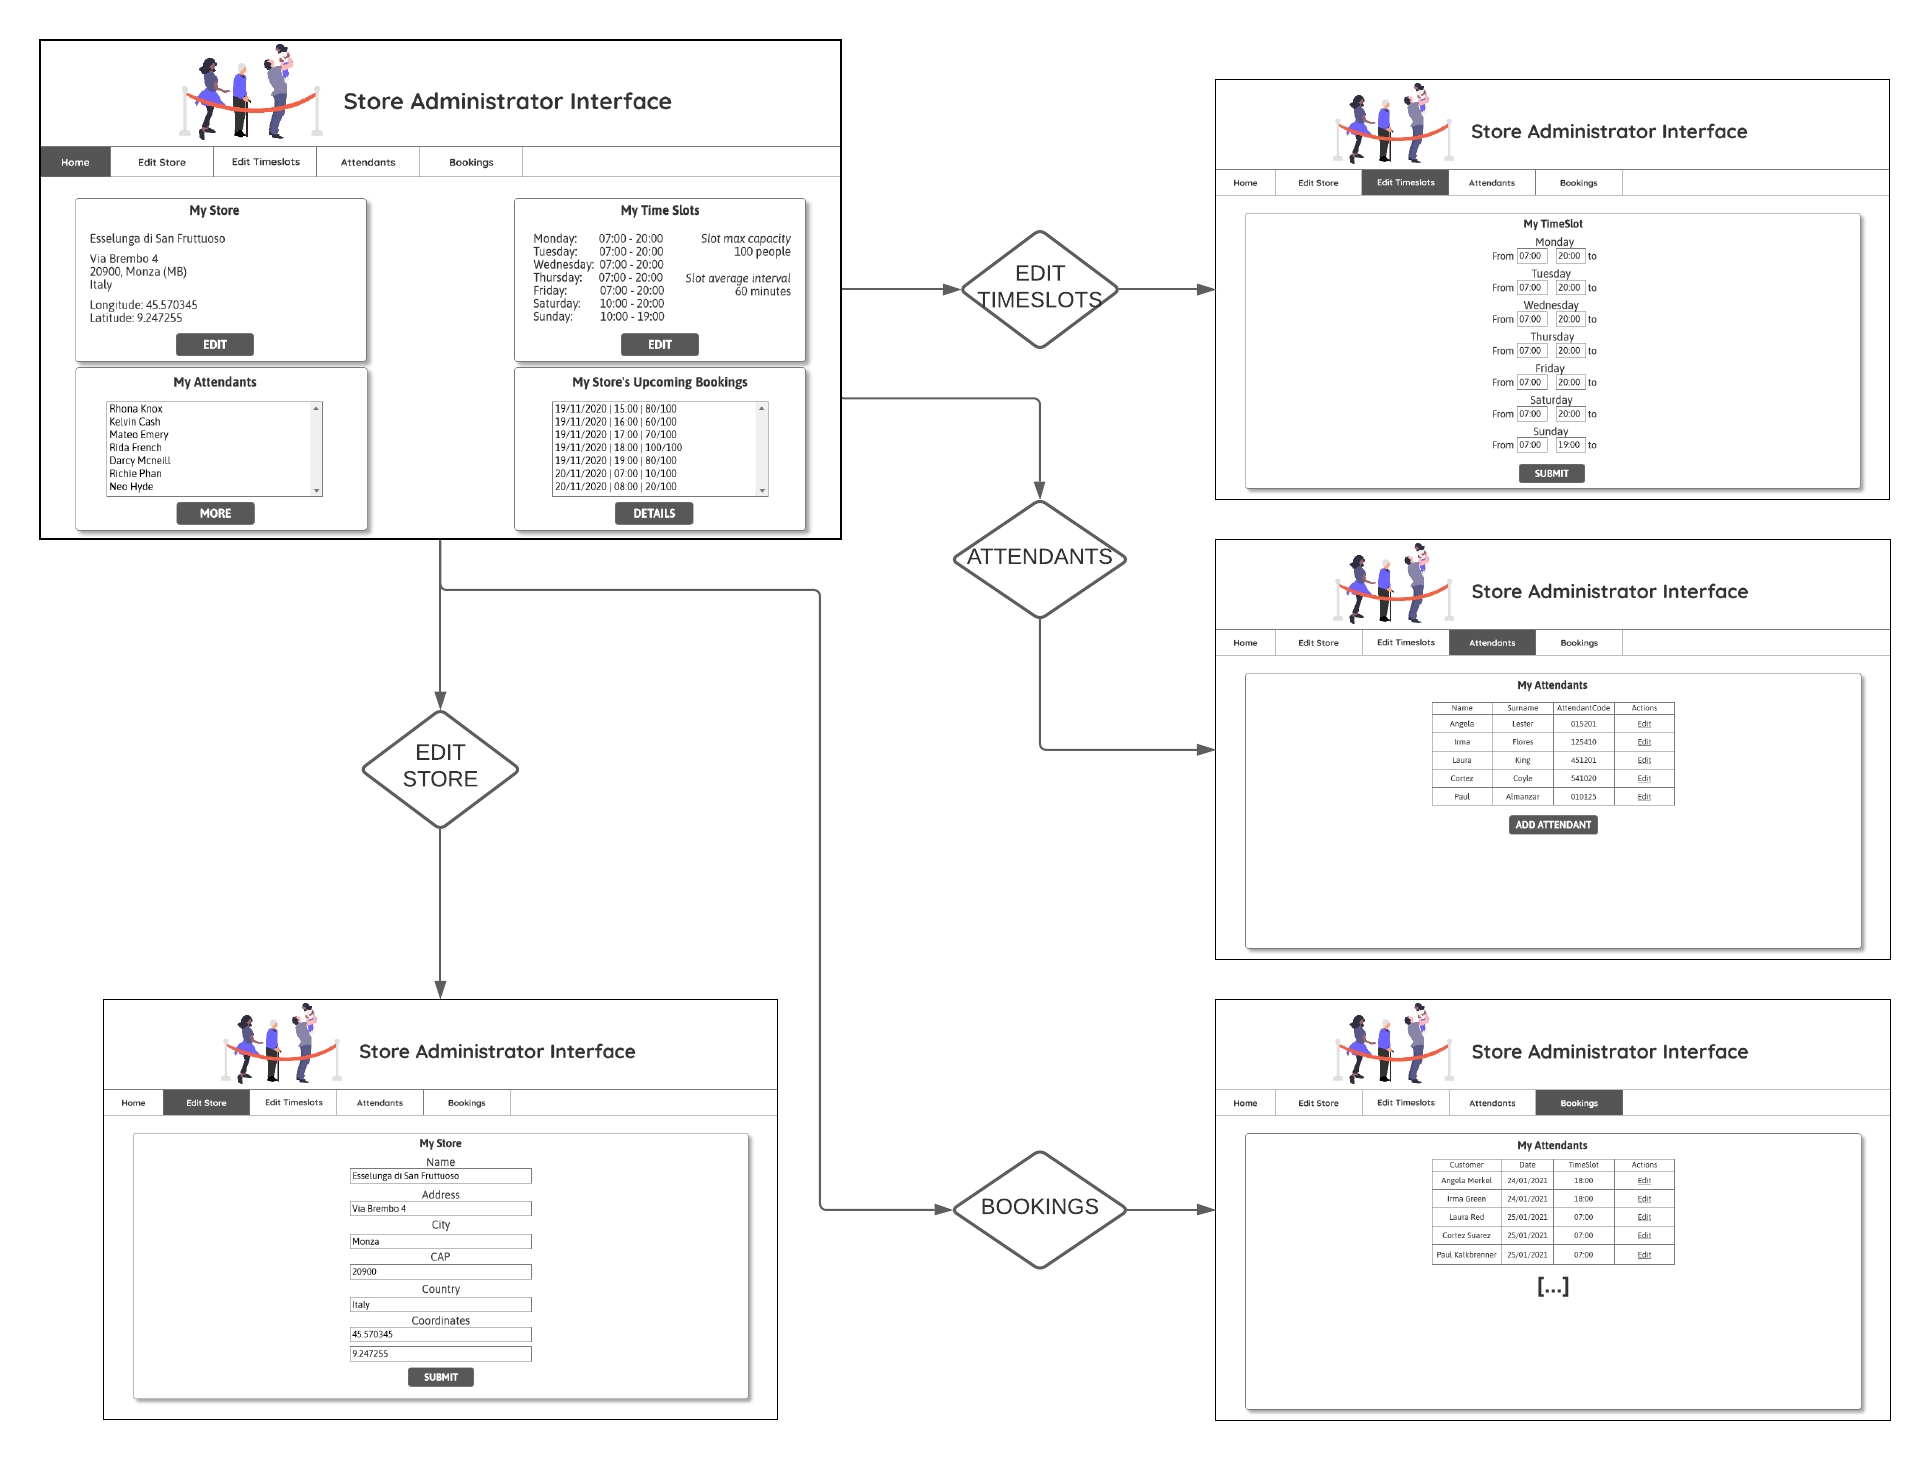
\includegraphics[width=\textwidth]{assets/Mockups/MockUpStoreAdmin.png}
        \caption{Store Administrator Interface}
    \end{figure}
\end{center}

\section{Requirements Traceability}
This section will shown the traceability between requirements and modules described in component diagram.

\begin{itemize}
    \item \textbf{R1:} The system allows registered users to select the store where they want to shop
          \begin{itemize}
              \item \textbf{Login Handler}: this module allows registered users to select a store if they provide a correct combination of username and password.
              \item \textbf{ASAP Handler} \textit{or} \textbf{Reservation Handler:} this module allows to select a store either in case of ASAP functionality choice or Reservation functionality choice.
          \end{itemize}
    \item \textbf{R2:} The system allows users to retrieve a queue number
          \begin{itemize}
              \item \textbf{ASAP Handler}
              \item \textbf{Generate on spot:} this module allows people who are not registered to CLup service to be queued up manually by the store attendants.
          \end{itemize}
    \item \textbf{R3:} The system generates a QR Code associated to the ticket
          \begin{itemize}
              \item \textbf{QRCode Generator:} this component allows the QRCode to be generated from the ticket id.
          \end{itemize}
    \item \textbf{R4:} The system allows Store Administrators to add GPS Position and opening hours of the store
          \begin{itemize}
              \item \textbf{Store Management:} this module allows store administrator to edit all the information about their stores.
          \end{itemize}
    \item \textbf{R5:} The system allows Store Attendants to register with their attendant code
          \begin{itemize}
              \item \textbf{Sign Up:} this module allows the three types of users to register to the platform of CLup.
          \end{itemize}
    \item \textbf{R6:} The system allows users to select a day/time slot from the available ones
          \begin{itemize}
              \item \textbf{Reservation Handler:} this module allows to accomplish to book a visit functionality.
          \end{itemize}
    \item \textbf{R7:} The system allows users to add a list of products (categories) to purchase and the duration time of the visit
          \begin{itemize}
              \item \textbf{Reservation Handler}
          \end{itemize}
    \item \textbf{R8:} The system computes a prediction of expected time duration of a customer's visit
          \begin{itemize}
              \item \textbf{AlternativeSlotRecommender} this component lets the system suggests alternative choices relying on people past bookings.
          \end{itemize}
    \item \textbf{R9:} The system recommends alternative day/time slots or store/chains to a user
          \begin{itemize}
              \item \textbf{Alternative slot recommender}
          \end{itemize}
    \item \textbf{R10:} The system takes note about the actual queue number
          \begin{itemize}
              \item \textbf{ASAP Handler} \textit{or} \textbf{Reservation Handler}
          \end{itemize}
    \item \textbf{R11:} The system notifies the user when its queue number is going to be called
          \begin{itemize}
              \item \textbf{Notification Handler:} this module triggers an action when a number is going to be called and informs the user through a notification.
          \end{itemize}
\end{itemize}

Also the system attributes are guaranteed by the design choices explained in this document; more precisely:
\begin{itemize}
    \item \textbf{Easy usability}: guaranteed through a very simple, minimal and intuitive user interface. Since the main target of the application is the customer-side, the experience is designed to be very simple. In fact, there are only a few buttons with clear and precise functionalities. The aim is to complete the \textit{ASAP} ticket retrieval in no more than five taps (or clicks).
    \item \textbf{Reliability and Availability}: accomplished through a replication of the running application in different clones, following the \textit{scale-out} method. The physical nodes of the system would then work in parallel, avoiding system downtimes due to a failure. In fact, when a clone breaks down, there are others in parallel which can supply the requested service, but with some performance issues. The scope is to obtain at least 97\% of availability for each tier (the total system would then have 97\% of availability).
    \item \textbf{Security}: guaranteed through an encrypted communication between client and server. If the client is connecting through the web interface, connection moves on HTTPS protocol. Otherwise, connection goes on TLS protocol.
    \item \textbf{Cross Platform}: firstly obtained through a development of a web interface, which can be accessed from any type of connected device with a browser installed. The native mobile application, instead, will be available only for iOS and Android users and will be downloadable from App Store and Google Play.
    \item \textbf{Maintainability and Modularity:} the first is accomplished through the second, because the application will be divided in some small parts (called modules) which interacts each other to provide the requested service.
\end{itemize}

\section{Implementation, Integration and Test Plan}
The S2B will be divided as follows:
\begin{itemize}
    \item Client: it includes either web browser or mobile application;
    \item Web Server;
    \item Application Server;
    \item Internal Database;
    \item External services (such as OpenStreetMaps, IdP providers, etc).
\end{itemize}

These elements will be implemented following a bottom up logic, in order to avoid stub structures that would be more difficult to implement and test.

The main focus is on the module of the application server, because of its importance in the S2B development and also due to its testing difficulty.

The following table presents the functionalities described in the RASD document and highlight for each of them the importance for the customer and the difficulty of their implementation.

\begin{center}
    \begin{table}[H]
        \begin{tabular}{ | c |c | c | c |}
            \hline
            \textbf{Functionality} & \textbf{Module} & \textbf{Importance for customer} & \textbf{Difficulty} \\ \hline
            Sign Up and Login      & 1 (MVP)         & Low                              & Low                 \\ \hline
            ASAP                   & 1 (MVP)         & High                             & Medium              \\\hline
            Make a reservation     & 2               & Medium                           & High                \\\hline
            Hand out on spot       & 1 (MVP)         & High                             & Medium              \\\hline
            Periodic notifications & 1 (MVP)         & Low                              & High                \\
            \hline
        \end{tabular}
        \caption{Implementation and Testing precedences}\label{implementation_precedences}
    \end{table}
\end{center}

All the modules described in this document rely on DBMS of the internal database, which must be implemented as the first component.

According to the table\ref{implementation_precedences} we decided to implement the functionalities relying on their importance.

\begin{itemize}
    \item \textbf{ASAP:} for this functionality it is necessary to implement and execute tests on the ASAPHandler and the QRCode Generation component. The ASAP handler is tested through an appropriate choice of store and through a check about the assigned time slot. The QRCode Generation is tested through a check on the content of it, which can also test the functionality of the QRCode Validation component.
    \item \textbf{Hand out on spot:} this functionality is managed by the GenerateOnSpot component, on which the unit tests will be made. They will check that the module manages in a correct way all the requests of ticket that are made on spot, by an attendant of the considered store. Finally, an integration test with the DBMS is made.
    \item \textbf{Make a reservation:} this module is an extension of the MVP one. It exploits some components, which are the ReservationHandler, AlternativeSlotRecommender, QRCode Validation and QRCode Generation ones. They will need some unit tests and, in particular, the ReservationHandler one also needs an integration test with the DBMS.
    \item \textbf{SignUp and Login:} the two functionalities are strictly related, since the Login result is somehow affected by the SignUp function. So it would be a good idea to implement the SignUpHandler first and then the LoginHandler and then execute a unit and integration test. The test of the SignUpHandler requires a demo of the DBMS containing some accounts. In fact it’s necessary to test the correct call to the DBMS functions in order to retrieve the account already registered and then it is important to check the module recognize when a user is already registered or if the sent data presents some inconsistencies. Relying on the DBMS functions, an integration test is required to check the correct communication between the module and DBMS. These tests must also be executed for the LoginHandler because it retrieves data from the database to execute credentials check.
    \item \textbf{Periodic notifications:} this functionality is accomplished through the NotificationHandler, on which some unit tests are needed to be executed. To properly make this tests, a demo scenario is needed, in which a customer retrieves a ticket (through, for example, the ASAP functionality) and the system triggers because the ticket is going to be called.
\end{itemize}

\subsection{Clarification on component integration}
In this section there is be a description about how the components are integrated and communicate, in order to build the entire S2B.

First of all, in figure\ref{components_integration} it is clear that the first component to build is the DBMS, followed by the main application components that exploit it.

\begin{center}
    \begin{figure}[H]
        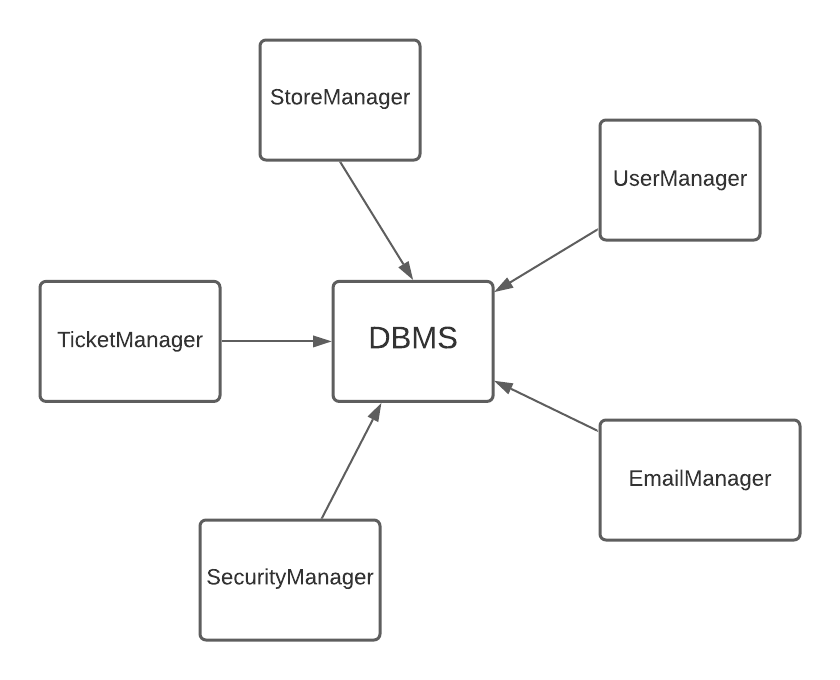
\includegraphics[width=\textwidth]{assets/IT-Plan/Components-Integration.png}
        \caption{Components Integration}\label{components_integration}
    \end{figure}
\end{center}


After this, we have to integrate the API communication between the S2B and the external services that will be used, which are some \textit{IdP} providers, as explained in figure\ref{external_services}.

\begin{center}
    \begin{figure}[H]
        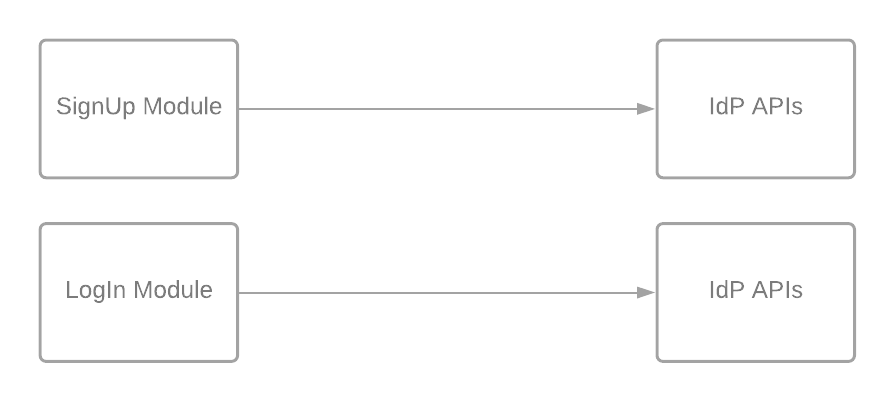
\includegraphics[width=\textwidth]{assets/IT-Plan/External-Services.png}
        \caption{External APIs integrations}\label{external_services}
    \end{figure}
\end{center}

At this point it is possible to integrate the Client Manager, which permits to the end user to exploit all the functionalities, as shown in figure\ref{client_manager}.

\begin{center}
    \begin{figure}[H]
        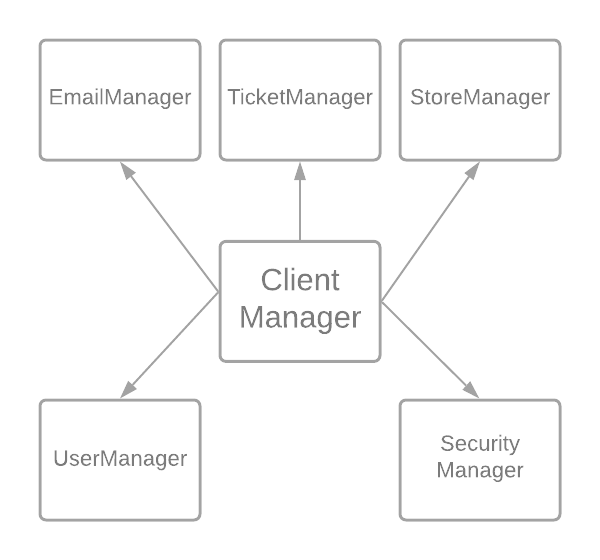
\includegraphics[width=\textwidth]{assets/IT-Plan/ClientManager.png}
        \caption{Client Manager Integration}\label{client_manager}
    \end{figure}
\end{center}

Finally, it is possible to integrate the web server module and the mobile application module and the browser with the web server module. This work in necessary in order to make possible the client-server communication.

This last part is shown in figure\ref{client_server_integration}.

Together with this, as shown in figure\ref{maps_api}, the client will be integrated with the maps API, which are provided by \textit{OpenStreetMaps}.

\begin{center}
    \begin{figure}[H]
        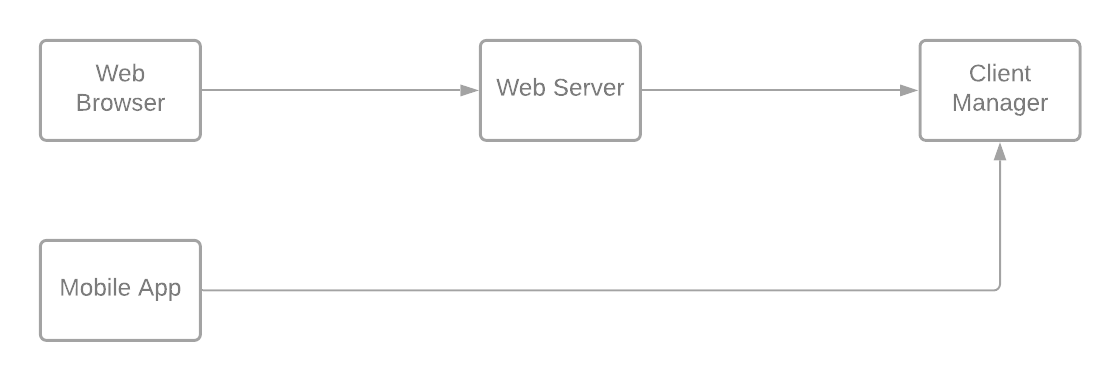
\includegraphics[width=\textwidth]{assets/IT-Plan/ClientServerIntegration.png}
        \caption{Client-Server Integration}\label{client_server_integration}
    \end{figure}
\end{center}

\begin{center}
    \begin{figure}[H]
        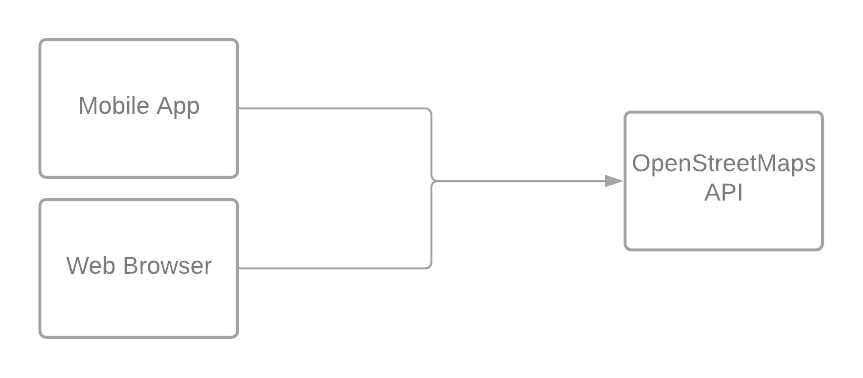
\includegraphics[width=\textwidth]{assets/IT-Plan/OpenStreetMaps.png}
        \caption{Client-Side Maps Integration}\label{maps_api}
    \end{figure}
\end{center}


\pagestyle{plain}

\section{Effort spent}
\begin{tabular}{ | c || c | c | c | c| c|}
    \hline
    Student        & Time for S.1 & S.2 & Time for S.3 & Time for S.4 & Time for S.5 \\ \hline
    Alice Piemonti & 2h           & 3h  & 6h           & 1h           & 1h           \\ \hline
    Luca Pirovano  & 2h           & 7h  & 2h           & 2h           & 2h           \\ \hline
    Nicolò Sonnino & 3h           & 7h  & 2h           & 2h           & 2h           \\
    \hline
\end{tabular}

\end{document}
